\documentclass[a4paper]{book}
\usepackage{makeidx}
\usepackage{graphicx}
\usepackage{multicol}
\usepackage{float}
\usepackage{listings}
\usepackage{color}
\usepackage{ifthen}
\usepackage[table]{xcolor}
\usepackage{textcomp}
\usepackage{alltt}
\usepackage{ifpdf}
\ifpdf
\usepackage[pdftex,
            pagebackref=true,
            colorlinks=true,
            linkcolor=blue,
            unicode
           ]{hyperref}
\else
\usepackage[ps2pdf,
            pagebackref=true,
            colorlinks=true,
            linkcolor=blue,
            unicode
           ]{hyperref}
\usepackage{pspicture}
\fi
\usepackage[utf8]{inputenc}
\usepackage{mathptmx}
\usepackage[scaled=.90]{helvet}
\usepackage{courier}
\usepackage{doxygen}
\lstset{language=C++,inputencoding=utf8,basicstyle=\footnotesize,breaklines=true,breakatwhitespace=true,tabsize=8,numbers=left }
\makeindex
\setcounter{tocdepth}{3}
\renewcommand{\footrulewidth}{0.4pt}
\begin{document}
\hypersetup{pageanchor=false}
\begin{titlepage}
\vspace*{7cm}
\begin{center}
{\Large Reference Manual}\\
\vspace*{1cm}
{\large Generated by Doxygen 1.7.3}\\
\vspace*{0.5cm}
{\small Mon Dec 5 2011 00:02:23}\\
\end{center}
\end{titlepage}
\clearemptydoublepage
\pagenumbering{roman}
\tableofcontents
\clearemptydoublepage
\pagenumbering{arabic}
\hypersetup{pageanchor=true}
\chapter{Class Index}
\section{Class Hierarchy}
This inheritance list is sorted roughly, but not completely, alphabetically:\begin{DoxyCompactList}
\item \contentsline{section}{Action}{\pageref{classAction}}{}
\item \contentsline{section}{Brain}{\pageref{classBrain}}{}
\item \contentsline{section}{Field}{\pageref{classField}}{}
\item \contentsline{section}{FullBackBrain}{\pageref{classFullBackBrain}}{}
\item \contentsline{section}{Game}{\pageref{classGame}}{}
\item \contentsline{section}{GoalieBrain}{\pageref{classGoalieBrain}}{}
\item \contentsline{section}{MathHelp}{\pageref{classMathHelp}}{}
\item \contentsline{section}{Memory}{\pageref{classMemory}}{}
\item \contentsline{section}{Mode}{\pageref{classMode}}{}
\item \contentsline{section}{ObjInfo}{\pageref{classObjInfo}}{}
\begin{DoxyCompactList}
\item \contentsline{section}{ObjBall}{\pageref{classObjBall}}{}
\item \contentsline{section}{ObjFlag}{\pageref{classObjFlag}}{}
\item \contentsline{section}{ObjGoal}{\pageref{classObjGoal}}{}
\item \contentsline{section}{ObjLine}{\pageref{classObjLine}}{}
\item \contentsline{section}{ObjPlayer}{\pageref{classObjPlayer}}{}
\end{DoxyCompactList}
\item \contentsline{section}{ObjMemory}{\pageref{classObjMemory}}{}
\item \contentsline{section}{Parser}{\pageref{classParser}}{}
\item \contentsline{section}{Player}{\pageref{classPlayer}}{}
\begin{DoxyCompactList}
\item \contentsline{section}{Forward}{\pageref{classForward}}{}
\item \contentsline{section}{FullBack}{\pageref{classFullBack}}{}
\item \contentsline{section}{Goalie}{\pageref{classGoalie}}{}
\end{DoxyCompactList}
\item \contentsline{section}{Polar}{\pageref{classPolar}}{}
\item \contentsline{section}{Pos}{\pageref{classPos}}{}
\item \contentsline{section}{RoboClient}{\pageref{classRoboClient}}{}
\item \contentsline{section}{SenseMemory}{\pageref{classSenseMemory}}{}
\end{DoxyCompactList}

\chapter{Class Index}
\section{Class List}
Here are the classes, structs, unions and interfaces with brief descriptions:\begin{DoxyCompactList}
\item\contentsline{section}{\hyperlink{classAction}{Action} }{\pageref{classAction}}{}
\item\contentsline{section}{\hyperlink{classBrain}{Brain} }{\pageref{classBrain}}{}
\item\contentsline{section}{\hyperlink{classField}{Field} }{\pageref{classField}}{}
\item\contentsline{section}{\hyperlink{classForward}{Forward} }{\pageref{classForward}}{}
\item\contentsline{section}{\hyperlink{classFullBack}{FullBack} }{\pageref{classFullBack}}{}
\item\contentsline{section}{\hyperlink{classFullBackBrain}{FullBackBrain} }{\pageref{classFullBackBrain}}{}
\item\contentsline{section}{\hyperlink{classGame}{Game} }{\pageref{classGame}}{}
\item\contentsline{section}{\hyperlink{classGoalie}{Goalie} }{\pageref{classGoalie}}{}
\item\contentsline{section}{\hyperlink{classGoalieBrain}{GoalieBrain} }{\pageref{classGoalieBrain}}{}
\item\contentsline{section}{\hyperlink{classMathHelp}{MathHelp} }{\pageref{classMathHelp}}{}
\item\contentsline{section}{\hyperlink{classMemory}{Memory} }{\pageref{classMemory}}{}
\item\contentsline{section}{\hyperlink{classMode}{Mode} }{\pageref{classMode}}{}
\item\contentsline{section}{\hyperlink{classObjBall}{ObjBall} }{\pageref{classObjBall}}{}
\item\contentsline{section}{\hyperlink{classObjFlag}{ObjFlag} }{\pageref{classObjFlag}}{}
\item\contentsline{section}{\hyperlink{classObjGoal}{ObjGoal} }{\pageref{classObjGoal}}{}
\item\contentsline{section}{\hyperlink{classObjInfo}{ObjInfo} }{\pageref{classObjInfo}}{}
\item\contentsline{section}{\hyperlink{classObjLine}{ObjLine} }{\pageref{classObjLine}}{}
\item\contentsline{section}{\hyperlink{classObjMemory}{ObjMemory} }{\pageref{classObjMemory}}{}
\item\contentsline{section}{\hyperlink{classObjPlayer}{ObjPlayer} }{\pageref{classObjPlayer}}{}
\item\contentsline{section}{\hyperlink{classParser}{Parser} }{\pageref{classParser}}{}
\item\contentsline{section}{\hyperlink{classPlayer}{Player} }{\pageref{classPlayer}}{}
\item\contentsline{section}{\hyperlink{classPolar}{Polar} }{\pageref{classPolar}}{}
\item\contentsline{section}{\hyperlink{classPos}{Pos} }{\pageref{classPos}}{}
\item\contentsline{section}{\hyperlink{classRoboClient}{RoboClient} }{\pageref{classRoboClient}}{}
\item\contentsline{section}{\hyperlink{classSenseMemory}{SenseMemory} }{\pageref{classSenseMemory}}{}
\end{DoxyCompactList}

\chapter{File Index}
\section{File List}
Here is a list of all documented files with brief descriptions:\begin{DoxyCompactList}
\item\contentsline{section}{\hyperlink{Action_8java}{Action.java} }{\pageref{Action_8java}}{}
\item\contentsline{section}{\hyperlink{Brain_8java}{Brain.java} }{\pageref{Brain_8java}}{}
\item\contentsline{section}{\hyperlink{Field_8java}{Field.java} }{\pageref{Field_8java}}{}
\item\contentsline{section}{\hyperlink{Forward_8java}{Forward.java} }{\pageref{Forward_8java}}{}
\item\contentsline{section}{\hyperlink{FullBack_8java}{FullBack.java} }{\pageref{FullBack_8java}}{}
\item\contentsline{section}{\hyperlink{Game_8java}{Game.java} }{\pageref{Game_8java}}{}
\item\contentsline{section}{\hyperlink{Goalie_8java}{Goalie.java} }{\pageref{Goalie_8java}}{}
\item\contentsline{section}{\hyperlink{MathHelp_8java}{MathHelp.java} }{\pageref{MathHelp_8java}}{}
\item\contentsline{section}{\hyperlink{Memory_8java}{Memory.java} }{\pageref{Memory_8java}}{}
\item\contentsline{section}{\hyperlink{Mode_8java}{Mode.java} }{\pageref{Mode_8java}}{}
\item\contentsline{section}{\hyperlink{ObjInfo_8java}{ObjInfo.java} }{\pageref{ObjInfo_8java}}{}
\item\contentsline{section}{\hyperlink{ObjMemory_8java}{ObjMemory.java} }{\pageref{ObjMemory_8java}}{}
\item\contentsline{section}{\hyperlink{Parser_8java}{Parser.java} }{\pageref{Parser_8java}}{}
\item\contentsline{section}{\hyperlink{Player_8java}{Player.java} }{\pageref{Player_8java}}{}
\item\contentsline{section}{\hyperlink{Pos_8java}{Pos.java} }{\pageref{Pos_8java}}{}
\item\contentsline{section}{\hyperlink{RoboClient_8java}{RoboClient.java} }{\pageref{RoboClient_8java}}{}
\item\contentsline{section}{\hyperlink{SenseMemory_8java}{SenseMemory.java} }{\pageref{SenseMemory_8java}}{}
\end{DoxyCompactList}

\chapter{Class Documentation}
\hypertarget{classAction}{
\section{Action Class Reference}
\label{classAction}\index{Action@{Action}}
}
\subsection*{Public Member Functions}
\begin{DoxyCompactItemize}
\item 
\hyperlink{classAction_a4f457ccfc8336b565cadca56b36e0271}{Action} ()
\item 
\hyperlink{classAction_acfa1602ef29e16a6047cc058ff0a16ac}{Action} (\hyperlink{classMemory}{Memory} mem, \hyperlink{classRoboClient}{RoboClient} rc)
\item 
void \hyperlink{classAction_a4f775977b788d1379b9f6c45bb37c01f}{setMem} (\hyperlink{classMemory}{Memory} mem)
\item 
double \hyperlink{classAction_ad68c5200162e4023fb88488e340ea454}{getTurn} (\hyperlink{classPolar}{Polar} go)
\item 
void \hyperlink{classAction_a6b7099c20c56fc3dd72ce4c8ba4f3870}{gotoPoint} (\hyperlink{classPolar}{Polar} go)
\item 
void \hyperlink{classAction_a653bde47fe3bd4263ed31095e2ee1cfc}{gotoSidePoint} (\hyperlink{classPos}{Pos} p)
\item 
void \hyperlink{classAction_a5f7eb7be5b6b18854936367833044a6e}{gotoPoint} (\hyperlink{classPos}{Pos} p)
\item 
void \hyperlink{classAction_abf9085a62947a12cc2e154396177ec90}{goHome} ()
\item 
void \hyperlink{classAction_a49e1c7f1d7f5a4294c93833997603339}{findBall} ()  throws UnknownHostException, InterruptedException 
\item 
\hypertarget{classAction_a79224f655b7f92fe9a334bf96a01e844}{
void {\bfseries kickOff} ()  throws UnknownHostException, InterruptedException }
\label{classAction_a79224f655b7f92fe9a334bf96a01e844}

\item 
\hyperlink{classObjPlayer}{ObjPlayer} \hyperlink{classAction_a63d035f7132842d9720b88247d525112}{closestPlayer} ()  throws UnknownHostException, InterruptedException 
\item 
void \hyperlink{classAction_a55e146013466e96013a196d9bd787410}{passBall} (\hyperlink{classObjBall}{ObjBall} ball, \hyperlink{classObjPlayer}{ObjPlayer} p)
\item 
void \hyperlink{classAction_a9e883bc90ec59c4eeb5b0b3dd022b33a}{FullBack\_\-findBall} ()  throws UnknownHostException, InterruptedException 
\item 
void \hyperlink{classAction_ad7308d47f6303c20834dda533d4fe793}{kickToPoint} (\hyperlink{classObjBall}{ObjBall} ball, \hyperlink{classPolar}{Polar} p)
\item 
void \hyperlink{classAction_a639b23a22badac8eb8603bc153daba99}{kickToPoint} (\hyperlink{classObjBall}{ObjBall} ball, \hyperlink{classPos}{Pos} p)
\item 
void \hyperlink{classAction_a87bb8972c15138562c9d05f2a475dda9}{dribbleToGoal} (\hyperlink{classObjBall}{ObjBall} ball)
\end{DoxyCompactItemize}
\subsection*{Public Attributes}
\begin{DoxyCompactItemize}
\item 
\hypertarget{classAction_a7a8b88c7cb187a0d532b9f9bd7507e7b}{
\hyperlink{classMathHelp}{MathHelp} {\bfseries m} = new \hyperlink{classMathHelp}{MathHelp}()}
\label{classAction_a7a8b88c7cb187a0d532b9f9bd7507e7b}

\item 
\hypertarget{classAction_a660d99e264008b78e61f230243c5edde}{
\hyperlink{classMemory}{Memory} {\bfseries mem}}
\label{classAction_a660d99e264008b78e61f230243c5edde}

\item 
\hypertarget{classAction_ad62f59e63c17a404d96ead732c8dca9d}{
\hyperlink{classRoboClient}{RoboClient} {\bfseries rc}}
\label{classAction_ad62f59e63c17a404d96ead732c8dca9d}

\item 
\hypertarget{classAction_a46082e1ed9885927142dc31320c8f2f1}{
\hyperlink{classPolar}{Polar} {\bfseries OppGoal}}
\label{classAction_a46082e1ed9885927142dc31320c8f2f1}

\item 
\hypertarget{classAction_ab9062c12826530e380a93d7bbc8829a5}{
boolean {\bfseries atGoal}}
\label{classAction_ab9062c12826530e380a93d7bbc8829a5}

\end{DoxyCompactItemize}


\subsection{Detailed Description}
This class holds basic actions for the player to perform, such as ball searching and intercepting, dashing to points, finding the ball and points and getting their coordinates. 

\subsection{Constructor \& Destructor Documentation}
\hypertarget{classAction_a4f457ccfc8336b565cadca56b36e0271}{
\index{Action@{Action}!Action@{Action}}
\index{Action@{Action}!Action@{Action}}
\subsubsection[{Action}]{\setlength{\rightskip}{0pt plus 5cm}Action::Action (
\begin{DoxyParamCaption}
{}
\end{DoxyParamCaption}
)\hspace{0.3cm}{\ttfamily  \mbox{[}inline\mbox{]}}}}
\label{classAction_a4f457ccfc8336b565cadca56b36e0271}
Default constructor \hypertarget{classAction_acfa1602ef29e16a6047cc058ff0a16ac}{
\index{Action@{Action}!Action@{Action}}
\index{Action@{Action}!Action@{Action}}
\subsubsection[{Action}]{\setlength{\rightskip}{0pt plus 5cm}Action::Action (
\begin{DoxyParamCaption}
\item[{{\bf Memory}}]{mem, }
\item[{{\bf RoboClient}}]{rc}
\end{DoxyParamCaption}
)\hspace{0.3cm}{\ttfamily  \mbox{[}inline\mbox{]}}}}
\label{classAction_acfa1602ef29e16a6047cc058ff0a16ac}
Constructor with parameters


\begin{DoxyParams}{Parameters}
{\em mem} & The \hyperlink{classMemory}{Memory} containing all the parsed information from the server \\
\hline
{\em rc} & The \hyperlink{classRoboClient}{RoboClient} that is the player's connection to the server\\
\hline
\end{DoxyParams}
\begin{DoxyPrecond}{Precondition}
Both a full memory and initialized \hyperlink{classRoboClient}{RoboClient} must be passed in to avoid any errors 
\end{DoxyPrecond}
\begin{DoxyPostcond}{Postcondition}
A new set of actions will be available for the player to call on 
\end{DoxyPostcond}


\subsection{Member Function Documentation}
\hypertarget{classAction_a63d035f7132842d9720b88247d525112}{
\index{Action@{Action}!closestPlayer@{closestPlayer}}
\index{closestPlayer@{closestPlayer}!Action@{Action}}
\subsubsection[{closestPlayer}]{\setlength{\rightskip}{0pt plus 5cm}{\bf ObjPlayer} Action::closestPlayer (
\begin{DoxyParamCaption}
{}
\end{DoxyParamCaption}
)  throws UnknownHostException, InterruptedException \hspace{0.3cm}{\ttfamily  \mbox{[}inline\mbox{]}}}}
\label{classAction_a63d035f7132842d9720b88247d525112}
Returns the closest player to the \hyperlink{classFullBack}{FullBack} on the same team. \begin{DoxyPostcond}{Postcondition}
The closest player to the \hyperlink{classFullBack}{FullBack} has been determined. 
\end{DoxyPostcond}
\begin{DoxyReturn}{Returns}
\hyperlink{classObjPlayer}{ObjPlayer} 
\end{DoxyReturn}

\begin{DoxyExceptions}{Exceptions}
{\em InterruptedException} & \\
\hline
{\em UnknownHostException} & \\
\hline
\end{DoxyExceptions}
\hypertarget{classAction_a87bb8972c15138562c9d05f2a475dda9}{
\index{Action@{Action}!dribbleToGoal@{dribbleToGoal}}
\index{dribbleToGoal@{dribbleToGoal}!Action@{Action}}
\subsubsection[{dribbleToGoal}]{\setlength{\rightskip}{0pt plus 5cm}void Action::dribbleToGoal (
\begin{DoxyParamCaption}
\item[{{\bf ObjBall}}]{ball}
\end{DoxyParamCaption}
)\hspace{0.3cm}{\ttfamily  \mbox{[}inline\mbox{]}}}}
\label{classAction_a87bb8972c15138562c9d05f2a475dda9}
This dribbles the ball in the direction of the goal until it's 18 feet outside of the goal, when it kicks the ball with maximum power into the goal.


\begin{DoxyParams}{Parameters}
{\em ball} & \\
\hline
\end{DoxyParams}
\begin{DoxyPrecond}{Precondition}
The ball should not be null 
\end{DoxyPrecond}
\begin{DoxyPostcond}{Postcondition}
This will result in a dribble and a shoot 
\end{DoxyPostcond}
\hypertarget{classAction_a49e1c7f1d7f5a4294c93833997603339}{
\index{Action@{Action}!findBall@{findBall}}
\index{findBall@{findBall}!Action@{Action}}
\subsubsection[{findBall}]{\setlength{\rightskip}{0pt plus 5cm}void Action::findBall (
\begin{DoxyParamCaption}
{}
\end{DoxyParamCaption}
)  throws UnknownHostException, InterruptedException \hspace{0.3cm}{\ttfamily  \mbox{[}inline\mbox{]}}}}
\label{classAction_a49e1c7f1d7f5a4294c93833997603339}
A method to find the ball on the field. If it's not in view, the player turns until he finds it. If the ball is too far, he dashes to get to it. If the ball is within 20 distance, he intercepts the ball.


\begin{DoxyExceptions}{Exceptions}
{\em UnknownHostException} & \\
\hline
{\em InterruptedException} & \\
\hline
\end{DoxyExceptions}
\hypertarget{classAction_a9e883bc90ec59c4eeb5b0b3dd022b33a}{
\index{Action@{Action}!FullBack\_\-findBall@{FullBack\_\-findBall}}
\index{FullBack\_\-findBall@{FullBack\_\-findBall}!Action@{Action}}
\subsubsection[{FullBack\_\-findBall}]{\setlength{\rightskip}{0pt plus 5cm}void Action::FullBack\_\-findBall (
\begin{DoxyParamCaption}
{}
\end{DoxyParamCaption}
)  throws UnknownHostException, InterruptedException \hspace{0.3cm}{\ttfamily  \mbox{[}inline\mbox{]}}}}
\label{classAction_a9e883bc90ec59c4eeb5b0b3dd022b33a}
A method to find the ball on the field for FullBacks. If it's not in view, the \hyperlink{classFullBack}{FullBack} turns until he finds it. If the ball is out of kickable range, he dashes to get to it. If the ball is within 15 distance, he intercepts the ball, and kicks it away.


\begin{DoxyExceptions}{Exceptions}
{\em UnknownHostException} & \\
\hline
{\em InterruptedException} & \\
\hline
\end{DoxyExceptions}
\hypertarget{classAction_ad68c5200162e4023fb88488e340ea454}{
\index{Action@{Action}!getTurn@{getTurn}}
\index{getTurn@{getTurn}!Action@{Action}}
\subsubsection[{getTurn}]{\setlength{\rightskip}{0pt plus 5cm}double Action::getTurn (
\begin{DoxyParamCaption}
\item[{{\bf Polar}}]{go}
\end{DoxyParamCaption}
)\hspace{0.3cm}{\ttfamily  \mbox{[}inline\mbox{]}}}}
\label{classAction_ad68c5200162e4023fb88488e340ea454}
Gets the actual angle of a turn


\begin{DoxyParams}{Parameters}
{\em go} & polar of angle to turn to\\
\hline
\end{DoxyParams}
\begin{DoxyReturn}{Returns}
the double of the correct turn moment 
\end{DoxyReturn}
\hypertarget{classAction_abf9085a62947a12cc2e154396177ec90}{
\index{Action@{Action}!goHome@{goHome}}
\index{goHome@{goHome}!Action@{Action}}
\subsubsection[{goHome}]{\setlength{\rightskip}{0pt plus 5cm}void Action::goHome (
\begin{DoxyParamCaption}
{}
\end{DoxyParamCaption}
)\hspace{0.3cm}{\ttfamily  \mbox{[}inline\mbox{]}}}}
\label{classAction_abf9085a62947a12cc2e154396177ec90}
Take the \hyperlink{classPlayer}{Player} back to his home

\begin{DoxyPrecond}{Precondition}
The player's home should be set at initialization 
\end{DoxyPrecond}
\begin{DoxyPostcond}{Postcondition}
The player will be at his home point
\end{DoxyPostcond}
\begin{DoxyReturn}{Returns}
true if the player is in the near vicinity of his home, false if he's not there yet 
\end{DoxyReturn}
\hypertarget{classAction_a5f7eb7be5b6b18854936367833044a6e}{
\index{Action@{Action}!gotoPoint@{gotoPoint}}
\index{gotoPoint@{gotoPoint}!Action@{Action}}
\subsubsection[{gotoPoint}]{\setlength{\rightskip}{0pt plus 5cm}void Action::gotoPoint (
\begin{DoxyParamCaption}
\item[{{\bf Pos}}]{p}
\end{DoxyParamCaption}
)\hspace{0.3cm}{\ttfamily  \mbox{[}inline\mbox{]}}}}
\label{classAction_a5f7eb7be5b6b18854936367833044a6e}
A cartesian wrapper for the gotoPoint with \hyperlink{classPolar}{Polar} coordinate


\begin{DoxyParams}{Parameters}
{\em p} & The Cartesian \hyperlink{classPos}{Pos} of position to go to\\
\hline
\end{DoxyParams}
\begin{DoxyPrecond}{Precondition}
The player must have a valid position on the field passed in
\end{DoxyPrecond}
\begin{DoxyPostcond}{Postcondition}
First, the \hyperlink{classPos}{Pos} will be converted to a \hyperlink{classPolar}{Polar} coordinateIf the player is not facing the direction of the final position, s/he will turn toward it. If the player is approximately facing the position, s/he will dash toward the direction of the position. 
\end{DoxyPostcond}
\hypertarget{classAction_a6b7099c20c56fc3dd72ce4c8ba4f3870}{
\index{Action@{Action}!gotoPoint@{gotoPoint}}
\index{gotoPoint@{gotoPoint}!Action@{Action}}
\subsubsection[{gotoPoint}]{\setlength{\rightskip}{0pt plus 5cm}void Action::gotoPoint (
\begin{DoxyParamCaption}
\item[{{\bf Polar}}]{go}
\end{DoxyParamCaption}
)\hspace{0.3cm}{\ttfamily  \mbox{[}inline\mbox{]}}}}
\label{classAction_a6b7099c20c56fc3dd72ce4c8ba4f3870}
This tells the player to turn and run to a point


\begin{DoxyParams}{Parameters}
{\em go} & The \hyperlink{classPolar}{Polar} coordinates of the final position, with the player's position as an origin\\
\hline
\end{DoxyParams}
\begin{DoxyPrecond}{Precondition}
The player must have a valid position on the field passed in 
\end{DoxyPrecond}
\begin{DoxyPostcond}{Postcondition}
If the player is not facing the direction of the final position, s/he will first turn toward it. If the player is approximately facing the position, s/he will dash toward the direction of the position. 
\end{DoxyPostcond}
\hypertarget{classAction_a653bde47fe3bd4263ed31095e2ee1cfc}{
\index{Action@{Action}!gotoSidePoint@{gotoSidePoint}}
\index{gotoSidePoint@{gotoSidePoint}!Action@{Action}}
\subsubsection[{gotoSidePoint}]{\setlength{\rightskip}{0pt plus 5cm}void Action::gotoSidePoint (
\begin{DoxyParamCaption}
\item[{{\bf Pos}}]{p}
\end{DoxyParamCaption}
)\hspace{0.3cm}{\ttfamily  \mbox{[}inline\mbox{]}}}}
\label{classAction_a653bde47fe3bd4263ed31095e2ee1cfc}
A method to dash sideways or backwards


\begin{DoxyParams}{Parameters}
{\em p} & the cartesian point to go to \\
\hline
\end{DoxyParams}
\begin{DoxyPostcond}{Postcondition}
player dashes sideways or backwards while facing forward 
\end{DoxyPostcond}
\hypertarget{classAction_ad7308d47f6303c20834dda533d4fe793}{
\index{Action@{Action}!kickToPoint@{kickToPoint}}
\index{kickToPoint@{kickToPoint}!Action@{Action}}
\subsubsection[{kickToPoint}]{\setlength{\rightskip}{0pt plus 5cm}void Action::kickToPoint (
\begin{DoxyParamCaption}
\item[{{\bf ObjBall}}]{ball, }
\item[{{\bf Polar}}]{p}
\end{DoxyParamCaption}
)\hspace{0.3cm}{\ttfamily  \mbox{[}inline\mbox{]}}}}
\label{classAction_ad7308d47f6303c20834dda533d4fe793}
Kicks ball to a certain \hyperlink{classPolar}{Polar} point


\begin{DoxyParams}{Parameters}
{\em ball} & \\
\hline
{\em p} & The \hyperlink{classPolar}{Polar} coordinate to kick the ball to\\
\hline
\end{DoxyParams}
\begin{DoxyPrecond}{Precondition}
The ball passed in should not be null and p should be within the field from the player 
\end{DoxyPrecond}
\begin{DoxyPostcond}{Postcondition}
The ball will be kicked to the vicinity of the point 
\end{DoxyPostcond}
\hypertarget{classAction_a639b23a22badac8eb8603bc153daba99}{
\index{Action@{Action}!kickToPoint@{kickToPoint}}
\index{kickToPoint@{kickToPoint}!Action@{Action}}
\subsubsection[{kickToPoint}]{\setlength{\rightskip}{0pt plus 5cm}void Action::kickToPoint (
\begin{DoxyParamCaption}
\item[{{\bf ObjBall}}]{ball, }
\item[{{\bf Pos}}]{p}
\end{DoxyParamCaption}
)\hspace{0.3cm}{\ttfamily  \mbox{[}inline\mbox{]}}}}
\label{classAction_a639b23a22badac8eb8603bc153daba99}
A \hyperlink{classPos}{Pos} wrapper for the kickToPoint 
\begin{DoxyParams}{Parameters}
{\em ball} & \\
\hline
{\em p} & the \hyperlink{classPos}{Pos} of the coordinate to kick the ball to \\
\hline
\end{DoxyParams}
\hypertarget{classAction_a55e146013466e96013a196d9bd787410}{
\index{Action@{Action}!passBall@{passBall}}
\index{passBall@{passBall}!Action@{Action}}
\subsubsection[{passBall}]{\setlength{\rightskip}{0pt plus 5cm}void Action::passBall (
\begin{DoxyParamCaption}
\item[{{\bf ObjBall}}]{ball, }
\item[{{\bf ObjPlayer}}]{p}
\end{DoxyParamCaption}
)\hspace{0.3cm}{\ttfamily  \mbox{[}inline\mbox{]}}}}
\label{classAction_a55e146013466e96013a196d9bd787410}
Passes the ball to the nearest \hyperlink{classForward}{Forward} (currently \hyperlink{classPlayer}{Player}). 
\begin{DoxyParams}{Parameters}
{\em ball} & An \hyperlink{classObjBall}{ObjBall} for the ball in play. \\
\hline
{\em fwd} & The player to pass the ball to. \\
\hline
\end{DoxyParams}
\begin{DoxyPrecond}{Precondition}
The \hyperlink{classFullBack}{FullBack} has control of the ball. 
\end{DoxyPrecond}
\begin{DoxyPostcond}{Postcondition}
The ball has been kicked to the forward. 
\end{DoxyPostcond}
\hypertarget{classAction_a4f775977b788d1379b9f6c45bb37c01f}{
\index{Action@{Action}!setMem@{setMem}}
\index{setMem@{setMem}!Action@{Action}}
\subsubsection[{setMem}]{\setlength{\rightskip}{0pt plus 5cm}void Action::setMem (
\begin{DoxyParamCaption}
\item[{{\bf Memory}}]{mem}
\end{DoxyParamCaption}
)\hspace{0.3cm}{\ttfamily  \mbox{[}inline\mbox{]}}}}
\label{classAction_a4f775977b788d1379b9f6c45bb37c01f}
This sets the \hyperlink{classMemory}{Memory} for the action to use. This is important as the \hyperlink{classMemory}{Memory} is constantly changing, and must be updated at every step. 
\begin{DoxyParams}{Parameters}
{\em mem} & The player's \hyperlink{classMemory}{Memory} \\
\hline
\end{DoxyParams}
\begin{DoxyPrecond}{Precondition}
The \hyperlink{classMemory}{Memory} should be the most up to date 
\end{DoxyPrecond}
\begin{DoxyPostcond}{Postcondition}
The actions that require a \hyperlink{classMemory}{Memory} will be able to pull from it 
\end{DoxyPostcond}


The documentation for this class was generated from the following file:\begin{DoxyCompactItemize}
\item 
\hyperlink{Action_8java}{Action.java}\end{DoxyCompactItemize}

\hypertarget{classBrain}{
\section{Brain Class Reference}
\label{classBrain}\index{Brain@{Brain}}
}
\subsection*{Public Member Functions}
\begin{DoxyCompactItemize}
\item 
\hyperlink{classBrain_a92daf9737361454abbb5988a89b7ff40}{Brain} ()
\item 
\hypertarget{classBrain_a357730d1447734778f5d1aaead94a014}{
{\bfseries Brain} (\hyperlink{classPlayer}{Player} p)}
\label{classBrain_a357730d1447734778f5d1aaead94a014}

\item 
\hyperlink{classMode}{Mode} \hyperlink{classBrain_aa40c476614e4e2ed1d916f57f79434f3}{getCurrentMode} ()
\item 
void \hyperlink{classBrain_a8202fa27d97f85e7c72b9ee57b5c7871}{setDefensive} ()
\item 
void \hyperlink{classBrain_ae5c07b3f9117d3621bf76a76b404e791}{setOffensive} ()
\item 
String \hyperlink{classBrain_ae9fbea1d4bcc42bd7f50760a845bdff6}{getMarked\_\-team} ()
\item 
void \hyperlink{classBrain_ae974f3db85a382f13789987d5b06df96}{setMarked\_\-team} (String marked\_\-team)
\item 
String \hyperlink{classBrain_a50ef5104a556f9f8d19eb9b9759a0c2a}{getMarked\_\-unum} ()
\item 
void \hyperlink{classBrain_aca6efe99d6f3bf59e6795544be98e251}{setMarked\_\-unum} (String marked\_\-unum)
\item 
\hypertarget{classBrain_a968c6e3ff8a199c4d5a4fa8b47de8264}{
void {\bfseries run} ()}
\label{classBrain_a968c6e3ff8a199c4d5a4fa8b47de8264}

\end{DoxyCompactItemize}
\subsection*{Public Attributes}
\begin{DoxyCompactItemize}
\item 
\hypertarget{classBrain_a9bc757e452720382657f4e3396a55a8e}{
\hyperlink{classPlayer}{Player} {\bfseries p}}
\label{classBrain_a9bc757e452720382657f4e3396a55a8e}

\item 
\hypertarget{classBrain_a7bf6c5be9c9e8e7c8d338cbfaf2c5c63}{
\hyperlink{classMemory}{Memory} {\bfseries m}}
\label{classBrain_a7bf6c5be9c9e8e7c8d338cbfaf2c5c63}

\item 
\hypertarget{classBrain_a4535f9e42c979f1dd6b5e4e395f7e3dd}{
\hyperlink{classMathHelp}{MathHelp} {\bfseries mh}}
\label{classBrain_a4535f9e42c979f1dd6b5e4e395f7e3dd}

\end{DoxyCompactItemize}


\subsection{Detailed Description}
The brain serves as a place to store the \hyperlink{classPlayer}{Player} modes, marked players for various functions, and a set of strategies for player actions. 

\subsection{Constructor \& Destructor Documentation}
\hypertarget{classBrain_a92daf9737361454abbb5988a89b7ff40}{
\index{Brain@{Brain}!Brain@{Brain}}
\index{Brain@{Brain}!Brain@{Brain}}
\subsubsection[{Brain}]{\setlength{\rightskip}{0pt plus 5cm}Brain::Brain (
\begin{DoxyParamCaption}
{}
\end{DoxyParamCaption}
)\hspace{0.3cm}{\ttfamily  \mbox{[}inline\mbox{]}}}}
\label{classBrain_a92daf9737361454abbb5988a89b7ff40}
Default constructor 

\subsection{Member Function Documentation}
\hypertarget{classBrain_aa40c476614e4e2ed1d916f57f79434f3}{
\index{Brain@{Brain}!getCurrentMode@{getCurrentMode}}
\index{getCurrentMode@{getCurrentMode}!Brain@{Brain}}
\subsubsection[{getCurrentMode}]{\setlength{\rightskip}{0pt plus 5cm}{\bf Mode} Brain::getCurrentMode (
\begin{DoxyParamCaption}
{}
\end{DoxyParamCaption}
)\hspace{0.3cm}{\ttfamily  \mbox{[}inline\mbox{]}}}}
\label{classBrain_aa40c476614e4e2ed1d916f57f79434f3}
\begin{DoxyReturn}{Returns}
the currentMode 
\end{DoxyReturn}
\hypertarget{classBrain_ae9fbea1d4bcc42bd7f50760a845bdff6}{
\index{Brain@{Brain}!getMarked\_\-team@{getMarked\_\-team}}
\index{getMarked\_\-team@{getMarked\_\-team}!Brain@{Brain}}
\subsubsection[{getMarked\_\-team}]{\setlength{\rightskip}{0pt plus 5cm}String Brain::getMarked\_\-team (
\begin{DoxyParamCaption}
{}
\end{DoxyParamCaption}
)\hspace{0.3cm}{\ttfamily  \mbox{[}inline\mbox{]}}}}
\label{classBrain_ae9fbea1d4bcc42bd7f50760a845bdff6}
\begin{DoxyReturn}{Returns}
the marked\_\-team 
\end{DoxyReturn}
\hypertarget{classBrain_a50ef5104a556f9f8d19eb9b9759a0c2a}{
\index{Brain@{Brain}!getMarked\_\-unum@{getMarked\_\-unum}}
\index{getMarked\_\-unum@{getMarked\_\-unum}!Brain@{Brain}}
\subsubsection[{getMarked\_\-unum}]{\setlength{\rightskip}{0pt plus 5cm}String Brain::getMarked\_\-unum (
\begin{DoxyParamCaption}
{}
\end{DoxyParamCaption}
)\hspace{0.3cm}{\ttfamily  \mbox{[}inline\mbox{]}}}}
\label{classBrain_a50ef5104a556f9f8d19eb9b9759a0c2a}
\begin{DoxyReturn}{Returns}
the marked\_\-unum 
\end{DoxyReturn}
\hypertarget{classBrain_a8202fa27d97f85e7c72b9ee57b5c7871}{
\index{Brain@{Brain}!setDefensive@{setDefensive}}
\index{setDefensive@{setDefensive}!Brain@{Brain}}
\subsubsection[{setDefensive}]{\setlength{\rightskip}{0pt plus 5cm}void Brain::setDefensive (
\begin{DoxyParamCaption}
{}
\end{DoxyParamCaption}
)\hspace{0.3cm}{\ttfamily  \mbox{[}inline\mbox{]}}}}
\label{classBrain_a8202fa27d97f85e7c72b9ee57b5c7871}
Sets the player mode to defensive \hypertarget{classBrain_ae974f3db85a382f13789987d5b06df96}{
\index{Brain@{Brain}!setMarked\_\-team@{setMarked\_\-team}}
\index{setMarked\_\-team@{setMarked\_\-team}!Brain@{Brain}}
\subsubsection[{setMarked\_\-team}]{\setlength{\rightskip}{0pt plus 5cm}void Brain::setMarked\_\-team (
\begin{DoxyParamCaption}
\item[{String}]{marked\_\-team}
\end{DoxyParamCaption}
)\hspace{0.3cm}{\ttfamily  \mbox{[}inline\mbox{]}}}}
\label{classBrain_ae974f3db85a382f13789987d5b06df96}

\begin{DoxyParams}{Parameters}
{\em marked\_\-team} & the marked\_\-team to set \\
\hline
\end{DoxyParams}
\hypertarget{classBrain_aca6efe99d6f3bf59e6795544be98e251}{
\index{Brain@{Brain}!setMarked\_\-unum@{setMarked\_\-unum}}
\index{setMarked\_\-unum@{setMarked\_\-unum}!Brain@{Brain}}
\subsubsection[{setMarked\_\-unum}]{\setlength{\rightskip}{0pt plus 5cm}void Brain::setMarked\_\-unum (
\begin{DoxyParamCaption}
\item[{String}]{marked\_\-unum}
\end{DoxyParamCaption}
)\hspace{0.3cm}{\ttfamily  \mbox{[}inline\mbox{]}}}}
\label{classBrain_aca6efe99d6f3bf59e6795544be98e251}

\begin{DoxyParams}{Parameters}
{\em marked\_\-unum} & the marked\_\-unum to set \\
\hline
\end{DoxyParams}
\hypertarget{classBrain_ae5c07b3f9117d3621bf76a76b404e791}{
\index{Brain@{Brain}!setOffensive@{setOffensive}}
\index{setOffensive@{setOffensive}!Brain@{Brain}}
\subsubsection[{setOffensive}]{\setlength{\rightskip}{0pt plus 5cm}void Brain::setOffensive (
\begin{DoxyParamCaption}
{}
\end{DoxyParamCaption}
)\hspace{0.3cm}{\ttfamily  \mbox{[}inline\mbox{]}}}}
\label{classBrain_ae5c07b3f9117d3621bf76a76b404e791}
Sets the player mode to be offensive 

The documentation for this class was generated from the following file:\begin{DoxyCompactItemize}
\item 
\hyperlink{Brain_8java}{Brain.java}\end{DoxyCompactItemize}

\hypertarget{classField}{
\section{Field Class Reference}
\label{classField}\index{Field@{Field}}
}
\subsection*{Public Member Functions}
\begin{DoxyCompactItemize}
\item 
\hyperlink{classField_a4623eecd51b10ad51ba23d6c9e2c606a}{Field} (String side)
\end{DoxyCompactItemize}
\subsection*{Public Attributes}
\begin{DoxyCompactItemize}
\item 
\hypertarget{classField_a3790ce0f52c5d20bd396d58df70ae5a8}{
ArrayList$<$ \hyperlink{classPos}{Pos} $>$ {\bfseries posList} = new ArrayList$<$\hyperlink{classPos}{Pos}$>$()}
\label{classField_a3790ce0f52c5d20bd396d58df70ae5a8}

\end{DoxyCompactItemize}


\subsection{Detailed Description}
This creates an ArrayList that holds all the coordinates for the fixed points on the field. As the orientation of the axes depends on the side of the field the starts on, there are two sets of coordinates, each with opposite signs.

\begin{DoxyAuthor}{Author}
Grant Hays 
\end{DoxyAuthor}


\subsection{Constructor \& Destructor Documentation}
\hypertarget{classField_a4623eecd51b10ad51ba23d6c9e2c606a}{
\index{Field@{Field}!Field@{Field}}
\index{Field@{Field}!Field@{Field}}
\subsubsection[{Field}]{\setlength{\rightskip}{0pt plus 5cm}Field::Field (
\begin{DoxyParamCaption}
\item[{String}]{side}
\end{DoxyParamCaption}
)\hspace{0.3cm}{\ttfamily  \mbox{[}inline\mbox{]}}}}
\label{classField_a4623eecd51b10ad51ba23d6c9e2c606a}
\hyperlink{classField}{Field} constructor 
\begin{DoxyParams}{Parameters}
{\em side} & The side of the field the player's team starts on \\
\hline
\end{DoxyParams}
\begin{DoxyPrecond}{Precondition}
The side needs to be parsed from the server's (init) message and passed as the argument 
\end{DoxyPrecond}
\begin{DoxyPostcond}{Postcondition}
A new \hyperlink{classField}{Field} will be created with access to an array list of all the field's fixed points 
\end{DoxyPostcond}


The documentation for this class was generated from the following file:\begin{DoxyCompactItemize}
\item 
\hyperlink{Field_8java}{Field.java}\end{DoxyCompactItemize}

\hypertarget{classForward}{
\section{Forward Class Reference}
\label{classForward}\index{Forward@{Forward}}
}
Inheritance diagram for Forward:\begin{figure}[H]
\begin{center}
\leavevmode
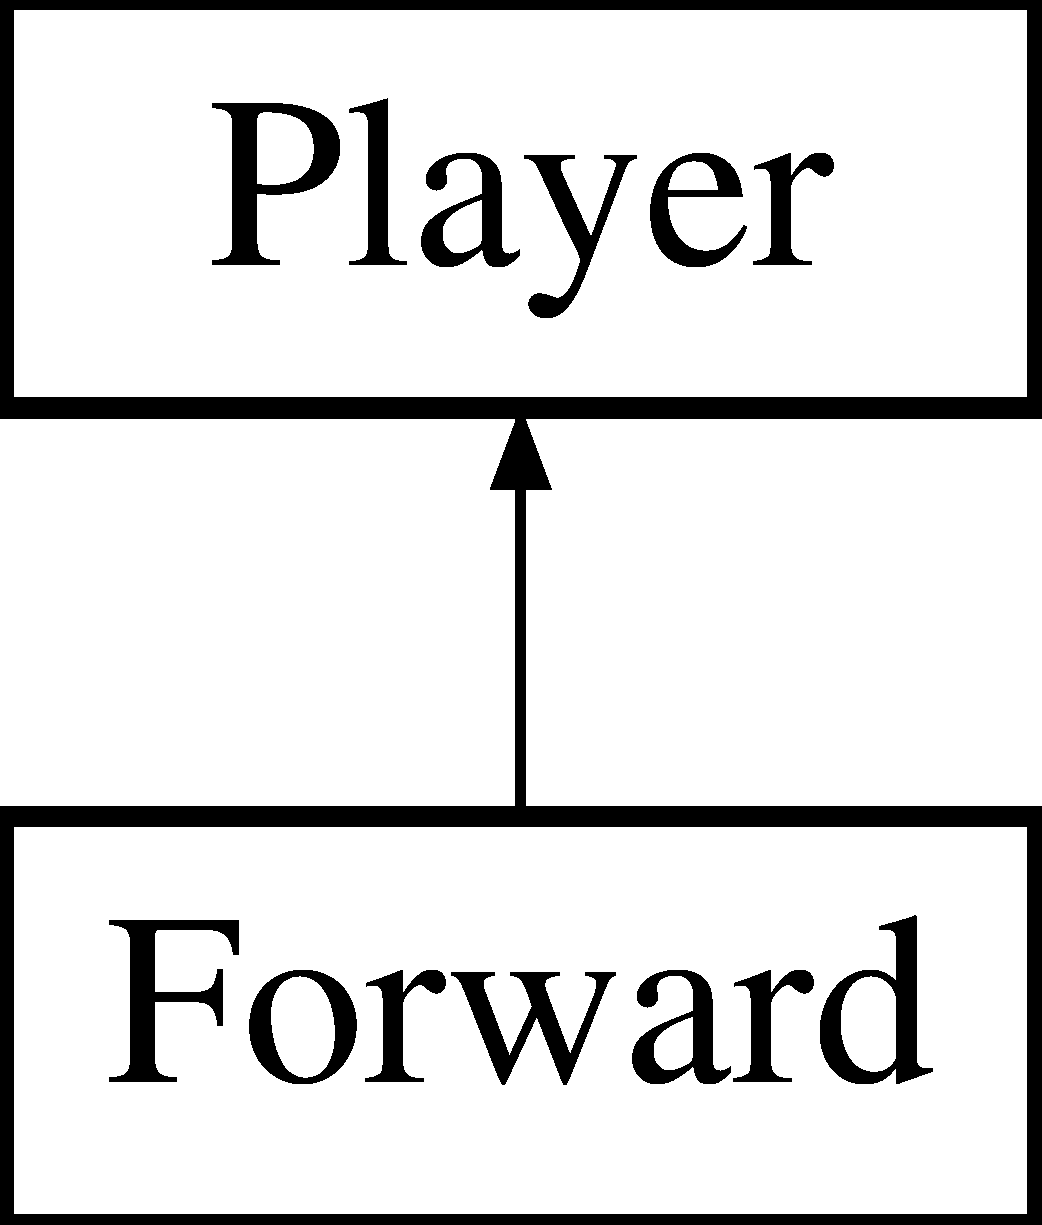
\includegraphics[height=2.000000cm]{classForward}
\end{center}
\end{figure}


\subsection{Detailed Description}
) The \hyperlink{classForward}{Forward} class inherits from the \hyperlink{classPlayer}{Player} class. The \hyperlink{classForward}{Forward} is a specialized type of \hyperlink{classPlayer}{Player} that focuses on offensive behaviors such as scoring and ball interception. 

The documentation for this class was generated from the following file:\begin{DoxyCompactItemize}
\item 
\hyperlink{Forward_8java}{Forward.java}\end{DoxyCompactItemize}

\hypertarget{classFullBack}{
\section{FullBack Class Reference}
\label{classFullBack}\index{FullBack@{FullBack}}
}
Inheritance diagram for FullBack:\begin{figure}[H]
\begin{center}
\leavevmode
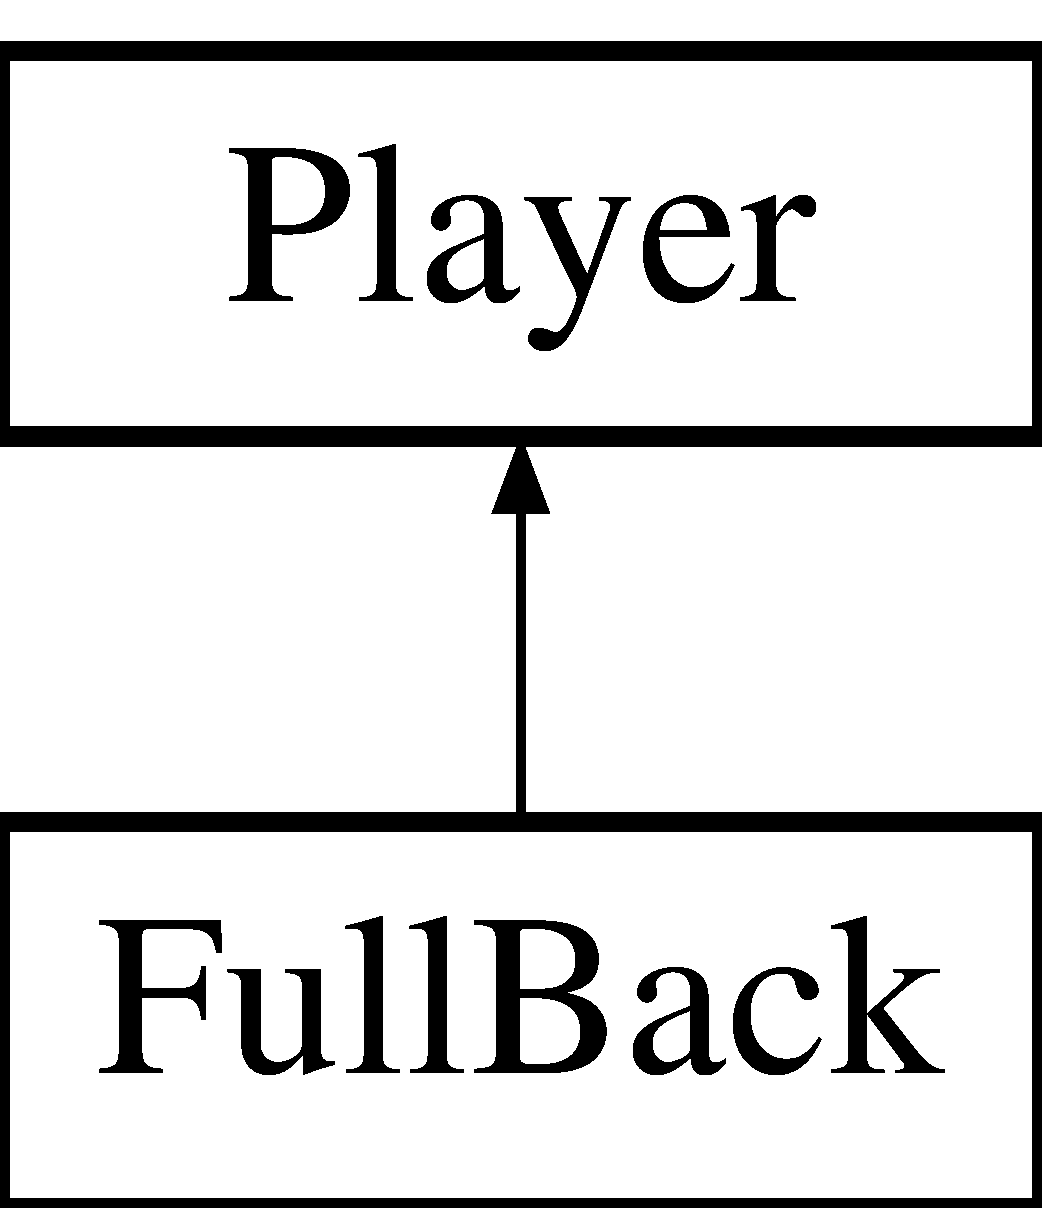
\includegraphics[height=2.000000cm]{classFullBack}
\end{center}
\end{figure}
\subsection*{Public Member Functions}
\begin{DoxyCompactItemize}
\item 
\hyperlink{classFullBack_acbe24697aec4b8fdf44d3ec60a9fa40d}{FullBack} (\hyperlink{classRoboClient}{RoboClient} rc, \hyperlink{classMemory}{Memory} m, \hyperlink{classObjInfo}{ObjInfo} i, \hyperlink{classParser}{Parser} p, int time)
\item 
\hyperlink{classFullBack_a7918587f26bf13173e7065187e48e03c}{FullBack} (String team)
\item 
void \hyperlink{classFullBack_ac213422fc423c607d56d4b5710d0192e}{initFullBack} (double x, double y)  throws SocketException, UnknownHostException 
\item 
void \hyperlink{classFullBack_a4b2e2ea2db6684474a63e7c257b9c67a}{initFullBack} (double x, double y, String pos)  throws SocketException, UnknownHostException 
\item 
\hyperlink{classObjPlayer}{ObjPlayer} \hyperlink{classFullBack_afd24e3c5ff7c8b93c77069e9f86cd9ab}{closestPlayer} ()  throws UnknownHostException, InterruptedException 
\item 
\hypertarget{classFullBack_a3638f5f61bca69dc81571c1dcbfa46e7}{
boolean {\bfseries inFullBackZone} ()}
\label{classFullBack_a3638f5f61bca69dc81571c1dcbfa46e7}

\item 
\hypertarget{classFullBack_ab02ecfe8c92fdb837ed6bf6c7389cfc0}{
void {\bfseries runDefense} ()  throws UnknownHostException, InterruptedException }
\label{classFullBack_ab02ecfe8c92fdb837ed6bf6c7389cfc0}

\item 
\hypertarget{classFullBack_aef6e79bcb91ec2baebd71a601cfe94fc}{
void {\bfseries run} ()}
\label{classFullBack_aef6e79bcb91ec2baebd71a601cfe94fc}

\end{DoxyCompactItemize}


\subsection{Detailed Description}
The \hyperlink{classFullBack}{FullBack} class inherits from the \hyperlink{classPlayer}{Player} class. The \hyperlink{classFullBack}{FullBack} is a specialized type of \hyperlink{classPlayer}{Player} that focuses on defensive behaviors such as interfering with opponent scoring. 

\subsection{Constructor \& Destructor Documentation}
\hypertarget{classFullBack_acbe24697aec4b8fdf44d3ec60a9fa40d}{
\index{FullBack@{FullBack}!FullBack@{FullBack}}
\index{FullBack@{FullBack}!FullBack@{FullBack}}
\subsubsection[{FullBack}]{\setlength{\rightskip}{0pt plus 5cm}FullBack::FullBack (
\begin{DoxyParamCaption}
\item[{{\bf RoboClient}}]{rc, }
\item[{{\bf Memory}}]{m, }
\item[{{\bf ObjInfo}}]{i, }
\item[{{\bf Parser}}]{p, }
\item[{int}]{time}
\end{DoxyParamCaption}
)\hspace{0.3cm}{\ttfamily  \mbox{[}inline\mbox{]}}}}
\label{classFullBack_acbe24697aec4b8fdf44d3ec60a9fa40d}

\begin{DoxyParams}{Parameters}
{\em rc} & \\
\hline
{\em m} & \\
\hline
{\em i} & \\
\hline
{\em p} & \\
\hline
{\em time} & \\
\hline
\end{DoxyParams}
\hypertarget{classFullBack_a7918587f26bf13173e7065187e48e03c}{
\index{FullBack@{FullBack}!FullBack@{FullBack}}
\index{FullBack@{FullBack}!FullBack@{FullBack}}
\subsubsection[{FullBack}]{\setlength{\rightskip}{0pt plus 5cm}FullBack::FullBack (
\begin{DoxyParamCaption}
\item[{String}]{team}
\end{DoxyParamCaption}
)\hspace{0.3cm}{\ttfamily  \mbox{[}inline\mbox{]}}}}
\label{classFullBack_a7918587f26bf13173e7065187e48e03c}

\begin{DoxyParams}{Parameters}
{\em team} & \\
\hline
\end{DoxyParams}


\subsection{Member Function Documentation}
\hypertarget{classFullBack_afd24e3c5ff7c8b93c77069e9f86cd9ab}{
\index{FullBack@{FullBack}!closestPlayer@{closestPlayer}}
\index{closestPlayer@{closestPlayer}!FullBack@{FullBack}}
\subsubsection[{closestPlayer}]{\setlength{\rightskip}{0pt plus 5cm}{\bf ObjPlayer} FullBack::closestPlayer (
\begin{DoxyParamCaption}
{}
\end{DoxyParamCaption}
)  throws UnknownHostException, InterruptedException \hspace{0.3cm}{\ttfamily  \mbox{[}inline\mbox{]}}}}
\label{classFullBack_afd24e3c5ff7c8b93c77069e9f86cd9ab}
Returns the closest player to the \hyperlink{classFullBack}{FullBack} on the same team. \begin{DoxyPostcond}{Postcondition}
The closest player to the \hyperlink{classFullBack}{FullBack} has been determined. 
\end{DoxyPostcond}
\begin{DoxyReturn}{Returns}
\hyperlink{classObjPlayer}{ObjPlayer} 
\end{DoxyReturn}

\begin{DoxyExceptions}{Exceptions}
{\em InterruptedException} & \\
\hline
{\em UnknownHostException} & \\
\hline
\end{DoxyExceptions}
\hypertarget{classFullBack_a4b2e2ea2db6684474a63e7c257b9c67a}{
\index{FullBack@{FullBack}!initFullBack@{initFullBack}}
\index{initFullBack@{initFullBack}!FullBack@{FullBack}}
\subsubsection[{initFullBack}]{\setlength{\rightskip}{0pt plus 5cm}void FullBack::initFullBack (
\begin{DoxyParamCaption}
\item[{double}]{x, }
\item[{double}]{y, }
\item[{String}]{pos}
\end{DoxyParamCaption}
)  throws SocketException, UnknownHostException \hspace{0.3cm}{\ttfamily  \mbox{[}inline\mbox{]}}}}
\label{classFullBack_a4b2e2ea2db6684474a63e7c257b9c67a}
Initializes the \hyperlink{classPlayer}{Player} with the RoboCup server as a goalie. \begin{DoxyPrecond}{Precondition}
A RoboCup server is available. 
\end{DoxyPrecond}
\begin{DoxyPostcond}{Postcondition}
The \hyperlink{classPlayer}{Player} has been initialized to the correct team as a goalie. 
\end{DoxyPostcond}
\hypertarget{classFullBack_ac213422fc423c607d56d4b5710d0192e}{
\index{FullBack@{FullBack}!initFullBack@{initFullBack}}
\index{initFullBack@{initFullBack}!FullBack@{FullBack}}
\subsubsection[{initFullBack}]{\setlength{\rightskip}{0pt plus 5cm}void FullBack::initFullBack (
\begin{DoxyParamCaption}
\item[{double}]{x, }
\item[{double}]{y}
\end{DoxyParamCaption}
)  throws SocketException, UnknownHostException \hspace{0.3cm}{\ttfamily  \mbox{[}inline\mbox{]}}}}
\label{classFullBack_ac213422fc423c607d56d4b5710d0192e}
Initializes the \hyperlink{classPlayer}{Player} with the RoboCup server as a goalie. \begin{DoxyPrecond}{Precondition}
A RoboCup server is available. 
\end{DoxyPrecond}
\begin{DoxyPostcond}{Postcondition}
The \hyperlink{classPlayer}{Player} has been initialized to the correct team as a goalie. 
\end{DoxyPostcond}


The documentation for this class was generated from the following file:\begin{DoxyCompactItemize}
\item 
\hyperlink{FullBack_8java}{FullBack.java}\end{DoxyCompactItemize}

\hypertarget{classFullBackBrain}{
\section{FullBackBrain Class Reference}
\label{classFullBackBrain}\index{FullBackBrain@{FullBackBrain}}
}
\subsection*{Public Member Functions}
\begin{DoxyCompactItemize}
\item 
\hyperlink{classFullBackBrain_a2a53a863ccd30fbd43b5285ec0c7b1ac}{FullBackBrain} ()
\item 
\hypertarget{classFullBackBrain_ad6645be203fec276ab293fd3b07e4759}{
{\bfseries FullBackBrain} (\hyperlink{classFullBack}{FullBack} f)}
\label{classFullBackBrain_ad6645be203fec276ab293fd3b07e4759}

\item 
\hyperlink{classAction}{Action} \hyperlink{classFullBackBrain_aac424857e8fa16dd8063a693a05fd82c}{getActions} ()
\item 
void \hyperlink{classFullBackBrain_ae0cd755da77577c80bd8fc76fe1c32f6}{setActions} (\hyperlink{classAction}{Action} actions)
\item 
\hyperlink{classFullBackBrain_a894e2167f34ee125b3b389664d1783ac}{FullBackBrain} (\hyperlink{classMode}{Mode} currentMode)
\item 
\hyperlink{classMode}{Mode} \hyperlink{classFullBackBrain_ab3fb7e8023f8e159054ccf80d1f3feca}{getCurrentMode} ()
\item 
void \hyperlink{classFullBackBrain_aa442cadff3e7304081b91d3209363fb4}{setDefensive} ()
\item 
void \hyperlink{classFullBackBrain_adc29e16b7c59d28fa182f4abb230391b}{setOffensive} ()
\item 
String \hyperlink{classFullBackBrain_a1f24e2f70fc6c841337ae6e0116811c6}{getMarked\_\-team} ()
\item 
void \hyperlink{classFullBackBrain_ac58e4c02d57b47da53bc648ef9be0bcd}{setMarked\_\-team} (String marked\_\-team)
\item 
String \hyperlink{classFullBackBrain_aa2d0607988db96aa3158258b855af250}{getMarked\_\-unum} ()
\item 
void \hyperlink{classFullBackBrain_a027bf0f42606b3be61ee79e8f6125740}{setMarked\_\-unum} (String marked\_\-unum)
\item 
void \hyperlink{classFullBackBrain_adf3bd808476349ee7aafca09a4efb86d}{run} ()
\end{DoxyCompactItemize}
\subsection*{Public Attributes}
\begin{DoxyCompactItemize}
\item 
\hypertarget{classFullBackBrain_a6817d59de2902f15ca756057e7e2089e}{
\hyperlink{classFullBack}{FullBack} {\bfseries f}}
\label{classFullBackBrain_a6817d59de2902f15ca756057e7e2089e}

\item 
\hypertarget{classFullBackBrain_a5eb89c042b9f9cba1c9cc73e2bba2ea0}{
\hyperlink{classMemory}{Memory} {\bfseries m}}
\label{classFullBackBrain_a5eb89c042b9f9cba1c9cc73e2bba2ea0}

\end{DoxyCompactItemize}


\subsection{Constructor \& Destructor Documentation}
\hypertarget{classFullBackBrain_a2a53a863ccd30fbd43b5285ec0c7b1ac}{
\index{FullBackBrain@{FullBackBrain}!FullBackBrain@{FullBackBrain}}
\index{FullBackBrain@{FullBackBrain}!FullBackBrain@{FullBackBrain}}
\subsubsection[{FullBackBrain}]{\setlength{\rightskip}{0pt plus 5cm}FullBackBrain::FullBackBrain (
\begin{DoxyParamCaption}
{}
\end{DoxyParamCaption}
)\hspace{0.3cm}{\ttfamily  \mbox{[}inline\mbox{]}}}}
\label{classFullBackBrain_a2a53a863ccd30fbd43b5285ec0c7b1ac}
Default constructor \hypertarget{classFullBackBrain_a894e2167f34ee125b3b389664d1783ac}{
\index{FullBackBrain@{FullBackBrain}!FullBackBrain@{FullBackBrain}}
\index{FullBackBrain@{FullBackBrain}!FullBackBrain@{FullBackBrain}}
\subsubsection[{FullBackBrain}]{\setlength{\rightskip}{0pt plus 5cm}FullBackBrain::FullBackBrain (
\begin{DoxyParamCaption}
\item[{{\bf Mode}}]{currentMode}
\end{DoxyParamCaption}
)\hspace{0.3cm}{\ttfamily  \mbox{[}inline\mbox{]}}}}
\label{classFullBackBrain_a894e2167f34ee125b3b389664d1783ac}
Constructor 
\begin{DoxyParams}{Parameters}
{\em currentMode} & \\
\hline
\end{DoxyParams}


\subsection{Member Function Documentation}
\hypertarget{classFullBackBrain_aac424857e8fa16dd8063a693a05fd82c}{
\index{FullBackBrain@{FullBackBrain}!getActions@{getActions}}
\index{getActions@{getActions}!FullBackBrain@{FullBackBrain}}
\subsubsection[{getActions}]{\setlength{\rightskip}{0pt plus 5cm}{\bf Action} FullBackBrain::getActions (
\begin{DoxyParamCaption}
{}
\end{DoxyParamCaption}
)\hspace{0.3cm}{\ttfamily  \mbox{[}inline\mbox{]}}}}
\label{classFullBackBrain_aac424857e8fa16dd8063a693a05fd82c}
\begin{DoxyReturn}{Returns}
the actions 
\end{DoxyReturn}
\hypertarget{classFullBackBrain_ab3fb7e8023f8e159054ccf80d1f3feca}{
\index{FullBackBrain@{FullBackBrain}!getCurrentMode@{getCurrentMode}}
\index{getCurrentMode@{getCurrentMode}!FullBackBrain@{FullBackBrain}}
\subsubsection[{getCurrentMode}]{\setlength{\rightskip}{0pt plus 5cm}{\bf Mode} FullBackBrain::getCurrentMode (
\begin{DoxyParamCaption}
{}
\end{DoxyParamCaption}
)\hspace{0.3cm}{\ttfamily  \mbox{[}inline\mbox{]}}}}
\label{classFullBackBrain_ab3fb7e8023f8e159054ccf80d1f3feca}
\begin{DoxyReturn}{Returns}
the currentMode 
\end{DoxyReturn}
\hypertarget{classFullBackBrain_a1f24e2f70fc6c841337ae6e0116811c6}{
\index{FullBackBrain@{FullBackBrain}!getMarked\_\-team@{getMarked\_\-team}}
\index{getMarked\_\-team@{getMarked\_\-team}!FullBackBrain@{FullBackBrain}}
\subsubsection[{getMarked\_\-team}]{\setlength{\rightskip}{0pt plus 5cm}String FullBackBrain::getMarked\_\-team (
\begin{DoxyParamCaption}
{}
\end{DoxyParamCaption}
)\hspace{0.3cm}{\ttfamily  \mbox{[}inline\mbox{]}}}}
\label{classFullBackBrain_a1f24e2f70fc6c841337ae6e0116811c6}
\begin{DoxyReturn}{Returns}
the marked\_\-team 
\end{DoxyReturn}
\hypertarget{classFullBackBrain_aa2d0607988db96aa3158258b855af250}{
\index{FullBackBrain@{FullBackBrain}!getMarked\_\-unum@{getMarked\_\-unum}}
\index{getMarked\_\-unum@{getMarked\_\-unum}!FullBackBrain@{FullBackBrain}}
\subsubsection[{getMarked\_\-unum}]{\setlength{\rightskip}{0pt plus 5cm}String FullBackBrain::getMarked\_\-unum (
\begin{DoxyParamCaption}
{}
\end{DoxyParamCaption}
)\hspace{0.3cm}{\ttfamily  \mbox{[}inline\mbox{]}}}}
\label{classFullBackBrain_aa2d0607988db96aa3158258b855af250}
\begin{DoxyReturn}{Returns}
the marked\_\-unum 
\end{DoxyReturn}
\hypertarget{classFullBackBrain_adf3bd808476349ee7aafca09a4efb86d}{
\index{FullBackBrain@{FullBackBrain}!run@{run}}
\index{run@{run}!FullBackBrain@{FullBackBrain}}
\subsubsection[{run}]{\setlength{\rightskip}{0pt plus 5cm}void FullBackBrain::run (
\begin{DoxyParamCaption}
{}
\end{DoxyParamCaption}
)\hspace{0.3cm}{\ttfamily  \mbox{[}inline\mbox{]}}}}
\label{classFullBackBrain_adf3bd808476349ee7aafca09a4efb86d}
The \hyperlink{classFullBackBrain}{FullBackBrain} thread run method. It instructs the \hyperlink{classFullBack}{FullBack} in soccer behaviors

\begin{DoxyPostcond}{Postcondition}
\hyperlink{classFullBack}{FullBack} will act accordingly during match. 
\end{DoxyPostcond}
\hypertarget{classFullBackBrain_ae0cd755da77577c80bd8fc76fe1c32f6}{
\index{FullBackBrain@{FullBackBrain}!setActions@{setActions}}
\index{setActions@{setActions}!FullBackBrain@{FullBackBrain}}
\subsubsection[{setActions}]{\setlength{\rightskip}{0pt plus 5cm}void FullBackBrain::setActions (
\begin{DoxyParamCaption}
\item[{{\bf Action}}]{actions}
\end{DoxyParamCaption}
)\hspace{0.3cm}{\ttfamily  \mbox{[}inline\mbox{]}}}}
\label{classFullBackBrain_ae0cd755da77577c80bd8fc76fe1c32f6}

\begin{DoxyParams}{Parameters}
{\em actions} & the actions to set \\
\hline
\end{DoxyParams}
\hypertarget{classFullBackBrain_aa442cadff3e7304081b91d3209363fb4}{
\index{FullBackBrain@{FullBackBrain}!setDefensive@{setDefensive}}
\index{setDefensive@{setDefensive}!FullBackBrain@{FullBackBrain}}
\subsubsection[{setDefensive}]{\setlength{\rightskip}{0pt plus 5cm}void FullBackBrain::setDefensive (
\begin{DoxyParamCaption}
{}
\end{DoxyParamCaption}
)\hspace{0.3cm}{\ttfamily  \mbox{[}inline\mbox{]}}}}
\label{classFullBackBrain_aa442cadff3e7304081b91d3209363fb4}
Sets the player mode to defensive \hypertarget{classFullBackBrain_ac58e4c02d57b47da53bc648ef9be0bcd}{
\index{FullBackBrain@{FullBackBrain}!setMarked\_\-team@{setMarked\_\-team}}
\index{setMarked\_\-team@{setMarked\_\-team}!FullBackBrain@{FullBackBrain}}
\subsubsection[{setMarked\_\-team}]{\setlength{\rightskip}{0pt plus 5cm}void FullBackBrain::setMarked\_\-team (
\begin{DoxyParamCaption}
\item[{String}]{marked\_\-team}
\end{DoxyParamCaption}
)\hspace{0.3cm}{\ttfamily  \mbox{[}inline\mbox{]}}}}
\label{classFullBackBrain_ac58e4c02d57b47da53bc648ef9be0bcd}

\begin{DoxyParams}{Parameters}
{\em marked\_\-team} & the marked\_\-team to set \\
\hline
\end{DoxyParams}
\hypertarget{classFullBackBrain_a027bf0f42606b3be61ee79e8f6125740}{
\index{FullBackBrain@{FullBackBrain}!setMarked\_\-unum@{setMarked\_\-unum}}
\index{setMarked\_\-unum@{setMarked\_\-unum}!FullBackBrain@{FullBackBrain}}
\subsubsection[{setMarked\_\-unum}]{\setlength{\rightskip}{0pt plus 5cm}void FullBackBrain::setMarked\_\-unum (
\begin{DoxyParamCaption}
\item[{String}]{marked\_\-unum}
\end{DoxyParamCaption}
)\hspace{0.3cm}{\ttfamily  \mbox{[}inline\mbox{]}}}}
\label{classFullBackBrain_a027bf0f42606b3be61ee79e8f6125740}

\begin{DoxyParams}{Parameters}
{\em marked\_\-unum} & the marked\_\-unum to set \\
\hline
\end{DoxyParams}
\hypertarget{classFullBackBrain_adc29e16b7c59d28fa182f4abb230391b}{
\index{FullBackBrain@{FullBackBrain}!setOffensive@{setOffensive}}
\index{setOffensive@{setOffensive}!FullBackBrain@{FullBackBrain}}
\subsubsection[{setOffensive}]{\setlength{\rightskip}{0pt plus 5cm}void FullBackBrain::setOffensive (
\begin{DoxyParamCaption}
{}
\end{DoxyParamCaption}
)\hspace{0.3cm}{\ttfamily  \mbox{[}inline\mbox{]}}}}
\label{classFullBackBrain_adc29e16b7c59d28fa182f4abb230391b}
Sets the player mode to be offensive 

The documentation for this class was generated from the following file:\begin{DoxyCompactItemize}
\item 
FullBackBrain.java\end{DoxyCompactItemize}

\hypertarget{classGame}{
\section{Game Class Reference}
\label{classGame}\index{Game@{Game}}
}
\subsection*{Static Public Member Functions}
\begin{DoxyCompactItemize}
\item 
\hypertarget{classGame_a3320680a7bc7941aed1594a923181205}{
static void {\bfseries main} (String args\mbox{[}$\,$\mbox{]})  throws Exception 	}
\label{classGame_a3320680a7bc7941aed1594a923181205}

\end{DoxyCompactItemize}


\subsection{Detailed Description}
This serves as a main class to assemble the RoboCup team and set them into action for the match. 

The documentation for this class was generated from the following file:\begin{DoxyCompactItemize}
\item 
\hyperlink{Game_8java}{Game.java}\end{DoxyCompactItemize}

\hypertarget{classGoalie}{
\section{Goalie Class Reference}
\label{classGoalie}\index{Goalie@{Goalie}}
}
Inheritance diagram for Goalie:\begin{figure}[H]
\begin{center}
\leavevmode
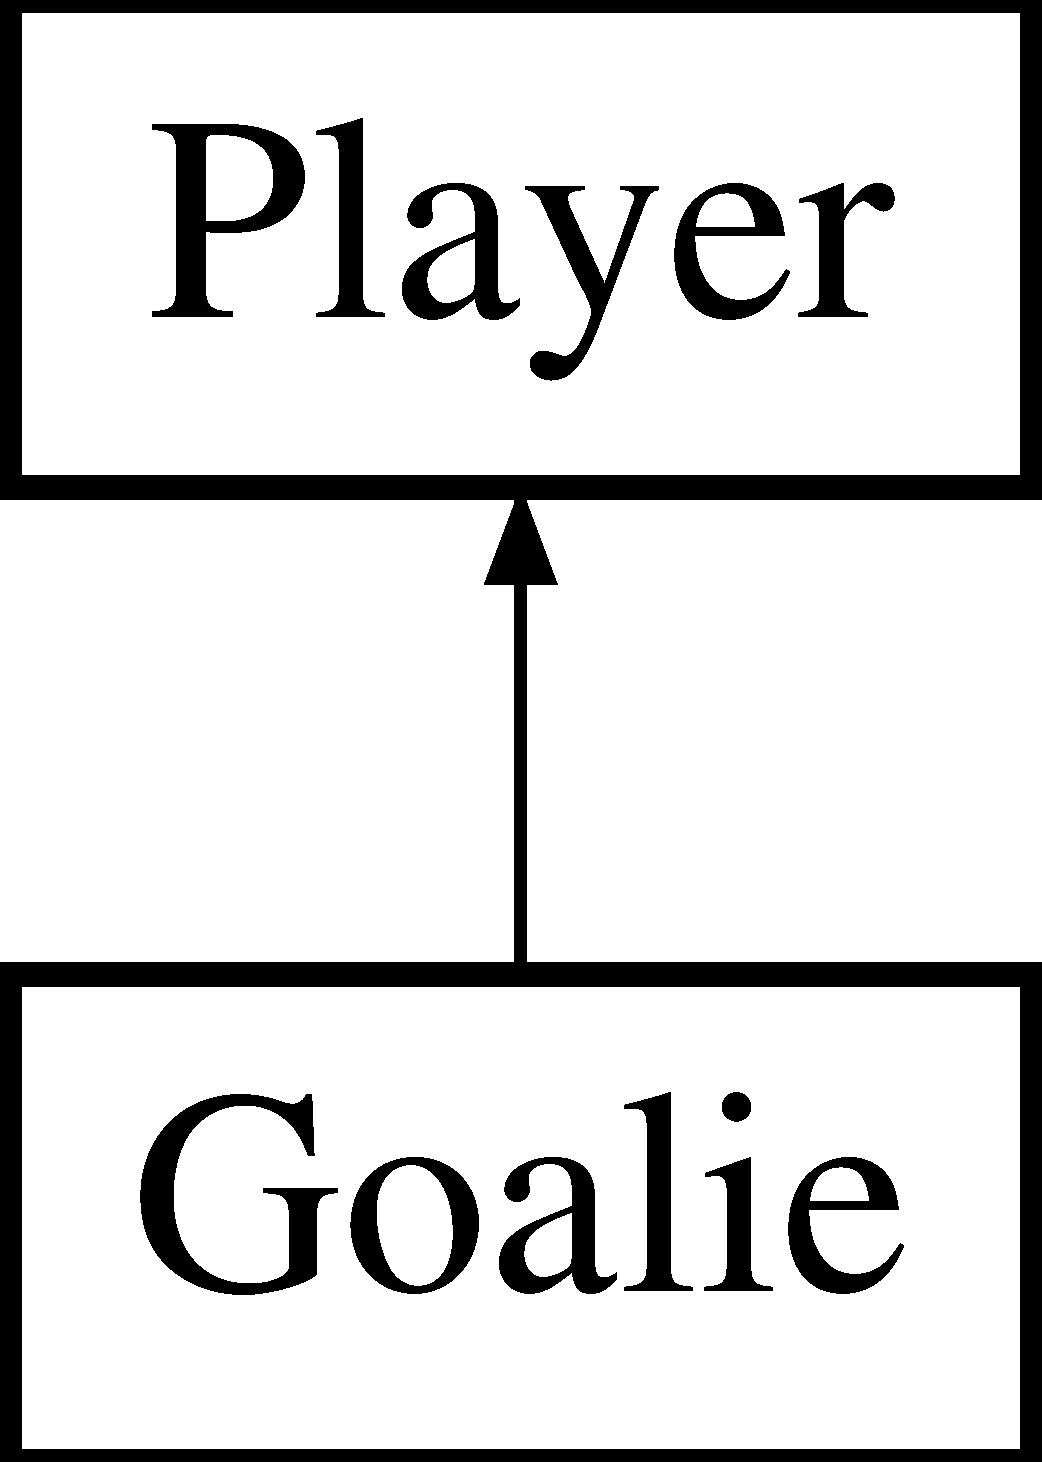
\includegraphics[height=2.000000cm]{classGoalie}
\end{center}
\end{figure}
\subsection*{Public Member Functions}
\begin{DoxyCompactItemize}
\item 
\hypertarget{classGoalie_a61f0e1513d23a5bfd8b06b4f64485f14}{
{\bfseries Goalie} (String team)}
\label{classGoalie_a61f0e1513d23a5bfd8b06b4f64485f14}

\item 
void \hyperlink{classGoalie_ad20be55693ae031a73e703960ae96db3}{initGoalie} (double x, double y)  throws SocketException, UnknownHostException 
\item 
void \hyperlink{classGoalie_aa31abfeafaa76d73433c75661e9ee214}{catchball} (double d)  throws UnknownHostException
\item 
void \hyperlink{classGoalie_a6fa9af8f62836e180e56a51f9bc126dc}{followBall} ()
\item 
boolean \hyperlink{classGoalie_aeedb27a3d7123889aa35b122cd9f8e6a}{ballInGoalzone} (\hyperlink{classObjBall}{ObjBall} ball)
\item 
boolean \hyperlink{classGoalie_aff96bcc0763bcb7ca922beae5f6f7f6f}{catchable} ()
\item 
void \hyperlink{classGoalie_a3d00b5dcb6db3925a8eeaf667a2f1650}{defendGoal} (\hyperlink{classObjBall}{ObjBall} ball)  throws UnknownHostException, InterruptedException 
\item 
void \hyperlink{classGoalie_a6b24e53882b2d38ca452c263eb9c58cd}{positionGoalie} (\hyperlink{classObjBall}{ObjBall} ball)  throws InterruptedException 
\item 
void \hyperlink{classGoalie_aacefd54603f62188922344f027a60b65}{getBtwBallAndGoal} (\hyperlink{classObjBall}{ObjBall} ball)
\item 
\hyperlink{classObjPlayer}{ObjPlayer} \hyperlink{classGoalie_a1377353efede128a3367bde1e8b4137a}{closestPlayer} ()  throws UnknownHostException, InterruptedException 
\item 
void \hyperlink{classGoalie_acef3607fe805cab95fe5c51319b6d858}{kickToPlayer} (\hyperlink{classObjPlayer}{ObjPlayer} player)
\item 
void \hyperlink{classGoalie_a4fc1cb6aef2b752d6eaf198b33355ba3}{kickBallOutOfBounds} ()
\item 
\hypertarget{classGoalie_a4746e13da625b6794aab143d8c3bf12f}{
void {\bfseries run} ()}
\label{classGoalie_a4746e13da625b6794aab143d8c3bf12f}

\end{DoxyCompactItemize}
\subsection*{Public Attributes}
\begin{DoxyCompactItemize}
\item 
\hypertarget{classGoalie_a30191095e1d0cfb3309d7776d2f1b91d}{
boolean {\bfseries ballTurn} = false}
\label{classGoalie_a30191095e1d0cfb3309d7776d2f1b91d}

\item 
\hypertarget{classGoalie_aa14c124f0012e6bf819efaa138597dbb}{
\hyperlink{classMathHelp}{MathHelp} {\bfseries mh} = new \hyperlink{classMathHelp}{MathHelp}()}
\label{classGoalie_aa14c124f0012e6bf819efaa138597dbb}

\end{DoxyCompactItemize}
\subsection*{Package Attributes}
\begin{DoxyCompactItemize}
\item 
\hypertarget{classGoalie_adc308adc44b3cfca5df2cdd7bb212c9e}{
boolean {\bfseries ballCaught} = false}
\label{classGoalie_adc308adc44b3cfca5df2cdd7bb212c9e}

\end{DoxyCompactItemize}


\subsection{Detailed Description}
The \hyperlink{classGoalie}{Goalie} class inherits from the \hyperlink{classPlayer}{Player} class. The \hyperlink{classGoalie}{Goalie} is a specialized type of \hyperlink{classPlayer}{Player} that may catch the ball under certain conditions and defends the goal from the opposing team. 

\subsection{Member Function Documentation}
\hypertarget{classGoalie_aeedb27a3d7123889aa35b122cd9f8e6a}{
\index{Goalie@{Goalie}!ballInGoalzone@{ballInGoalzone}}
\index{ballInGoalzone@{ballInGoalzone}!Goalie@{Goalie}}
\subsubsection[{ballInGoalzone}]{\setlength{\rightskip}{0pt plus 5cm}boolean Goalie::ballInGoalzone (
\begin{DoxyParamCaption}
\item[{{\bf ObjBall}}]{ball}
\end{DoxyParamCaption}
)\hspace{0.3cm}{\ttfamily  \mbox{[}inline\mbox{]}}}}
\label{classGoalie_aeedb27a3d7123889aa35b122cd9f8e6a}
A method to determine whether the ball is in the penalty box


\begin{DoxyParams}{Parameters}
{\em ball} & the \hyperlink{classObjBall}{ObjBall} to follow \\
\hline
\end{DoxyParams}
\begin{DoxyPrecond}{Precondition}
this must be called with an \hyperlink{classObjBall}{ObjBall} 
\end{DoxyPrecond}
\begin{DoxyPostcond}{Postcondition}
true if ball is in penalty box, false if it's not 
\end{DoxyPostcond}
\begin{DoxyReturn}{Returns}
boolean 
\end{DoxyReturn}
\hypertarget{classGoalie_aff96bcc0763bcb7ca922beae5f6f7f6f}{
\index{Goalie@{Goalie}!catchable@{catchable}}
\index{catchable@{catchable}!Goalie@{Goalie}}
\subsubsection[{catchable}]{\setlength{\rightskip}{0pt plus 5cm}boolean Goalie::catchable (
\begin{DoxyParamCaption}
{}
\end{DoxyParamCaption}
)\hspace{0.3cm}{\ttfamily  \mbox{[}inline\mbox{]}}}}
\label{classGoalie_aff96bcc0763bcb7ca922beae5f6f7f6f}
Returns true or false depending on whether the ball is within the catchable range of the goalie. \begin{DoxyPrecond}{Precondition}
The ball is visible to the goalie 
\end{DoxyPrecond}
\begin{DoxyPostcond}{Postcondition}
The ball is determined to catchable or not. 
\end{DoxyPostcond}
\begin{DoxyReturn}{Returns}
boolean True if catchable, false if not. 
\end{DoxyReturn}
\hypertarget{classGoalie_aa31abfeafaa76d73433c75661e9ee214}{
\index{Goalie@{Goalie}!catchball@{catchball}}
\index{catchball@{catchball}!Goalie@{Goalie}}
\subsubsection[{catchball}]{\setlength{\rightskip}{0pt plus 5cm}void Goalie::catchball (
\begin{DoxyParamCaption}
\item[{double}]{d}
\end{DoxyParamCaption}
)  throws UnknownHostException\hspace{0.3cm}{\ttfamily  \mbox{[}inline\mbox{]}}}}
\label{classGoalie_aa31abfeafaa76d73433c75661e9ee214}
Causes the \hyperlink{classGoalie}{Goalie} to catch the ball. \begin{DoxyPrecond}{Precondition}
Playmode is play-\/on, ball is within goalkeeper zone and in the catchable area. 
\end{DoxyPrecond}
\begin{DoxyPostcond}{Postcondition}
The \hyperlink{classGoalie}{Goalie} has caught the ball. 
\end{DoxyPostcond}
\hypertarget{classGoalie_a1377353efede128a3367bde1e8b4137a}{
\index{Goalie@{Goalie}!closestPlayer@{closestPlayer}}
\index{closestPlayer@{closestPlayer}!Goalie@{Goalie}}
\subsubsection[{closestPlayer}]{\setlength{\rightskip}{0pt plus 5cm}{\bf ObjPlayer} Goalie::closestPlayer (
\begin{DoxyParamCaption}
{}
\end{DoxyParamCaption}
)  throws UnknownHostException, InterruptedException \hspace{0.3cm}{\ttfamily  \mbox{[}inline\mbox{]}}}}
\label{classGoalie_a1377353efede128a3367bde1e8b4137a}
Returns the closest player to the goalie on the same team. \begin{DoxyPostcond}{Postcondition}
The closest player to the goalie has been determined. 
\end{DoxyPostcond}
\begin{DoxyReturn}{Returns}
\hyperlink{classObjPlayer}{ObjPlayer} 
\end{DoxyReturn}

\begin{DoxyExceptions}{Exceptions}
{\em InterruptedException} & \\
\hline
{\em UnknownHostException} & \\
\hline
\end{DoxyExceptions}
\hypertarget{classGoalie_a3d00b5dcb6db3925a8eeaf667a2f1650}{
\index{Goalie@{Goalie}!defendGoal@{defendGoal}}
\index{defendGoal@{defendGoal}!Goalie@{Goalie}}
\subsubsection[{defendGoal}]{\setlength{\rightskip}{0pt plus 5cm}void Goalie::defendGoal (
\begin{DoxyParamCaption}
\item[{{\bf ObjBall}}]{ball}
\end{DoxyParamCaption}
)  throws UnknownHostException, InterruptedException \hspace{0.3cm}{\ttfamily  \mbox{[}inline\mbox{]}}}}
\label{classGoalie_a3d00b5dcb6db3925a8eeaf667a2f1650}
Causes the goalie to act to intercept the ball as it approaches the goal. 
\begin{DoxyParams}{Parameters}
{\em \hyperlink{classObjBall}{ObjBall}} & representing the ball in play. \\
\hline
\end{DoxyParams}

\begin{DoxyExceptions}{Exceptions}
{\em UnknownHostException} & \\
\hline
{\em InterruptedException} & \\
\hline
\end{DoxyExceptions}
\begin{DoxyPrecond}{Precondition}
The ball has entered the goal zone. 
\end{DoxyPrecond}
\begin{DoxyPostcond}{Postcondition}
The ball has been caught by the goalie, or the goalie has missed the ball. 
\end{DoxyPostcond}
\hypertarget{classGoalie_a6fa9af8f62836e180e56a51f9bc126dc}{
\index{Goalie@{Goalie}!followBall@{followBall}}
\index{followBall@{followBall}!Goalie@{Goalie}}
\subsubsection[{followBall}]{\setlength{\rightskip}{0pt plus 5cm}void Goalie::followBall (
\begin{DoxyParamCaption}
{}
\end{DoxyParamCaption}
)\hspace{0.3cm}{\ttfamily  \mbox{[}inline\mbox{]}}}}
\label{classGoalie_a6fa9af8f62836e180e56a51f9bc126dc}
Turns goalie toward the ball \begin{DoxyPostcond}{Postcondition}
The goalie will turn in the direction of the ball 
\end{DoxyPostcond}
\hypertarget{classGoalie_aacefd54603f62188922344f027a60b65}{
\index{Goalie@{Goalie}!getBtwBallAndGoal@{getBtwBallAndGoal}}
\index{getBtwBallAndGoal@{getBtwBallAndGoal}!Goalie@{Goalie}}
\subsubsection[{getBtwBallAndGoal}]{\setlength{\rightskip}{0pt plus 5cm}void Goalie::getBtwBallAndGoal (
\begin{DoxyParamCaption}
\item[{{\bf ObjBall}}]{ball}
\end{DoxyParamCaption}
)\hspace{0.3cm}{\ttfamily  \mbox{[}inline\mbox{]}}}}
\label{classGoalie_aacefd54603f62188922344f027a60b65}
Moves goalie between the ball and the goal (under construction) 
\begin{DoxyParams}{Parameters}
{\em ball} & An \hyperlink{classObjBall}{ObjBall}. \\
\hline
\end{DoxyParams}
\begin{DoxyPrecond}{Precondition}
Ball is visible to the goalie. 
\end{DoxyPrecond}
\begin{DoxyPostcond}{Postcondition}
The goalie has moved to a point on the line between the ball and the goal. 
\end{DoxyPostcond}
\hypertarget{classGoalie_ad20be55693ae031a73e703960ae96db3}{
\index{Goalie@{Goalie}!initGoalie@{initGoalie}}
\index{initGoalie@{initGoalie}!Goalie@{Goalie}}
\subsubsection[{initGoalie}]{\setlength{\rightskip}{0pt plus 5cm}void Goalie::initGoalie (
\begin{DoxyParamCaption}
\item[{double}]{x, }
\item[{double}]{y}
\end{DoxyParamCaption}
)  throws SocketException, UnknownHostException \hspace{0.3cm}{\ttfamily  \mbox{[}inline\mbox{]}}}}
\label{classGoalie_ad20be55693ae031a73e703960ae96db3}
Initializes the \hyperlink{classPlayer}{Player} with the RoboCup server as a goalie. \begin{DoxyPrecond}{Precondition}
A RoboCup server is available. 
\end{DoxyPrecond}
\begin{DoxyPostcond}{Postcondition}
The \hyperlink{classPlayer}{Player} has been initialized to the correct team as a goalie. 
\end{DoxyPostcond}
\hypertarget{classGoalie_a4fc1cb6aef2b752d6eaf198b33355ba3}{
\index{Goalie@{Goalie}!kickBallOutOfBounds@{kickBallOutOfBounds}}
\index{kickBallOutOfBounds@{kickBallOutOfBounds}!Goalie@{Goalie}}
\subsubsection[{kickBallOutOfBounds}]{\setlength{\rightskip}{0pt plus 5cm}void Goalie::kickBallOutOfBounds (
\begin{DoxyParamCaption}
{}
\end{DoxyParamCaption}
)\hspace{0.3cm}{\ttfamily  \mbox{[}inline\mbox{]}}}}
\label{classGoalie_a4fc1cb6aef2b752d6eaf198b33355ba3}
Causes the goalie to kick the ball out of bounds (Currently unused.) \begin{DoxyPrecond}{Precondition}
\hyperlink{classGoalie}{Goalie} has control of the ball 
\end{DoxyPrecond}
\begin{DoxyPostcond}{Postcondition}
Ball has been kicked out of bounds 
\end{DoxyPostcond}
\hypertarget{classGoalie_acef3607fe805cab95fe5c51319b6d858}{
\index{Goalie@{Goalie}!kickToPlayer@{kickToPlayer}}
\index{kickToPlayer@{kickToPlayer}!Goalie@{Goalie}}
\subsubsection[{kickToPlayer}]{\setlength{\rightskip}{0pt plus 5cm}void Goalie::kickToPlayer (
\begin{DoxyParamCaption}
\item[{{\bf ObjPlayer}}]{player}
\end{DoxyParamCaption}
)\hspace{0.3cm}{\ttfamily  \mbox{[}inline\mbox{]}}}}
\label{classGoalie_acef3607fe805cab95fe5c51319b6d858}
Causes goalie to kick the ball to a specific player. (Currently unused.) \begin{DoxyPrecond}{Precondition}
A player is in sight of the goalie. 
\end{DoxyPrecond}
\begin{DoxyPostcond}{Postcondition}
The goalie has kicked the ball to the player passed to the function. 
\end{DoxyPostcond}

\begin{DoxyParams}{Parameters}
{\em player} & An \hyperlink{classObjPlayer}{ObjPlayer} representing the player to receive the ball. \\
\hline
\end{DoxyParams}
\hypertarget{classGoalie_a6b24e53882b2d38ca452c263eb9c58cd}{
\index{Goalie@{Goalie}!positionGoalie@{positionGoalie}}
\index{positionGoalie@{positionGoalie}!Goalie@{Goalie}}
\subsubsection[{positionGoalie}]{\setlength{\rightskip}{0pt plus 5cm}void Goalie::positionGoalie (
\begin{DoxyParamCaption}
\item[{{\bf ObjBall}}]{ball}
\end{DoxyParamCaption}
)  throws InterruptedException \hspace{0.3cm}{\ttfamily  \mbox{[}inline\mbox{]}}}}
\label{classGoalie_a6b24e53882b2d38ca452c263eb9c58cd}
Moves goalie to specific points within the goalbox dependent upon where the ball is on the field. 
\begin{DoxyParams}{Parameters}
{\em ball} & An \hyperlink{classObjBall}{ObjBall} representing the ball in play. \\
\hline
\end{DoxyParams}

\begin{DoxyExceptions}{Exceptions}
{\em InterruptedException} & \\
\hline
\end{DoxyExceptions}
\begin{DoxyPrecond}{Precondition}
The ball is visible. 
\end{DoxyPrecond}
\begin{DoxyPostcond}{Postcondition}
The goalie has moved to a strategic position to get between the ball and the goal. 
\end{DoxyPostcond}


The documentation for this class was generated from the following file:\begin{DoxyCompactItemize}
\item 
\hyperlink{Goalie_8java}{Goalie.java}\end{DoxyCompactItemize}

\hypertarget{classGoalieBrain}{
\section{GoalieBrain Class Reference}
\label{classGoalieBrain}\index{GoalieBrain@{GoalieBrain}}
}
\subsection*{Public Member Functions}
\begin{DoxyCompactItemize}
\item 
\hyperlink{classGoalieBrain_ab41953290ee4a03022065b61cfa1fcf8}{GoalieBrain} ()
\item 
\hypertarget{classGoalieBrain_afcd5b30d276f2f1bdeaf487275a50dc4}{
{\bfseries GoalieBrain} (\hyperlink{classGoalie}{Goalie} g)}
\label{classGoalieBrain_afcd5b30d276f2f1bdeaf487275a50dc4}

\item 
\hyperlink{classAction}{Action} \hyperlink{classGoalieBrain_ae07a39e4385196b62ee791cb43b0fe57}{getActions} ()
\item 
void \hyperlink{classGoalieBrain_a6c696c9b123c07ebaaf1fa072357278b}{setActions} (\hyperlink{classAction}{Action} actions)
\item 
\hyperlink{classGoalieBrain_a404c279dd38842abe9774eeff7bb56a0}{GoalieBrain} (\hyperlink{classMode}{Mode} currentMode)
\item 
\hyperlink{classMode}{Mode} \hyperlink{classGoalieBrain_a72c84bb51ce2d78948dbb500ba9d37f6}{getCurrentMode} ()
\item 
void \hyperlink{classGoalieBrain_ac48806ea1347f6f19618c701e501e693}{setDefensive} ()
\item 
void \hyperlink{classGoalieBrain_a72bd08064a4bd4d7880c75b7cec094c1}{setOffensive} ()
\item 
String \hyperlink{classGoalieBrain_a0c1501fa8e12dd8317e2f6d19bc0dfcf}{getMarked\_\-team} ()
\item 
void \hyperlink{classGoalieBrain_a84d421b2692c1c322cdabb8cd746ab66}{setMarked\_\-team} (String marked\_\-team)
\item 
String \hyperlink{classGoalieBrain_ab4b67d9834099cfc0a3c1edfcd7da379}{getMarked\_\-unum} ()
\item 
void \hyperlink{classGoalieBrain_ab4ed70b7ff134d18c4975af6ec91dbff}{setMarked\_\-unum} (String marked\_\-unum)
\item 
void \hyperlink{classGoalieBrain_a5a680f40c458b231d21473fd397cd448}{run} ()
\end{DoxyCompactItemize}
\subsection*{Public Attributes}
\begin{DoxyCompactItemize}
\item 
\hypertarget{classGoalieBrain_a43a238dc39a7af4800d087a331e24d7b}{
\hyperlink{classGoalie}{Goalie} {\bfseries g}}
\label{classGoalieBrain_a43a238dc39a7af4800d087a331e24d7b}

\item 
\hypertarget{classGoalieBrain_aed346f9b8ebb10dd6f820f2570898a71}{
\hyperlink{classMemory}{Memory} {\bfseries m}}
\label{classGoalieBrain_aed346f9b8ebb10dd6f820f2570898a71}

\end{DoxyCompactItemize}


\subsection{Constructor \& Destructor Documentation}
\hypertarget{classGoalieBrain_ab41953290ee4a03022065b61cfa1fcf8}{
\index{GoalieBrain@{GoalieBrain}!GoalieBrain@{GoalieBrain}}
\index{GoalieBrain@{GoalieBrain}!GoalieBrain@{GoalieBrain}}
\subsubsection[{GoalieBrain}]{\setlength{\rightskip}{0pt plus 5cm}GoalieBrain::GoalieBrain (
\begin{DoxyParamCaption}
{}
\end{DoxyParamCaption}
)\hspace{0.3cm}{\ttfamily  \mbox{[}inline\mbox{]}}}}
\label{classGoalieBrain_ab41953290ee4a03022065b61cfa1fcf8}
Default constructor \hypertarget{classGoalieBrain_a404c279dd38842abe9774eeff7bb56a0}{
\index{GoalieBrain@{GoalieBrain}!GoalieBrain@{GoalieBrain}}
\index{GoalieBrain@{GoalieBrain}!GoalieBrain@{GoalieBrain}}
\subsubsection[{GoalieBrain}]{\setlength{\rightskip}{0pt plus 5cm}GoalieBrain::GoalieBrain (
\begin{DoxyParamCaption}
\item[{{\bf Mode}}]{currentMode}
\end{DoxyParamCaption}
)\hspace{0.3cm}{\ttfamily  \mbox{[}inline\mbox{]}}}}
\label{classGoalieBrain_a404c279dd38842abe9774eeff7bb56a0}
Constructor 
\begin{DoxyParams}{Parameters}
{\em currentMode} & \\
\hline
\end{DoxyParams}


\subsection{Member Function Documentation}
\hypertarget{classGoalieBrain_ae07a39e4385196b62ee791cb43b0fe57}{
\index{GoalieBrain@{GoalieBrain}!getActions@{getActions}}
\index{getActions@{getActions}!GoalieBrain@{GoalieBrain}}
\subsubsection[{getActions}]{\setlength{\rightskip}{0pt plus 5cm}{\bf Action} GoalieBrain::getActions (
\begin{DoxyParamCaption}
{}
\end{DoxyParamCaption}
)\hspace{0.3cm}{\ttfamily  \mbox{[}inline\mbox{]}}}}
\label{classGoalieBrain_ae07a39e4385196b62ee791cb43b0fe57}
\begin{DoxyReturn}{Returns}
the actions 
\end{DoxyReturn}
\hypertarget{classGoalieBrain_a72c84bb51ce2d78948dbb500ba9d37f6}{
\index{GoalieBrain@{GoalieBrain}!getCurrentMode@{getCurrentMode}}
\index{getCurrentMode@{getCurrentMode}!GoalieBrain@{GoalieBrain}}
\subsubsection[{getCurrentMode}]{\setlength{\rightskip}{0pt plus 5cm}{\bf Mode} GoalieBrain::getCurrentMode (
\begin{DoxyParamCaption}
{}
\end{DoxyParamCaption}
)\hspace{0.3cm}{\ttfamily  \mbox{[}inline\mbox{]}}}}
\label{classGoalieBrain_a72c84bb51ce2d78948dbb500ba9d37f6}
\begin{DoxyReturn}{Returns}
the currentMode 
\end{DoxyReturn}
\hypertarget{classGoalieBrain_a0c1501fa8e12dd8317e2f6d19bc0dfcf}{
\index{GoalieBrain@{GoalieBrain}!getMarked\_\-team@{getMarked\_\-team}}
\index{getMarked\_\-team@{getMarked\_\-team}!GoalieBrain@{GoalieBrain}}
\subsubsection[{getMarked\_\-team}]{\setlength{\rightskip}{0pt plus 5cm}String GoalieBrain::getMarked\_\-team (
\begin{DoxyParamCaption}
{}
\end{DoxyParamCaption}
)\hspace{0.3cm}{\ttfamily  \mbox{[}inline\mbox{]}}}}
\label{classGoalieBrain_a0c1501fa8e12dd8317e2f6d19bc0dfcf}
\begin{DoxyReturn}{Returns}
the marked\_\-team 
\end{DoxyReturn}
\hypertarget{classGoalieBrain_ab4b67d9834099cfc0a3c1edfcd7da379}{
\index{GoalieBrain@{GoalieBrain}!getMarked\_\-unum@{getMarked\_\-unum}}
\index{getMarked\_\-unum@{getMarked\_\-unum}!GoalieBrain@{GoalieBrain}}
\subsubsection[{getMarked\_\-unum}]{\setlength{\rightskip}{0pt plus 5cm}String GoalieBrain::getMarked\_\-unum (
\begin{DoxyParamCaption}
{}
\end{DoxyParamCaption}
)\hspace{0.3cm}{\ttfamily  \mbox{[}inline\mbox{]}}}}
\label{classGoalieBrain_ab4b67d9834099cfc0a3c1edfcd7da379}
\begin{DoxyReturn}{Returns}
the marked\_\-unum 
\end{DoxyReturn}
\hypertarget{classGoalieBrain_a5a680f40c458b231d21473fd397cd448}{
\index{GoalieBrain@{GoalieBrain}!run@{run}}
\index{run@{run}!GoalieBrain@{GoalieBrain}}
\subsubsection[{run}]{\setlength{\rightskip}{0pt plus 5cm}void GoalieBrain::run (
\begin{DoxyParamCaption}
{}
\end{DoxyParamCaption}
)\hspace{0.3cm}{\ttfamily  \mbox{[}inline\mbox{]}}}}
\label{classGoalieBrain_a5a680f40c458b231d21473fd397cd448}
The \hyperlink{classBrain}{Brain} thread run method. It causes the \hyperlink{classGoalie}{Goalie} to exhibit soccer behaviors.

\begin{DoxyPostcond}{Postcondition}
\hyperlink{classGoalie}{Goalie} will perform \hyperlink{classGoalie}{Goalie} functions during match. 
\end{DoxyPostcond}
\hypertarget{classGoalieBrain_a6c696c9b123c07ebaaf1fa072357278b}{
\index{GoalieBrain@{GoalieBrain}!setActions@{setActions}}
\index{setActions@{setActions}!GoalieBrain@{GoalieBrain}}
\subsubsection[{setActions}]{\setlength{\rightskip}{0pt plus 5cm}void GoalieBrain::setActions (
\begin{DoxyParamCaption}
\item[{{\bf Action}}]{actions}
\end{DoxyParamCaption}
)\hspace{0.3cm}{\ttfamily  \mbox{[}inline\mbox{]}}}}
\label{classGoalieBrain_a6c696c9b123c07ebaaf1fa072357278b}

\begin{DoxyParams}{Parameters}
{\em actions} & the actions to set \\
\hline
\end{DoxyParams}
\hypertarget{classGoalieBrain_ac48806ea1347f6f19618c701e501e693}{
\index{GoalieBrain@{GoalieBrain}!setDefensive@{setDefensive}}
\index{setDefensive@{setDefensive}!GoalieBrain@{GoalieBrain}}
\subsubsection[{setDefensive}]{\setlength{\rightskip}{0pt plus 5cm}void GoalieBrain::setDefensive (
\begin{DoxyParamCaption}
{}
\end{DoxyParamCaption}
)\hspace{0.3cm}{\ttfamily  \mbox{[}inline\mbox{]}}}}
\label{classGoalieBrain_ac48806ea1347f6f19618c701e501e693}
Sets the player mode to defensive \hypertarget{classGoalieBrain_a84d421b2692c1c322cdabb8cd746ab66}{
\index{GoalieBrain@{GoalieBrain}!setMarked\_\-team@{setMarked\_\-team}}
\index{setMarked\_\-team@{setMarked\_\-team}!GoalieBrain@{GoalieBrain}}
\subsubsection[{setMarked\_\-team}]{\setlength{\rightskip}{0pt plus 5cm}void GoalieBrain::setMarked\_\-team (
\begin{DoxyParamCaption}
\item[{String}]{marked\_\-team}
\end{DoxyParamCaption}
)\hspace{0.3cm}{\ttfamily  \mbox{[}inline\mbox{]}}}}
\label{classGoalieBrain_a84d421b2692c1c322cdabb8cd746ab66}

\begin{DoxyParams}{Parameters}
{\em marked\_\-team} & the marked\_\-team to set \\
\hline
\end{DoxyParams}
\hypertarget{classGoalieBrain_ab4ed70b7ff134d18c4975af6ec91dbff}{
\index{GoalieBrain@{GoalieBrain}!setMarked\_\-unum@{setMarked\_\-unum}}
\index{setMarked\_\-unum@{setMarked\_\-unum}!GoalieBrain@{GoalieBrain}}
\subsubsection[{setMarked\_\-unum}]{\setlength{\rightskip}{0pt plus 5cm}void GoalieBrain::setMarked\_\-unum (
\begin{DoxyParamCaption}
\item[{String}]{marked\_\-unum}
\end{DoxyParamCaption}
)\hspace{0.3cm}{\ttfamily  \mbox{[}inline\mbox{]}}}}
\label{classGoalieBrain_ab4ed70b7ff134d18c4975af6ec91dbff}

\begin{DoxyParams}{Parameters}
{\em marked\_\-unum} & the marked\_\-unum to set \\
\hline
\end{DoxyParams}
\hypertarget{classGoalieBrain_a72bd08064a4bd4d7880c75b7cec094c1}{
\index{GoalieBrain@{GoalieBrain}!setOffensive@{setOffensive}}
\index{setOffensive@{setOffensive}!GoalieBrain@{GoalieBrain}}
\subsubsection[{setOffensive}]{\setlength{\rightskip}{0pt plus 5cm}void GoalieBrain::setOffensive (
\begin{DoxyParamCaption}
{}
\end{DoxyParamCaption}
)\hspace{0.3cm}{\ttfamily  \mbox{[}inline\mbox{]}}}}
\label{classGoalieBrain_a72bd08064a4bd4d7880c75b7cec094c1}
Sets the player mode to be offensive 

The documentation for this class was generated from the following file:\begin{DoxyCompactItemize}
\item 
GoalieBrain.java\end{DoxyCompactItemize}

\hypertarget{classMathHelp}{
\section{MathHelp Class Reference}
\label{classMathHelp}\index{MathHelp@{MathHelp}}
}
\subsection*{Public Member Functions}
\begin{DoxyCompactItemize}
\item 
\hyperlink{classPos}{Pos} \hyperlink{classMathHelp_a8910f58864c8ad7c964f1b9e6241c3a9}{getPos} (double r, double t)
\item 
\hyperlink{classPos}{Pos} \hyperlink{classMathHelp_a975b04bfd9e506dcb62c658cfdda910f}{getPos} (\hyperlink{classPolar}{Polar} p)
\item 
\hyperlink{classPolar}{Polar} \hyperlink{classMathHelp_af5becf9a49a27ab7d3c11205c69a6644}{getPolar} (double x, double y)
\item 
\hyperlink{classPolar}{Polar} \hyperlink{classMathHelp_ae90724ff785c0e729c48073bfe276dc6}{getPolar} (\hyperlink{classPos}{Pos} p)
\item 
\hyperlink{classPos}{Pos} \hyperlink{classMathHelp_aac941d01d5b7a39092120473e22075bc}{vAdd} (\hyperlink{classPos}{Pos} p1, \hyperlink{classPos}{Pos} p2)
\item 
\hyperlink{classPos}{Pos} \hyperlink{classMathHelp_a681a7f391da9730a01307dc1ac853f81}{vSub} (\hyperlink{classPos}{Pos} p2, \hyperlink{classPos}{Pos} p1)
\item 
\hyperlink{classPos}{Pos} \hyperlink{classMathHelp_aeedf926ba8b78f6731d9a4b6f89d97f3}{vMul} (\hyperlink{classPos}{Pos} p, double n)
\item 
\hyperlink{classPos}{Pos} \hyperlink{classMathHelp_ac00a3269d2dbea54cadfe040d3b2e7da}{vDiv} (\hyperlink{classPos}{Pos} p, double n)
\item 
double \hyperlink{classMathHelp_abb0870985eba7de0cfe486a3066499ce}{mag} (\hyperlink{classPos}{Pos} p)
\item 
\hyperlink{classPos}{Pos} \hyperlink{classMathHelp_ae961633e0f2fafcaf2a3baa43bb6037f}{norm} (\hyperlink{classPos}{Pos} p)
\item 
\hyperlink{classPos}{Pos} \hyperlink{classMathHelp_ac002b3f94b3fcf1151f2ac811c15b650}{norm} (double dist, \hyperlink{classPos}{Pos} a)
\item 
double \hyperlink{classMathHelp_a930ea3f6ff9ea0028675b9b7d5750601}{edp} (double effort, double stamina)
\item 
double \hyperlink{classMathHelp_a319c1dda1981fe1db6d62d96eaa05964}{getDashPower} (\hyperlink{classPos}{Pos} p, double vel\_\-r, double vel\_\-t, double effort, double stamina)
\item 
\hyperlink{classPolar}{Polar} \hyperlink{classMathHelp_a38ab7929f17e6c0bb42d2fc0e88b991d}{getNextBallPoint} (\hyperlink{classObjBall}{ObjBall} ball)
\item 
\hyperlink{classPolar}{Polar} \hyperlink{classMathHelp_a99d4ced5c934a4bd4c54ab6a42b3b5fa}{getNextPlayerPoint} (\hyperlink{classObjPlayer}{ObjPlayer} player)
\item 
double \hyperlink{classMathHelp_a744521b97eedbd2876281c4fe0983bfb}{getKickPower} (\hyperlink{classPolar}{Polar} p, double vel\_\-r, double vel\_\-t, double ball\_\-r, double ball\_\-t)
\item 
double \hyperlink{classMathHelp_a0ee204fb9de84cc5085d2599782caabd}{getKickPower} (\hyperlink{classPos}{Pos} p, double vel\_\-r, double vel\_\-t, double ball\_\-r, double ball\_\-t)
\end{DoxyCompactItemize}


\subsection{Member Function Documentation}
\hypertarget{classMathHelp_a930ea3f6ff9ea0028675b9b7d5750601}{
\index{MathHelp@{MathHelp}!edp@{edp}}
\index{edp@{edp}!MathHelp@{MathHelp}}
\subsubsection[{edp}]{\setlength{\rightskip}{0pt plus 5cm}double MathHelp::edp (
\begin{DoxyParamCaption}
\item[{double}]{effort, }
\item[{double}]{stamina}
\end{DoxyParamCaption}
)\hspace{0.3cm}{\ttfamily  \mbox{[}inline\mbox{]}}}}
\label{classMathHelp_a930ea3f6ff9ea0028675b9b7d5750601}
The Effective Dash Power


\begin{DoxyParams}{Parameters}
{\em effort} & From the stamina in the \hyperlink{classSenseMemory}{SenseMemory} \\
\hline
{\em power} & The Power of the dash \\
\hline
\end{DoxyParams}
\begin{DoxyReturn}{Returns}
the product of effort x power x dash\_\-power\_\-rate (0.006) 
\end{DoxyReturn}
\hypertarget{classMathHelp_a319c1dda1981fe1db6d62d96eaa05964}{
\index{MathHelp@{MathHelp}!getDashPower@{getDashPower}}
\index{getDashPower@{getDashPower}!MathHelp@{MathHelp}}
\subsubsection[{getDashPower}]{\setlength{\rightskip}{0pt plus 5cm}double MathHelp::getDashPower (
\begin{DoxyParamCaption}
\item[{{\bf Pos}}]{p, }
\item[{double}]{vel\_\-r, }
\item[{double}]{vel\_\-t, }
\item[{double}]{effort, }
\item[{double}]{stamina}
\end{DoxyParamCaption}
)\hspace{0.3cm}{\ttfamily  \mbox{[}inline\mbox{]}}}}
\label{classMathHelp_a319c1dda1981fe1db6d62d96eaa05964}
A calculator for power needed to get to a position on the field. This is derived from the Movement Model equations in the Server Manual: section 4.4


\begin{DoxyParams}{Parameters}
{\em p} & the position to go to \\
\hline
{\em vel\_\-r} & the magnitude of the player's velocity \\
\hline
{\em vel\_\-t} & the direction of the player's velocity \\
\hline
\end{DoxyParams}
\begin{DoxyReturn}{Returns}
The power needed to accelerate the player to the desired location 
\end{DoxyReturn}
\hypertarget{classMathHelp_a744521b97eedbd2876281c4fe0983bfb}{
\index{MathHelp@{MathHelp}!getKickPower@{getKickPower}}
\index{getKickPower@{getKickPower}!MathHelp@{MathHelp}}
\subsubsection[{getKickPower}]{\setlength{\rightskip}{0pt plus 5cm}double MathHelp::getKickPower (
\begin{DoxyParamCaption}
\item[{{\bf Polar}}]{p, }
\item[{double}]{vel\_\-r, }
\item[{double}]{vel\_\-t, }
\item[{double}]{ball\_\-r, }
\item[{double}]{ball\_\-t}
\end{DoxyParamCaption}
)\hspace{0.3cm}{\ttfamily  \mbox{[}inline\mbox{]}}}}
\label{classMathHelp_a744521b97eedbd2876281c4fe0983bfb}
Calculates the power needed to kick the ball to a specified place on the field, using the equation from the manual


\begin{DoxyParams}{Parameters}
{\em p} & A polar coordinate to kick the ball to \\
\hline
{\em vel\_\-r} & The magnitude of the player's velocity \\
\hline
{\em vel\_\-t} & the direction of the player's velocity \\
\hline
{\em ball\_\-r} & the distance of the ball to the player \\
\hline
{\em ball\_\-t} & the direction of the ball to the player\\
\hline
\end{DoxyParams}
\begin{DoxyReturn}{Returns}
power of kick 
\end{DoxyReturn}
\hypertarget{classMathHelp_a0ee204fb9de84cc5085d2599782caabd}{
\index{MathHelp@{MathHelp}!getKickPower@{getKickPower}}
\index{getKickPower@{getKickPower}!MathHelp@{MathHelp}}
\subsubsection[{getKickPower}]{\setlength{\rightskip}{0pt plus 5cm}double MathHelp::getKickPower (
\begin{DoxyParamCaption}
\item[{{\bf Pos}}]{p, }
\item[{double}]{vel\_\-r, }
\item[{double}]{vel\_\-t, }
\item[{double}]{ball\_\-r, }
\item[{double}]{ball\_\-t}
\end{DoxyParamCaption}
)\hspace{0.3cm}{\ttfamily  \mbox{[}inline\mbox{]}}}}
\label{classMathHelp_a0ee204fb9de84cc5085d2599782caabd}
A wrapper of the getKickPower with a \hyperlink{classPos}{Pos} instead of \hyperlink{classPolar}{Polar}


\begin{DoxyParams}{Parameters}
{\em p} & A polar coordinate to kick the ball to \\
\hline
{\em vel\_\-r} & The magnitude of the player's velocity \\
\hline
{\em vel\_\-t} & the direction of the player's velocity \\
\hline
{\em ball\_\-r} & the distance of the ball to the player \\
\hline
{\em ball\_\-t} & the direction of the ball to the player\\
\hline
\end{DoxyParams}
\begin{DoxyReturn}{Returns}
power of kick 
\end{DoxyReturn}
\hypertarget{classMathHelp_a38ab7929f17e6c0bb42d2fc0e88b991d}{
\index{MathHelp@{MathHelp}!getNextBallPoint@{getNextBallPoint}}
\index{getNextBallPoint@{getNextBallPoint}!MathHelp@{MathHelp}}
\subsubsection[{getNextBallPoint}]{\setlength{\rightskip}{0pt plus 5cm}{\bf Polar} MathHelp::getNextBallPoint (
\begin{DoxyParamCaption}
\item[{{\bf ObjBall}}]{ball}
\end{DoxyParamCaption}
)\hspace{0.3cm}{\ttfamily  \mbox{[}inline\mbox{]}}}}
\label{classMathHelp_a38ab7929f17e6c0bb42d2fc0e88b991d}
A method to find the ball's next point given it's velocity and position relative to player.


\begin{DoxyParams}{Parameters}
{\em ball} & \\
\hline
\end{DoxyParams}
\begin{DoxyReturn}{Returns}
A \hyperlink{classPolar}{Polar} coordinate with the theoretical position of the ball at time t+1 
\end{DoxyReturn}
\hypertarget{classMathHelp_a99d4ced5c934a4bd4c54ab6a42b3b5fa}{
\index{MathHelp@{MathHelp}!getNextPlayerPoint@{getNextPlayerPoint}}
\index{getNextPlayerPoint@{getNextPlayerPoint}!MathHelp@{MathHelp}}
\subsubsection[{getNextPlayerPoint}]{\setlength{\rightskip}{0pt plus 5cm}{\bf Polar} MathHelp::getNextPlayerPoint (
\begin{DoxyParamCaption}
\item[{{\bf ObjPlayer}}]{player}
\end{DoxyParamCaption}
)\hspace{0.3cm}{\ttfamily  \mbox{[}inline\mbox{]}}}}
\label{classMathHelp_a99d4ced5c934a4bd4c54ab6a42b3b5fa}
A method to find an opponent's next point given his velocity and position relative to the player. 
\begin{DoxyParams}{Parameters}
{\em opponent} & An \hyperlink{classObjPlayer}{ObjPlayer} object representing the opponent to track \\
\hline
\end{DoxyParams}
\begin{DoxyReturn}{Returns}
A \hyperlink{classPolar}{Polar} coordinate with the predicted position of the opponent at time t+1 
\end{DoxyReturn}
\hypertarget{classMathHelp_ae90724ff785c0e729c48073bfe276dc6}{
\index{MathHelp@{MathHelp}!getPolar@{getPolar}}
\index{getPolar@{getPolar}!MathHelp@{MathHelp}}
\subsubsection[{getPolar}]{\setlength{\rightskip}{0pt plus 5cm}{\bf Polar} MathHelp::getPolar (
\begin{DoxyParamCaption}
\item[{{\bf Pos}}]{p}
\end{DoxyParamCaption}
)\hspace{0.3cm}{\ttfamily  \mbox{[}inline\mbox{]}}}}
\label{classMathHelp_ae90724ff785c0e729c48073bfe276dc6}
Cartesian to polar wrapper

This is just a wrapper, so you can pass in a \hyperlink{classPos}{Pos} instead of extracting it's x and y and passing them in.


\begin{DoxyParams}{Parameters}
{\em p} & the Cartesian vector \\
\hline
\end{DoxyParams}
\begin{DoxyReturn}{Returns}
A new \hyperlink{classPolar}{Polar} vector converted from the Cartesian vector 
\end{DoxyReturn}
\hypertarget{classMathHelp_af5becf9a49a27ab7d3c11205c69a6644}{
\index{MathHelp@{MathHelp}!getPolar@{getPolar}}
\index{getPolar@{getPolar}!MathHelp@{MathHelp}}
\subsubsection[{getPolar}]{\setlength{\rightskip}{0pt plus 5cm}{\bf Polar} MathHelp::getPolar (
\begin{DoxyParamCaption}
\item[{double}]{x, }
\item[{double}]{y}
\end{DoxyParamCaption}
)\hspace{0.3cm}{\ttfamily  \mbox{[}inline\mbox{]}}}}
\label{classMathHelp_af5becf9a49a27ab7d3c11205c69a6644}
Cartesian to polar converter


\begin{DoxyParams}{Parameters}
{\em x} & the x coordinate of the Cartesian vector \\
\hline
{\em y} & the y coordinate of the Cartesian vector \\
\hline
\end{DoxyParams}
\begin{DoxyReturn}{Returns}
A new \hyperlink{classPolar}{Polar} vector converted from the Cartesian vector 
\end{DoxyReturn}
\hypertarget{classMathHelp_a975b04bfd9e506dcb62c658cfdda910f}{
\index{MathHelp@{MathHelp}!getPos@{getPos}}
\index{getPos@{getPos}!MathHelp@{MathHelp}}
\subsubsection[{getPos}]{\setlength{\rightskip}{0pt plus 5cm}{\bf Pos} MathHelp::getPos (
\begin{DoxyParamCaption}
\item[{{\bf Polar}}]{p}
\end{DoxyParamCaption}
)\hspace{0.3cm}{\ttfamily  \mbox{[}inline\mbox{]}}}}
\label{classMathHelp_a975b04bfd9e506dcb62c658cfdda910f}
\hyperlink{classPolar}{Polar} to Cartesian wrapper

This allows you to pass a whole polar in, instead of extracting it's r and t variables and passing them in


\begin{DoxyParams}{Parameters}
{\em p} & The polar coordinates you want to convert \\
\hline
\end{DoxyParams}
\begin{DoxyReturn}{Returns}
A new \hyperlink{classPos}{Pos} with the Cartesian version of your \hyperlink{classPolar}{Polar} vector 
\end{DoxyReturn}
\hypertarget{classMathHelp_a8910f58864c8ad7c964f1b9e6241c3a9}{
\index{MathHelp@{MathHelp}!getPos@{getPos}}
\index{getPos@{getPos}!MathHelp@{MathHelp}}
\subsubsection[{getPos}]{\setlength{\rightskip}{0pt plus 5cm}{\bf Pos} MathHelp::getPos (
\begin{DoxyParamCaption}
\item[{double}]{r, }
\item[{double}]{t}
\end{DoxyParamCaption}
)\hspace{0.3cm}{\ttfamily  \mbox{[}inline\mbox{]}}}}
\label{classMathHelp_a8910f58864c8ad7c964f1b9e6241c3a9}
\hyperlink{classPolar}{Polar} to Cartesian converter


\begin{DoxyParams}{Parameters}
{\em r} & the length of the \hyperlink{classPolar}{Polar} arm \\
\hline
{\em t} & the angle, in degrees, of the arm from the x-\/axis \\
\hline
\end{DoxyParams}
\begin{DoxyReturn}{Returns}
A new Cartesian \hyperlink{classPos}{Pos} converted from the r and t of a \hyperlink{classPolar}{Polar} vector 
\end{DoxyReturn}
\hypertarget{classMathHelp_abb0870985eba7de0cfe486a3066499ce}{
\index{MathHelp@{MathHelp}!mag@{mag}}
\index{mag@{mag}!MathHelp@{MathHelp}}
\subsubsection[{mag}]{\setlength{\rightskip}{0pt plus 5cm}double MathHelp::mag (
\begin{DoxyParamCaption}
\item[{{\bf Pos}}]{p}
\end{DoxyParamCaption}
)\hspace{0.3cm}{\ttfamily  \mbox{[}inline\mbox{]}}}}
\label{classMathHelp_abb0870985eba7de0cfe486a3066499ce}
Magnitude Calculates the Magnitude of a vector, same as r in a \hyperlink{classPolar}{Polar} vector 
\begin{DoxyParams}{Parameters}
{\em p} & the \hyperlink{classPos}{Pos} of the vector \\
\hline
\end{DoxyParams}
\begin{DoxyReturn}{Returns}
A double containing the magnitude of the vector 
\end{DoxyReturn}
\hypertarget{classMathHelp_ae961633e0f2fafcaf2a3baa43bb6037f}{
\index{MathHelp@{MathHelp}!norm@{norm}}
\index{norm@{norm}!MathHelp@{MathHelp}}
\subsubsection[{norm}]{\setlength{\rightskip}{0pt plus 5cm}{\bf Pos} MathHelp::norm (
\begin{DoxyParamCaption}
\item[{{\bf Pos}}]{p}
\end{DoxyParamCaption}
)\hspace{0.3cm}{\ttfamily  \mbox{[}inline\mbox{]}}}}
\label{classMathHelp_ae961633e0f2fafcaf2a3baa43bb6037f}
A normalizer 
\begin{DoxyParams}{Parameters}
{\em p} & the vector to find the normal of \\
\hline
\end{DoxyParams}
\begin{DoxyReturn}{Returns}
a \hyperlink{classPos}{Pos} of the unit vector of p 
\end{DoxyReturn}
\hypertarget{classMathHelp_ac002b3f94b3fcf1151f2ac811c15b650}{
\index{MathHelp@{MathHelp}!norm@{norm}}
\index{norm@{norm}!MathHelp@{MathHelp}}
\subsubsection[{norm}]{\setlength{\rightskip}{0pt plus 5cm}{\bf Pos} MathHelp::norm (
\begin{DoxyParamCaption}
\item[{double}]{dist, }
\item[{{\bf Pos}}]{a}
\end{DoxyParamCaption}
)\hspace{0.3cm}{\ttfamily  \mbox{[}inline\mbox{]}}}}
\label{classMathHelp_ac002b3f94b3fcf1151f2ac811c15b650}
A normalizer 
\begin{DoxyParams}{Parameters}
{\em dist} & the magnitude of the vector \\
\hline
{\em a} & the vector to be normalized \\
\hline
\end{DoxyParams}
\begin{DoxyReturn}{Returns}
a \hyperlink{classPos}{Pos} of the unit vector of p 
\end{DoxyReturn}
\hypertarget{classMathHelp_aac941d01d5b7a39092120473e22075bc}{
\index{MathHelp@{MathHelp}!vAdd@{vAdd}}
\index{vAdd@{vAdd}!MathHelp@{MathHelp}}
\subsubsection[{vAdd}]{\setlength{\rightskip}{0pt plus 5cm}{\bf Pos} MathHelp::vAdd (
\begin{DoxyParamCaption}
\item[{{\bf Pos}}]{p1, }
\item[{{\bf Pos}}]{p2}
\end{DoxyParamCaption}
)\hspace{0.3cm}{\ttfamily  \mbox{[}inline\mbox{]}}}}
\label{classMathHelp_aac941d01d5b7a39092120473e22075bc}
Vector Addition


\begin{DoxyParams}{Parameters}
{\em p1} & first position \\
\hline
{\em p2} & second position \\
\hline
\end{DoxyParams}
\begin{DoxyReturn}{Returns}
New position with the sum of the two arguments 
\end{DoxyReturn}
\hypertarget{classMathHelp_ac00a3269d2dbea54cadfe040d3b2e7da}{
\index{MathHelp@{MathHelp}!vDiv@{vDiv}}
\index{vDiv@{vDiv}!MathHelp@{MathHelp}}
\subsubsection[{vDiv}]{\setlength{\rightskip}{0pt plus 5cm}{\bf Pos} MathHelp::vDiv (
\begin{DoxyParamCaption}
\item[{{\bf Pos}}]{p, }
\item[{double}]{n}
\end{DoxyParamCaption}
)\hspace{0.3cm}{\ttfamily  \mbox{[}inline\mbox{]}}}}
\label{classMathHelp_ac00a3269d2dbea54cadfe040d3b2e7da}
Divide vector by scalar 
\begin{DoxyParams}{Parameters}
{\em p} & the vector \\
\hline
{\em n} & the scalar \\
\hline
\end{DoxyParams}
\begin{DoxyReturn}{Returns}
A \hyperlink{classPos}{Pos} vector divided by a scalar value 
\end{DoxyReturn}
\hypertarget{classMathHelp_aeedf926ba8b78f6731d9a4b6f89d97f3}{
\index{MathHelp@{MathHelp}!vMul@{vMul}}
\index{vMul@{vMul}!MathHelp@{MathHelp}}
\subsubsection[{vMul}]{\setlength{\rightskip}{0pt plus 5cm}{\bf Pos} MathHelp::vMul (
\begin{DoxyParamCaption}
\item[{{\bf Pos}}]{p, }
\item[{double}]{n}
\end{DoxyParamCaption}
)\hspace{0.3cm}{\ttfamily  \mbox{[}inline\mbox{]}}}}
\label{classMathHelp_aeedf926ba8b78f6731d9a4b6f89d97f3}
Multiply vector by scalar 
\begin{DoxyParams}{Parameters}
{\em p} & the vector \\
\hline
{\em n} & the scalar \\
\hline
\end{DoxyParams}
\begin{DoxyReturn}{Returns}
A \hyperlink{classPos}{Pos} vector multiplied by a scalar value 
\end{DoxyReturn}
\hypertarget{classMathHelp_a681a7f391da9730a01307dc1ac853f81}{
\index{MathHelp@{MathHelp}!vSub@{vSub}}
\index{vSub@{vSub}!MathHelp@{MathHelp}}
\subsubsection[{vSub}]{\setlength{\rightskip}{0pt plus 5cm}{\bf Pos} MathHelp::vSub (
\begin{DoxyParamCaption}
\item[{{\bf Pos}}]{p2, }
\item[{{\bf Pos}}]{p1}
\end{DoxyParamCaption}
)\hspace{0.3cm}{\ttfamily  \mbox{[}inline\mbox{]}}}}
\label{classMathHelp_a681a7f391da9730a01307dc1ac853f81}
Vector Subtraction


\begin{DoxyParams}{Parameters}
{\em p2} & final position \\
\hline
{\em p1} & initial position \\
\hline
\end{DoxyParams}
\begin{DoxyReturn}{Returns}
new \hyperlink{classPos}{Pos} with the difference between p2 and p1 
\end{DoxyReturn}


The documentation for this class was generated from the following file:\begin{DoxyCompactItemize}
\item 
\hyperlink{MathHelp_8java}{MathHelp.java}\end{DoxyCompactItemize}

\hypertarget{classMemory}{
\section{Memory Class Reference}
\label{classMemory}\index{Memory@{Memory}}
}
\subsection*{Public Member Functions}
\begin{DoxyCompactItemize}
\item 
\hyperlink{classMemory_a585d7bb6fc6f2237bcebf94a86b7dd99}{Memory} ()
\item 
void \hyperlink{classMemory_a074cc68eab666eb5c8b2b63c8e2065de}{setField} (String \hyperlink{classMemory_ac56cee169ca4e880744065f25f306b82}{side})
\item 
\hyperlink{classObjInfo}{ObjInfo} \hyperlink{classMemory_a608d5c05e19521c10a7cda5d363a8dc1}{getObj} (int i)
\item 
int \hyperlink{classMemory_a43b05e7409d9f1898d5570c38c533489}{getObjMemorySize} ()
\item 
boolean \hyperlink{classMemory_a3229c1214b10c55d92bfea56231c463e}{isObjVisible} (String name)
\item 
\hyperlink{classObjBall}{ObjBall} \hyperlink{classMemory_a22a84014b7be5f41133a2b9dc1239d77}{getBall} ()
\item 
\hyperlink{classPos}{Pos} \hyperlink{classMemory_a96efccb45ccabb805f763051d00a3435}{getBallPos} (\hyperlink{classObjBall}{ObjBall} b)
\item 
\hyperlink{classObjFlag}{ObjFlag} \hyperlink{classMemory_afb25c0954e27945a3710e6c7aa517061}{getFlag} (String name)
\item 
\hyperlink{classObjGoal}{ObjGoal} \hyperlink{classMemory_a17ae657b29be91c6008d77c23e1626fc}{getOppGoal} ()
\item 
\hyperlink{classPos}{Pos} \hyperlink{classMemory_a0e1a6e8f80b1dd3f53d4825e57344c8b}{getOppGoalPos} ()
\item 
\hyperlink{classObjGoal}{ObjGoal} \hyperlink{classMemory_a2383a8213623bc69db35001830366e9d}{getOwnGoal} ()
\item 
\hyperlink{classPos}{Pos} \hyperlink{classMemory_ac33b04415ba7a2c6b11701042e2f0309}{getOwnGoalPos} ()
\item 
\hyperlink{classObjPlayer}{ObjPlayer} \hyperlink{classMemory_a9962f5f66c44c8c68e29efad2cf06cc8}{getPlayer} ()
\item 
\hyperlink{classObjLine}{ObjLine} \hyperlink{classMemory_a1beaea5588dcb18238b35cef6f22d35c}{getLine} ()
\item 
boolean \hyperlink{classMemory_a228504f0a8e83eb4875549bcc6c69b7d}{timeCheck} (int t)
\item 
ArrayList$<$ \hyperlink{classObjPlayer}{ObjPlayer} $>$ \hyperlink{classMemory_aeb561c441b5219aa0f403296162589cd}{getPlayers} ()
\item 
\hypertarget{classMemory_a91beef231ac2a850e50bfdf8688c5297}{
void {\bfseries getPlayerArrays} ()}
\label{classMemory_a91beef231ac2a850e50bfdf8688c5297}

\item 
\hyperlink{classObjLine}{ObjLine} \hyperlink{classMemory_a2daa67912fe6150db6242231b5c7f4a5}{getClosestLine} ()
\item 
double \hyperlink{classMemory_a51dd1c10ac4f0c6f70a40a7c302c9b10}{getDirection} ()
\item 
\hyperlink{classPolar}{Polar} \hyperlink{classMemory_a1a1d4ac309db69fbe854e13508a8205a}{getAbsPolar} (\hyperlink{classPos}{Pos} pt)
\item 
void \hyperlink{classMemory_a0f334995214212333a179c89662f53e1}{setLocation} (double x, double y)
\item 
\hyperlink{classObjFlag}{ObjFlag} \hyperlink{classMemory_a1813a252e55fd6d40821c8878caa25ca}{getClosestFlag} ()
\item 
\hyperlink{classObjFlag}{ObjFlag} \hyperlink{classMemory_af018362439405ab0d4aee31d8f8ca971}{getClosestBoundary} ()
\item 
\hyperlink{classObjFlag}{ObjFlag} \hyperlink{classMemory_a6a235443dd8654f5ed8e91298c4d1449}{getClosestPenaltyFlag} ()
\item 
\hyperlink{classPos}{Pos} \hyperlink{classMemory_a2248dbfdb1707931a4687ec056b12043}{getFlagPos} (String flagName)
\item 
\hyperlink{classPos}{Pos} \hyperlink{classMemory_ada2d3753c0323c6bc2a546792b8a58b2}{getPosition} ()
\item 
void \hyperlink{classMemory_a007baac0372d437de2f592fc5244e4e5}{setCurrent} ()
\item 
double \hyperlink{classMemory_a7a98332fa2d82e5108108c1240bf0afa}{getNullGoalAngle} ()
\item 
double \hyperlink{classMemory_a5caea216836d0a6bb068df6f99445e3c}{getStamina} ()
\item 
double \hyperlink{classMemory_a4301166648682fac690cd63db626e3c0}{getRecovery} ()
\item 
double \hyperlink{classMemory_a46b301f90943f20b72b31feddf679428}{getEffort} ()
\item 
double \hyperlink{classMemory_a6d95389ac90eb7682ddf8c9128118f48}{getAmountOfSpeed} ()
\item 
double \hyperlink{classMemory_a2ba03f42ed846e378252bb39153d415c}{getDirectionOfSpeed} ()
\item 
double \hyperlink{classMemory_a2b153c2ee50f4e2246862f359f1afdc8}{getHeadDirection} ()
\item 
String \hyperlink{classMemory_a8509d46b3402d337ebe54625fa8097aa}{getPlayMode} ()
\end{DoxyCompactItemize}
\subsection*{Public Attributes}
\begin{DoxyCompactItemize}
\item 
\hypertarget{classMemory_afb5e10d7716ba7cb3c3e0a3a4b336a8f}{
\hyperlink{classMathHelp}{MathHelp} {\bfseries m} = new \hyperlink{classMathHelp}{MathHelp}()}
\label{classMemory_afb5e10d7716ba7cb3c3e0a3a4b336a8f}

\item 
\hypertarget{classMemory_ab55dd7b896a2c05e64109215ecb67b45}{
\hyperlink{classField}{Field} {\bfseries f}}
\label{classMemory_ab55dd7b896a2c05e64109215ecb67b45}

\item 
\hypertarget{classMemory_a600689cf6d1edd272c50b71b413bf0b6}{
\hyperlink{classPos}{Pos} {\bfseries home}}
\label{classMemory_a600689cf6d1edd272c50b71b413bf0b6}

\item 
\hypertarget{classMemory_a6bb98a089f2b73c6e35c73d37fcaa91b}{
\hyperlink{classPos}{Pos} {\bfseries current} = new \hyperlink{classPos}{Pos}()}
\label{classMemory_a6bb98a089f2b73c6e35c73d37fcaa91b}

\item 
\hypertarget{classMemory_a3851e9c9410407dec042905dfb3a097e}{
boolean {\bfseries isHome} = true}
\label{classMemory_a3851e9c9410407dec042905dfb3a097e}

\item 
\hypertarget{classMemory_a775861ea1cd61b8d77f5c2c9212d7088}{
ArrayList$<$ \hyperlink{classObjPlayer}{ObjPlayer} $>$ {\bfseries teammates} = new ArrayList$<$\hyperlink{classObjPlayer}{ObjPlayer}$>$()}
\label{classMemory_a775861ea1cd61b8d77f5c2c9212d7088}

\item 
\hypertarget{classMemory_a2f4179e0c17d45dbae6340c753d3d811}{
ArrayList$<$ \hyperlink{classObjPlayer}{ObjPlayer} $>$ {\bfseries opponents} = new ArrayList$<$\hyperlink{classObjPlayer}{ObjPlayer}$>$()}
\label{classMemory_a2f4179e0c17d45dbae6340c753d3d811}

\item 
\hyperlink{classObjMemory}{ObjMemory} \hyperlink{classMemory_a0275565eade385f502f6c132f861f11f}{ObjMem}
\item 
\hyperlink{classSenseMemory}{SenseMemory} \hyperlink{classMemory_a5a5e28abf688e0a18930e5dbdbc807b2}{SenMem}
\item 
String \hyperlink{classMemory_a96f2cc811ed87dfd6056fccd9c10ca40}{playMode}
\item 
String \hyperlink{classMemory_a966a412595e961d93cf7404efda0db9c}{oppSide}
\item 
String \hyperlink{classMemory_ac56cee169ca4e880744065f25f306b82}{side}
\item 
int \hyperlink{classMemory_a62572ea10a84193a66c33ecd43c252f7}{uNum}
\item 
\hyperlink{classPos}{Pos} \hyperlink{classMemory_afb4aa82077de0c1642e4d3dbf0619615}{oppGoal}
\end{DoxyCompactItemize}


\subsection{Constructor \& Destructor Documentation}
\hypertarget{classMemory_a585d7bb6fc6f2237bcebf94a86b7dd99}{
\index{Memory@{Memory}!Memory@{Memory}}
\index{Memory@{Memory}!Memory@{Memory}}
\subsubsection[{Memory}]{\setlength{\rightskip}{0pt plus 5cm}Memory::Memory (
\begin{DoxyParamCaption}
{}
\end{DoxyParamCaption}
)\hspace{0.3cm}{\ttfamily  \mbox{[}inline\mbox{]}}}}
\label{classMemory_a585d7bb6fc6f2237bcebf94a86b7dd99}
The default constructor for the \hyperlink{classMemory}{Memory}.

This creates new, empty ArrayList for the \hyperlink{classObjMemory}{ObjMemory} and \hyperlink{classSenseMemory}{SenseMemory}, initiates the time at 0 for both, and creates an \hyperlink{classObjMemory}{ObjMemory} and \hyperlink{classSenseMemory}{SenseMemory} with the new ArrayLists and time as parameters. 

\subsection{Member Function Documentation}
\hypertarget{classMemory_a1a1d4ac309db69fbe854e13508a8205a}{
\index{Memory@{Memory}!getAbsPolar@{getAbsPolar}}
\index{getAbsPolar@{getAbsPolar}!Memory@{Memory}}
\subsubsection[{getAbsPolar}]{\setlength{\rightskip}{0pt plus 5cm}{\bf Polar} Memory::getAbsPolar (
\begin{DoxyParamCaption}
\item[{{\bf Pos}}]{pt}
\end{DoxyParamCaption}
)\hspace{0.3cm}{\ttfamily  \mbox{[}inline\mbox{]}}}}
\label{classMemory_a1a1d4ac309db69fbe854e13508a8205a}
A method to convert a cartesian coordinate to polar with the global angle 
\begin{DoxyParams}{Parameters}
{\em pt} & the cartesian coordinate to convert \\
\hline
\end{DoxyParams}
\begin{DoxyReturn}{Returns}
a polar with the global angle 
\end{DoxyReturn}
\hypertarget{classMemory_a6d95389ac90eb7682ddf8c9128118f48}{
\index{Memory@{Memory}!getAmountOfSpeed@{getAmountOfSpeed}}
\index{getAmountOfSpeed@{getAmountOfSpeed}!Memory@{Memory}}
\subsubsection[{getAmountOfSpeed}]{\setlength{\rightskip}{0pt plus 5cm}double Memory::getAmountOfSpeed (
\begin{DoxyParamCaption}
{}
\end{DoxyParamCaption}
)\hspace{0.3cm}{\ttfamily  \mbox{[}inline\mbox{]}}}}
\label{classMemory_a6d95389ac90eb7682ddf8c9128118f48}
The getter for the magnitude of the Player's velocity \hypertarget{classMemory_a22a84014b7be5f41133a2b9dc1239d77}{
\index{Memory@{Memory}!getBall@{getBall}}
\index{getBall@{getBall}!Memory@{Memory}}
\subsubsection[{getBall}]{\setlength{\rightskip}{0pt plus 5cm}{\bf ObjBall} Memory::getBall (
\begin{DoxyParamCaption}
{}
\end{DoxyParamCaption}
)\hspace{0.3cm}{\ttfamily  \mbox{[}inline\mbox{]}}}}
\label{classMemory_a22a84014b7be5f41133a2b9dc1239d77}
The Ball Getter

\begin{DoxyPrecond}{Precondition}
Make sure you either check visibility first 
\end{DoxyPrecond}
\begin{DoxyPostcond}{Postcondition}
If the ball is in the \hyperlink{classMemory}{Memory}, it will be returned. Otherwise a Null \hyperlink{classObjBall}{ObjBall} will be sent. 
\end{DoxyPostcond}
\begin{DoxyReturn}{Returns}
\hyperlink{classObjBall}{ObjBall} containing the ball 
\end{DoxyReturn}
\hypertarget{classMemory_a96efccb45ccabb805f763051d00a3435}{
\index{Memory@{Memory}!getBallPos@{getBallPos}}
\index{getBallPos@{getBallPos}!Memory@{Memory}}
\subsubsection[{getBallPos}]{\setlength{\rightskip}{0pt plus 5cm}{\bf Pos} Memory::getBallPos (
\begin{DoxyParamCaption}
\item[{{\bf ObjBall}}]{b}
\end{DoxyParamCaption}
)\hspace{0.3cm}{\ttfamily  \mbox{[}inline\mbox{]}}}}
\label{classMemory_a96efccb45ccabb805f763051d00a3435}
Gets the cartesian coordiantes of the ball


\begin{DoxyParams}{Parameters}
{\em b} & the ball \\
\hline
\end{DoxyParams}
\begin{DoxyReturn}{Returns}
the cartesian coordiantes of the ball 
\end{DoxyReturn}
\hypertarget{classMemory_af018362439405ab0d4aee31d8f8ca971}{
\index{Memory@{Memory}!getClosestBoundary@{getClosestBoundary}}
\index{getClosestBoundary@{getClosestBoundary}!Memory@{Memory}}
\subsubsection[{getClosestBoundary}]{\setlength{\rightskip}{0pt plus 5cm}{\bf ObjFlag} Memory::getClosestBoundary (
\begin{DoxyParamCaption}
{}
\end{DoxyParamCaption}
)\hspace{0.3cm}{\ttfamily  \mbox{[}inline\mbox{]}}}}
\label{classMemory_af018362439405ab0d4aee31d8f8ca971}
Finds \hyperlink{classObjFlag}{ObjFlag} of the closest boundary flag in players sight.

\begin{DoxyReturn}{Returns}
closest boundary 
\end{DoxyReturn}
\hypertarget{classMemory_a1813a252e55fd6d40821c8878caa25ca}{
\index{Memory@{Memory}!getClosestFlag@{getClosestFlag}}
\index{getClosestFlag@{getClosestFlag}!Memory@{Memory}}
\subsubsection[{getClosestFlag}]{\setlength{\rightskip}{0pt plus 5cm}{\bf ObjFlag} Memory::getClosestFlag (
\begin{DoxyParamCaption}
{}
\end{DoxyParamCaption}
)\hspace{0.3cm}{\ttfamily  \mbox{[}inline\mbox{]}}}}
\label{classMemory_a1813a252e55fd6d40821c8878caa25ca}
Finds the closest flag in your sight

\begin{DoxyReturn}{Returns}
\hyperlink{classObjFlag}{ObjFlag} containing closest flag 
\end{DoxyReturn}
\hypertarget{classMemory_a2daa67912fe6150db6242231b5c7f4a5}{
\index{Memory@{Memory}!getClosestLine@{getClosestLine}}
\index{getClosestLine@{getClosestLine}!Memory@{Memory}}
\subsubsection[{getClosestLine}]{\setlength{\rightskip}{0pt plus 5cm}{\bf ObjLine} Memory::getClosestLine (
\begin{DoxyParamCaption}
{}
\end{DoxyParamCaption}
)\hspace{0.3cm}{\ttfamily  \mbox{[}inline\mbox{]}}}}
\label{classMemory_a2daa67912fe6150db6242231b5c7f4a5}
This gets the closest line in your sight

\begin{DoxyReturn}{Returns}
line 
\end{DoxyReturn}
\hypertarget{classMemory_a6a235443dd8654f5ed8e91298c4d1449}{
\index{Memory@{Memory}!getClosestPenaltyFlag@{getClosestPenaltyFlag}}
\index{getClosestPenaltyFlag@{getClosestPenaltyFlag}!Memory@{Memory}}
\subsubsection[{getClosestPenaltyFlag}]{\setlength{\rightskip}{0pt plus 5cm}{\bf ObjFlag} Memory::getClosestPenaltyFlag (
\begin{DoxyParamCaption}
{}
\end{DoxyParamCaption}
)\hspace{0.3cm}{\ttfamily  \mbox{[}inline\mbox{]}}}}
\label{classMemory_a6a235443dd8654f5ed8e91298c4d1449}
Finds \hyperlink{classObjFlag}{ObjFlag} of the closest penalty box flag in players sight.

\begin{DoxyReturn}{Returns}
closest penalty box flag 
\end{DoxyReturn}
\hypertarget{classMemory_a51dd1c10ac4f0c6f70a40a7c302c9b10}{
\index{Memory@{Memory}!getDirection@{getDirection}}
\index{getDirection@{getDirection}!Memory@{Memory}}
\subsubsection[{getDirection}]{\setlength{\rightskip}{0pt plus 5cm}double Memory::getDirection (
\begin{DoxyParamCaption}
{}
\end{DoxyParamCaption}
)\hspace{0.3cm}{\ttfamily  \mbox{[}inline\mbox{]}}}}
\label{classMemory_a51dd1c10ac4f0c6f70a40a7c302c9b10}
Calculates the direction your facing from the closest line in your vision. The direction returned from a line is the angle made by your line of sight and the point that it crosses the line. This will will allow the facing direction to be calculated with some arithmetic.

\begin{DoxyReturn}{Returns}
the absolute direction you're facing 
\end{DoxyReturn}
\hypertarget{classMemory_a2ba03f42ed846e378252bb39153d415c}{
\index{Memory@{Memory}!getDirectionOfSpeed@{getDirectionOfSpeed}}
\index{getDirectionOfSpeed@{getDirectionOfSpeed}!Memory@{Memory}}
\subsubsection[{getDirectionOfSpeed}]{\setlength{\rightskip}{0pt plus 5cm}double Memory::getDirectionOfSpeed (
\begin{DoxyParamCaption}
{}
\end{DoxyParamCaption}
)\hspace{0.3cm}{\ttfamily  \mbox{[}inline\mbox{]}}}}
\label{classMemory_a2ba03f42ed846e378252bb39153d415c}
The getter for the direction of the Player's velocity \hypertarget{classMemory_a46b301f90943f20b72b31feddf679428}{
\index{Memory@{Memory}!getEffort@{getEffort}}
\index{getEffort@{getEffort}!Memory@{Memory}}
\subsubsection[{getEffort}]{\setlength{\rightskip}{0pt plus 5cm}double Memory::getEffort (
\begin{DoxyParamCaption}
{}
\end{DoxyParamCaption}
)\hspace{0.3cm}{\ttfamily  \mbox{[}inline\mbox{]}}}}
\label{classMemory_a46b301f90943f20b72b31feddf679428}
The getter for the Player's stamina effort \hypertarget{classMemory_afb25c0954e27945a3710e6c7aa517061}{
\index{Memory@{Memory}!getFlag@{getFlag}}
\index{getFlag@{getFlag}!Memory@{Memory}}
\subsubsection[{getFlag}]{\setlength{\rightskip}{0pt plus 5cm}{\bf ObjFlag} Memory::getFlag (
\begin{DoxyParamCaption}
\item[{String}]{name}
\end{DoxyParamCaption}
)\hspace{0.3cm}{\ttfamily  \mbox{[}inline\mbox{]}}}}
\label{classMemory_afb25c0954e27945a3710e6c7aa517061}
The Flag Getter

If you're looking for a specific flag, this is you're guy. You need to pass in the FlagName (i.e. flb30) into it, and out pops the \hyperlink{classObjFlag}{ObjFlag} with that FlagName attached to it.

\begin{DoxyPrecond}{Precondition}
Make sure you either check visibility first 
\end{DoxyPrecond}
\begin{DoxyPostcond}{Postcondition}
If the flag is in the \hyperlink{classMemory}{Memory}, it will be returned. Otherwise a Null \hyperlink{classObjFlag}{ObjFlag} will be sent. 
\end{DoxyPostcond}
\begin{DoxyReturn}{Returns}
\hyperlink{classObjFlag}{ObjFlag} containing the flag with specified name 
\end{DoxyReturn}
\hypertarget{classMemory_a2248dbfdb1707931a4687ec056b12043}{
\index{Memory@{Memory}!getFlagPos@{getFlagPos}}
\index{getFlagPos@{getFlagPos}!Memory@{Memory}}
\subsubsection[{getFlagPos}]{\setlength{\rightskip}{0pt plus 5cm}{\bf Pos} Memory::getFlagPos (
\begin{DoxyParamCaption}
\item[{String}]{flagName}
\end{DoxyParamCaption}
)\hspace{0.3cm}{\ttfamily  \mbox{[}inline\mbox{]}}}}
\label{classMemory_a2248dbfdb1707931a4687ec056b12043}
Returns the \hyperlink{classPos}{Pos} of the coordinate of any flag on the field by name


\begin{DoxyParams}{Parameters}
{\em flagName} & \\
\hline
\end{DoxyParams}
\begin{DoxyReturn}{Returns}
\hyperlink{classPos}{Pos} with coordinate of flag 
\end{DoxyReturn}
\hypertarget{classMemory_a2b153c2ee50f4e2246862f359f1afdc8}{
\index{Memory@{Memory}!getHeadDirection@{getHeadDirection}}
\index{getHeadDirection@{getHeadDirection}!Memory@{Memory}}
\subsubsection[{getHeadDirection}]{\setlength{\rightskip}{0pt plus 5cm}double Memory::getHeadDirection (
\begin{DoxyParamCaption}
{}
\end{DoxyParamCaption}
)\hspace{0.3cm}{\ttfamily  \mbox{[}inline\mbox{]}}}}
\label{classMemory_a2b153c2ee50f4e2246862f359f1afdc8}
The getter for the angle of the Player's head relative to the orientation of the Player's positive y-\/axis (up-\/field) \hypertarget{classMemory_a1beaea5588dcb18238b35cef6f22d35c}{
\index{Memory@{Memory}!getLine@{getLine}}
\index{getLine@{getLine}!Memory@{Memory}}
\subsubsection[{getLine}]{\setlength{\rightskip}{0pt plus 5cm}{\bf ObjLine} Memory::getLine (
\begin{DoxyParamCaption}
{}
\end{DoxyParamCaption}
)\hspace{0.3cm}{\ttfamily  \mbox{[}inline\mbox{]}}}}
\label{classMemory_a1beaea5588dcb18238b35cef6f22d35c}
The Line getter This will get the \hyperlink{classObjLine}{ObjLine} of the first line you see.

\begin{DoxyReturn}{Returns}
\hyperlink{classObjLine}{ObjLine} 
\end{DoxyReturn}
\hypertarget{classMemory_a7a98332fa2d82e5108108c1240bf0afa}{
\index{Memory@{Memory}!getNullGoalAngle@{getNullGoalAngle}}
\index{getNullGoalAngle@{getNullGoalAngle}!Memory@{Memory}}
\subsubsection[{getNullGoalAngle}]{\setlength{\rightskip}{0pt plus 5cm}double Memory::getNullGoalAngle (
\begin{DoxyParamCaption}
{}
\end{DoxyParamCaption}
)\hspace{0.3cm}{\ttfamily  \mbox{[}inline\mbox{]}}}}
\label{classMemory_a7a98332fa2d82e5108108c1240bf0afa}
Calculates the angle of goal you're trying to score on when the goal is not in your sight. This is allows the player to kick or dribble to the goal, even when it's information isn't available.

\begin{DoxyReturn}{Returns}
double containing the angle of the goal 
\end{DoxyReturn}
\hypertarget{classMemory_a608d5c05e19521c10a7cda5d363a8dc1}{
\index{Memory@{Memory}!getObj@{getObj}}
\index{getObj@{getObj}!Memory@{Memory}}
\subsubsection[{getObj}]{\setlength{\rightskip}{0pt plus 5cm}{\bf ObjInfo} Memory::getObj (
\begin{DoxyParamCaption}
\item[{int}]{i}
\end{DoxyParamCaption}
)\hspace{0.3cm}{\ttfamily  \mbox{[}inline\mbox{]}}}}
\label{classMemory_a608d5c05e19521c10a7cda5d363a8dc1}
The \hyperlink{classObjInfo}{ObjInfo} getter

This fetches the \hyperlink{classObjInfo}{ObjInfo} at index i of the ArrayList ObjArray in \hyperlink{classObjMemory}{ObjMemory}, and returns it as an \hyperlink{classObjInfo}{ObjInfo}.


\begin{DoxyParams}{Parameters}
{\em i} & the index number of the location of the desired \hyperlink{classObjInfo}{ObjInfo} in ObjArray \\
\hline
\end{DoxyParams}
\begin{DoxyPrecond}{Precondition}
An index needs to be supplied when calling this 
\end{DoxyPrecond}
\begin{DoxyPostcond}{Postcondition}
A basic \hyperlink{classObjInfo}{ObjInfo} will be given. 
\end{DoxyPostcond}
\begin{DoxyReturn}{Returns}
\hyperlink{classObjInfo}{ObjInfo} the \hyperlink{classObjInfo}{ObjInfo} at location i of the ObjArray 
\end{DoxyReturn}
\hypertarget{classMemory_a43b05e7409d9f1898d5570c38c533489}{
\index{Memory@{Memory}!getObjMemorySize@{getObjMemorySize}}
\index{getObjMemorySize@{getObjMemorySize}!Memory@{Memory}}
\subsubsection[{getObjMemorySize}]{\setlength{\rightskip}{0pt plus 5cm}int Memory::getObjMemorySize (
\begin{DoxyParamCaption}
{}
\end{DoxyParamCaption}
)\hspace{0.3cm}{\ttfamily  \mbox{[}inline\mbox{]}}}}
\label{classMemory_a43b05e7409d9f1898d5570c38c533489}
The \hyperlink{classObjMemory}{ObjMemory} size

A getter to quickly retrieve the number of \hyperlink{classObjInfo}{ObjInfo} in \hyperlink{classObjMemory}{ObjMemory}

\begin{DoxyReturn}{Returns}
size of \hyperlink{classObjMemory}{ObjMemory} 
\end{DoxyReturn}
\hypertarget{classMemory_a17ae657b29be91c6008d77c23e1626fc}{
\index{Memory@{Memory}!getOppGoal@{getOppGoal}}
\index{getOppGoal@{getOppGoal}!Memory@{Memory}}
\subsubsection[{getOppGoal}]{\setlength{\rightskip}{0pt plus 5cm}{\bf ObjGoal} Memory::getOppGoal (
\begin{DoxyParamCaption}
{}
\end{DoxyParamCaption}
)\hspace{0.3cm}{\ttfamily  \mbox{[}inline\mbox{]}}}}
\label{classMemory_a17ae657b29be91c6008d77c23e1626fc}
The Goal Opponent Getter

This will get the Opponent's \hyperlink{classObjGoal}{ObjGoal} if it's in your field of vision.

\begin{DoxyPostcond}{Postcondition}
If you're facing the opponenet's goal, an \hyperlink{classObjGoal}{ObjGoal} with it's information will be returned. Otherwise a null \hyperlink{classObjGoal}{ObjGoal} will be sent 
\end{DoxyPostcond}
\begin{DoxyReturn}{Returns}
\hyperlink{classObjGoal}{ObjGoal} containing the goal if it's in your vision, null if not 
\end{DoxyReturn}
\hypertarget{classMemory_a0e1a6e8f80b1dd3f53d4825e57344c8b}{
\index{Memory@{Memory}!getOppGoalPos@{getOppGoalPos}}
\index{getOppGoalPos@{getOppGoalPos}!Memory@{Memory}}
\subsubsection[{getOppGoalPos}]{\setlength{\rightskip}{0pt plus 5cm}{\bf Pos} Memory::getOppGoalPos (
\begin{DoxyParamCaption}
{}
\end{DoxyParamCaption}
)\hspace{0.3cm}{\ttfamily  \mbox{[}inline\mbox{]}}}}
\label{classMemory_a0e1a6e8f80b1dd3f53d4825e57344c8b}
This returns the \hyperlink{classPos}{Pos} with the coordinate to the goal you're trying to score on.

\begin{DoxyReturn}{Returns}
the \hyperlink{classPos}{Pos} in the \hyperlink{classField}{Field} of your oppenent's goal 
\end{DoxyReturn}
\hypertarget{classMemory_a2383a8213623bc69db35001830366e9d}{
\index{Memory@{Memory}!getOwnGoal@{getOwnGoal}}
\index{getOwnGoal@{getOwnGoal}!Memory@{Memory}}
\subsubsection[{getOwnGoal}]{\setlength{\rightskip}{0pt plus 5cm}{\bf ObjGoal} Memory::getOwnGoal (
\begin{DoxyParamCaption}
{}
\end{DoxyParamCaption}
)\hspace{0.3cm}{\ttfamily  \mbox{[}inline\mbox{]}}}}
\label{classMemory_a2383a8213623bc69db35001830366e9d}
The Goal Own Getter

This will get your own \hyperlink{classObjGoal}{ObjGoal} if it's in your field of vision.

\begin{DoxyPostcond}{Postcondition}
If you're facing your goal, an \hyperlink{classObjGoal}{ObjGoal} with it's information will be returned. Otherwise a null \hyperlink{classObjGoal}{ObjGoal} will be sent 
\end{DoxyPostcond}
\begin{DoxyReturn}{Returns}
\hyperlink{classObjGoal}{ObjGoal} containing the goal if it's in your vision, null if not 
\end{DoxyReturn}
\hypertarget{classMemory_ac33b04415ba7a2c6b11701042e2f0309}{
\index{Memory@{Memory}!getOwnGoalPos@{getOwnGoalPos}}
\index{getOwnGoalPos@{getOwnGoalPos}!Memory@{Memory}}
\subsubsection[{getOwnGoalPos}]{\setlength{\rightskip}{0pt plus 5cm}{\bf Pos} Memory::getOwnGoalPos (
\begin{DoxyParamCaption}
{}
\end{DoxyParamCaption}
)\hspace{0.3cm}{\ttfamily  \mbox{[}inline\mbox{]}}}}
\label{classMemory_ac33b04415ba7a2c6b11701042e2f0309}
This returns the \hyperlink{classPos}{Pos} with the coordinate to the goal you're trying to guard.

\begin{DoxyReturn}{Returns}
the \hyperlink{classPos}{Pos} in the \hyperlink{classField}{Field} of your goal 
\end{DoxyReturn}
\hypertarget{classMemory_a9962f5f66c44c8c68e29efad2cf06cc8}{
\index{Memory@{Memory}!getPlayer@{getPlayer}}
\index{getPlayer@{getPlayer}!Memory@{Memory}}
\subsubsection[{getPlayer}]{\setlength{\rightskip}{0pt plus 5cm}{\bf ObjPlayer} Memory::getPlayer (
\begin{DoxyParamCaption}
{}
\end{DoxyParamCaption}
)\hspace{0.3cm}{\ttfamily  \mbox{[}inline\mbox{]}}}}
\label{classMemory_a9962f5f66c44c8c68e29efad2cf06cc8}
The \hyperlink{classPlayer}{Player} Getter

This will get the \hyperlink{classObjPlayer}{ObjPlayer} of the first player you see.

\begin{DoxyReturn}{Returns}
\hyperlink{classObjPlayer}{ObjPlayer} 
\end{DoxyReturn}
\hypertarget{classMemory_aeb561c441b5219aa0f403296162589cd}{
\index{Memory@{Memory}!getPlayers@{getPlayers}}
\index{getPlayers@{getPlayers}!Memory@{Memory}}
\subsubsection[{getPlayers}]{\setlength{\rightskip}{0pt plus 5cm}ArrayList$<${\bf ObjPlayer}$>$ Memory::getPlayers (
\begin{DoxyParamCaption}
{}
\end{DoxyParamCaption}
)\hspace{0.3cm}{\ttfamily  \mbox{[}inline\mbox{]}}}}
\label{classMemory_aeb561c441b5219aa0f403296162589cd}
Gets an ArrayList with all of the Players in your sight

\begin{DoxyReturn}{Returns}
players 
\end{DoxyReturn}
\hypertarget{classMemory_a8509d46b3402d337ebe54625fa8097aa}{
\index{Memory@{Memory}!getPlayMode@{getPlayMode}}
\index{getPlayMode@{getPlayMode}!Memory@{Memory}}
\subsubsection[{getPlayMode}]{\setlength{\rightskip}{0pt plus 5cm}String Memory::getPlayMode (
\begin{DoxyParamCaption}
{}
\end{DoxyParamCaption}
)\hspace{0.3cm}{\ttfamily  \mbox{[}inline\mbox{]}}}}
\label{classMemory_a8509d46b3402d337ebe54625fa8097aa}
The getter for the game's current play mode \hypertarget{classMemory_ada2d3753c0323c6bc2a546792b8a58b2}{
\index{Memory@{Memory}!getPosition@{getPosition}}
\index{getPosition@{getPosition}!Memory@{Memory}}
\subsubsection[{getPosition}]{\setlength{\rightskip}{0pt plus 5cm}{\bf Pos} Memory::getPosition (
\begin{DoxyParamCaption}
{}
\end{DoxyParamCaption}
)\hspace{0.3cm}{\ttfamily  \mbox{[}inline\mbox{]}}}}
\label{classMemory_ada2d3753c0323c6bc2a546792b8a58b2}
This finds the absolute position of a player using vector arithmetic and trigonometry and the closest flag to the player and the facing direction found from the closest line.

\begin{DoxyReturn}{Returns}
\hyperlink{classPos}{Pos} containing the coordinate on the field of the player's absolute position 
\end{DoxyReturn}
\hypertarget{classMemory_a4301166648682fac690cd63db626e3c0}{
\index{Memory@{Memory}!getRecovery@{getRecovery}}
\index{getRecovery@{getRecovery}!Memory@{Memory}}
\subsubsection[{getRecovery}]{\setlength{\rightskip}{0pt plus 5cm}double Memory::getRecovery (
\begin{DoxyParamCaption}
{}
\end{DoxyParamCaption}
)\hspace{0.3cm}{\ttfamily  \mbox{[}inline\mbox{]}}}}
\label{classMemory_a4301166648682fac690cd63db626e3c0}
The getter for the Player's stamina recovery \hypertarget{classMemory_a5caea216836d0a6bb068df6f99445e3c}{
\index{Memory@{Memory}!getStamina@{getStamina}}
\index{getStamina@{getStamina}!Memory@{Memory}}
\subsubsection[{getStamina}]{\setlength{\rightskip}{0pt plus 5cm}double Memory::getStamina (
\begin{DoxyParamCaption}
{}
\end{DoxyParamCaption}
)\hspace{0.3cm}{\ttfamily  \mbox{[}inline\mbox{]}}}}
\label{classMemory_a5caea216836d0a6bb068df6f99445e3c}
The getter for the Player's stamina \hypertarget{classMemory_a3229c1214b10c55d92bfea56231c463e}{
\index{Memory@{Memory}!isObjVisible@{isObjVisible}}
\index{isObjVisible@{isObjVisible}!Memory@{Memory}}
\subsubsection[{isObjVisible}]{\setlength{\rightskip}{0pt plus 5cm}boolean Memory::isObjVisible (
\begin{DoxyParamCaption}
\item[{String}]{name}
\end{DoxyParamCaption}
)\hspace{0.3cm}{\ttfamily  \mbox{[}inline\mbox{]}}}}
\label{classMemory_a3229c1214b10c55d92bfea56231c463e}
Is this \hyperlink{classObjInfo}{ObjInfo} visible?


\begin{DoxyParams}{Parameters}
{\em name} & the ObjName of the \hyperlink{classObjInfo}{ObjInfo} we're detecting visibility of \\
\hline
\end{DoxyParams}
\begin{DoxyReturn}{Returns}
true if the ball is in the \hyperlink{classObjMemory}{ObjMemory}, false if it is not or if the the \hyperlink{classObjMemory}{ObjMemory} is empty 
\end{DoxyReturn}
\hypertarget{classMemory_a007baac0372d437de2f592fc5244e4e5}{
\index{Memory@{Memory}!setCurrent@{setCurrent}}
\index{setCurrent@{setCurrent}!Memory@{Memory}}
\subsubsection[{setCurrent}]{\setlength{\rightskip}{0pt plus 5cm}void Memory::setCurrent (
\begin{DoxyParamCaption}
{}
\end{DoxyParamCaption}
)\hspace{0.3cm}{\ttfamily  \mbox{[}inline\mbox{]}}}}
\label{classMemory_a007baac0372d437de2f592fc5244e4e5}
Sets the current position of the player \hypertarget{classMemory_a074cc68eab666eb5c8b2b63c8e2065de}{
\index{Memory@{Memory}!setField@{setField}}
\index{setField@{setField}!Memory@{Memory}}
\subsubsection[{setField}]{\setlength{\rightskip}{0pt plus 5cm}void Memory::setField (
\begin{DoxyParamCaption}
\item[{String}]{side}
\end{DoxyParamCaption}
)\hspace{0.3cm}{\ttfamily  \mbox{[}inline\mbox{]}}}}
\label{classMemory_a074cc68eab666eb5c8b2b63c8e2065de}
This sets the orientation of the \hyperlink{classField}{Field} positions depending on side the player starts on.


\begin{DoxyParams}{Parameters}
{\em side} & \\
\hline
\end{DoxyParams}
\begin{DoxyPrecond}{Precondition}
The side String should not be null 
\end{DoxyPrecond}
\begin{DoxyPostcond}{Postcondition}
The \hyperlink{classField}{Field} orientation will be set 
\end{DoxyPostcond}
\hypertarget{classMemory_a0f334995214212333a179c89662f53e1}{
\index{Memory@{Memory}!setLocation@{setLocation}}
\index{setLocation@{setLocation}!Memory@{Memory}}
\subsubsection[{setLocation}]{\setlength{\rightskip}{0pt plus 5cm}void Memory::setLocation (
\begin{DoxyParamCaption}
\item[{double}]{x, }
\item[{double}]{y}
\end{DoxyParamCaption}
)\hspace{0.3cm}{\ttfamily  \mbox{[}inline\mbox{]}}}}
\label{classMemory_a0f334995214212333a179c89662f53e1}
Sets the \hyperlink{classPos}{Pos} of the originating point.


\begin{DoxyParams}{Parameters}
{\em x} & \\
\hline
{\em y} & \\
\hline
\end{DoxyParams}
\hypertarget{classMemory_a228504f0a8e83eb4875549bcc6c69b7d}{
\index{Memory@{Memory}!timeCheck@{timeCheck}}
\index{timeCheck@{timeCheck}!Memory@{Memory}}
\subsubsection[{timeCheck}]{\setlength{\rightskip}{0pt plus 5cm}boolean Memory::timeCheck (
\begin{DoxyParamCaption}
\item[{int}]{t}
\end{DoxyParamCaption}
)\hspace{0.3cm}{\ttfamily  \mbox{[}inline\mbox{]}}}}
\label{classMemory_a228504f0a8e83eb4875549bcc6c69b7d}
This will test a players local time against the ObjMemory's time. This can be used to ensure that more than one action will not be attempted during a single simulation step.


\begin{DoxyParams}{Parameters}
{\em t} & the Player's local time \\
\hline
\end{DoxyParams}
\begin{DoxyPrecond}{Precondition}
A player's local time must be initialized and passed in 
\end{DoxyPrecond}
\begin{DoxyPostcond}{Postcondition}
The player's local time needs to be set to the Memory's time after a true is returned. 
\end{DoxyPostcond}
\begin{DoxyReturn}{Returns}
true if the newly parsed Memory's time is greater than the players local time. False if the memory time is $<$= the local time. 
\end{DoxyReturn}


\subsection{Member Data Documentation}
\hypertarget{classMemory_a0275565eade385f502f6c132f861f11f}{
\index{Memory@{Memory}!ObjMem@{ObjMem}}
\index{ObjMem@{ObjMem}!Memory@{Memory}}
\subsubsection[{ObjMem}]{\setlength{\rightskip}{0pt plus 5cm}{\bf ObjMemory} {\bf Memory::ObjMem}}}
\label{classMemory_a0275565eade385f502f6c132f861f11f}
The memory that stores all parsed \hyperlink{classObjInfo}{ObjInfo} \hypertarget{classMemory_afb4aa82077de0c1642e4d3dbf0619615}{
\index{Memory@{Memory}!oppGoal@{oppGoal}}
\index{oppGoal@{oppGoal}!Memory@{Memory}}
\subsubsection[{oppGoal}]{\setlength{\rightskip}{0pt plus 5cm}{\bf Pos} {\bf Memory::oppGoal}}}
\label{classMemory_afb4aa82077de0c1642e4d3dbf0619615}
The \hyperlink{classPos}{Pos} of the coordinates of the opponents goal \hypertarget{classMemory_a966a412595e961d93cf7404efda0db9c}{
\index{Memory@{Memory}!oppSide@{oppSide}}
\index{oppSide@{oppSide}!Memory@{Memory}}
\subsubsection[{oppSide}]{\setlength{\rightskip}{0pt plus 5cm}String {\bf Memory::oppSide}}}
\label{classMemory_a966a412595e961d93cf7404efda0db9c}
The string of the opponents side \hypertarget{classMemory_a96f2cc811ed87dfd6056fccd9c10ca40}{
\index{Memory@{Memory}!playMode@{playMode}}
\index{playMode@{playMode}!Memory@{Memory}}
\subsubsection[{playMode}]{\setlength{\rightskip}{0pt plus 5cm}String {\bf Memory::playMode}}}
\label{classMemory_a96f2cc811ed87dfd6056fccd9c10ca40}
The play mode as told by the referee \hypertarget{classMemory_a5a5e28abf688e0a18930e5dbdbc807b2}{
\index{Memory@{Memory}!SenMem@{SenMem}}
\index{SenMem@{SenMem}!Memory@{Memory}}
\subsubsection[{SenMem}]{\setlength{\rightskip}{0pt plus 5cm}{\bf SenseMemory} {\bf Memory::SenMem}}}
\label{classMemory_a5a5e28abf688e0a18930e5dbdbc807b2}
The memory that stores all parsed SenseInfo \hypertarget{classMemory_ac56cee169ca4e880744065f25f306b82}{
\index{Memory@{Memory}!side@{side}}
\index{side@{side}!Memory@{Memory}}
\subsubsection[{side}]{\setlength{\rightskip}{0pt plus 5cm}String {\bf Memory::side}}}
\label{classMemory_ac56cee169ca4e880744065f25f306b82}
The String of the player's side \hypertarget{classMemory_a62572ea10a84193a66c33ecd43c252f7}{
\index{Memory@{Memory}!uNum@{uNum}}
\index{uNum@{uNum}!Memory@{Memory}}
\subsubsection[{uNum}]{\setlength{\rightskip}{0pt plus 5cm}int {\bf Memory::uNum}}}
\label{classMemory_a62572ea10a84193a66c33ecd43c252f7}
The player's uniform number 

The documentation for this class was generated from the following file:\begin{DoxyCompactItemize}
\item 
\hyperlink{Memory_8java}{Memory.java}\end{DoxyCompactItemize}

\hypertarget{classMode}{
\section{Mode Class Reference}
\label{classMode}\index{Mode@{Mode}}
}
\subsection*{Public Member Functions}
\begin{DoxyCompactItemize}
\item 
\hyperlink{classMode_af3b0d6446294152e0f9e6caf9377ccba}{Mode} (String modename, double timeinmode)
\item 
String \hyperlink{classMode_ab7c30bc9609cce8800cac0b7799c31c9}{getModename} ()
\item 
void \hyperlink{classMode_afbb42f98d083cce10a155a8ae7339331}{setModename} (String modename)
\item 
double \hyperlink{classMode_a2b1b6382b44e5dacee9569190493b782}{getTimeinmode} ()
\item 
void \hyperlink{classMode_a745e19176ee59e0b7898ac3f41ba91d3}{setTimeinmode} (double timeinmode)
\end{DoxyCompactItemize}


\subsection{Detailed Description}
The \hyperlink{classMode}{Mode} class is a basic data structure to store the parameters for the player modes. 

\subsection{Constructor \& Destructor Documentation}
\hypertarget{classMode_af3b0d6446294152e0f9e6caf9377ccba}{
\index{Mode@{Mode}!Mode@{Mode}}
\index{Mode@{Mode}!Mode@{Mode}}
\subsubsection[{Mode}]{\setlength{\rightskip}{0pt plus 5cm}Mode::Mode (
\begin{DoxyParamCaption}
\item[{String}]{modename, }
\item[{double}]{timeinmode}
\end{DoxyParamCaption}
)\hspace{0.3cm}{\ttfamily  \mbox{[}inline\mbox{]}}}}
\label{classMode_af3b0d6446294152e0f9e6caf9377ccba}

\begin{DoxyParams}{Parameters}
{\em modename} & \\
\hline
{\em timeinmode} & \\
\hline
\end{DoxyParams}


\subsection{Member Function Documentation}
\hypertarget{classMode_ab7c30bc9609cce8800cac0b7799c31c9}{
\index{Mode@{Mode}!getModename@{getModename}}
\index{getModename@{getModename}!Mode@{Mode}}
\subsubsection[{getModename}]{\setlength{\rightskip}{0pt plus 5cm}String Mode::getModename (
\begin{DoxyParamCaption}
{}
\end{DoxyParamCaption}
)\hspace{0.3cm}{\ttfamily  \mbox{[}inline\mbox{]}}}}
\label{classMode_ab7c30bc9609cce8800cac0b7799c31c9}
\begin{DoxyReturn}{Returns}
the modename 
\end{DoxyReturn}
\hypertarget{classMode_a2b1b6382b44e5dacee9569190493b782}{
\index{Mode@{Mode}!getTimeinmode@{getTimeinmode}}
\index{getTimeinmode@{getTimeinmode}!Mode@{Mode}}
\subsubsection[{getTimeinmode}]{\setlength{\rightskip}{0pt plus 5cm}double Mode::getTimeinmode (
\begin{DoxyParamCaption}
{}
\end{DoxyParamCaption}
)\hspace{0.3cm}{\ttfamily  \mbox{[}inline\mbox{]}}}}
\label{classMode_a2b1b6382b44e5dacee9569190493b782}
\begin{DoxyReturn}{Returns}
the timeinmode 
\end{DoxyReturn}
\hypertarget{classMode_afbb42f98d083cce10a155a8ae7339331}{
\index{Mode@{Mode}!setModename@{setModename}}
\index{setModename@{setModename}!Mode@{Mode}}
\subsubsection[{setModename}]{\setlength{\rightskip}{0pt plus 5cm}void Mode::setModename (
\begin{DoxyParamCaption}
\item[{String}]{modename}
\end{DoxyParamCaption}
)\hspace{0.3cm}{\ttfamily  \mbox{[}inline\mbox{]}}}}
\label{classMode_afbb42f98d083cce10a155a8ae7339331}

\begin{DoxyParams}{Parameters}
{\em modename} & the modename to set \\
\hline
\end{DoxyParams}
\hypertarget{classMode_a745e19176ee59e0b7898ac3f41ba91d3}{
\index{Mode@{Mode}!setTimeinmode@{setTimeinmode}}
\index{setTimeinmode@{setTimeinmode}!Mode@{Mode}}
\subsubsection[{setTimeinmode}]{\setlength{\rightskip}{0pt plus 5cm}void Mode::setTimeinmode (
\begin{DoxyParamCaption}
\item[{double}]{timeinmode}
\end{DoxyParamCaption}
)\hspace{0.3cm}{\ttfamily  \mbox{[}inline\mbox{]}}}}
\label{classMode_a745e19176ee59e0b7898ac3f41ba91d3}

\begin{DoxyParams}{Parameters}
{\em timeinmode} & the timeinmode to set \\
\hline
\end{DoxyParams}


The documentation for this class was generated from the following file:\begin{DoxyCompactItemize}
\item 
\hyperlink{Mode_8java}{Mode.java}\end{DoxyCompactItemize}

\hypertarget{classObjBall}{
\section{ObjBall Class Reference}
\label{classObjBall}\index{ObjBall@{ObjBall}}
}
Inheritance diagram for ObjBall:\begin{figure}[H]
\begin{center}
\leavevmode
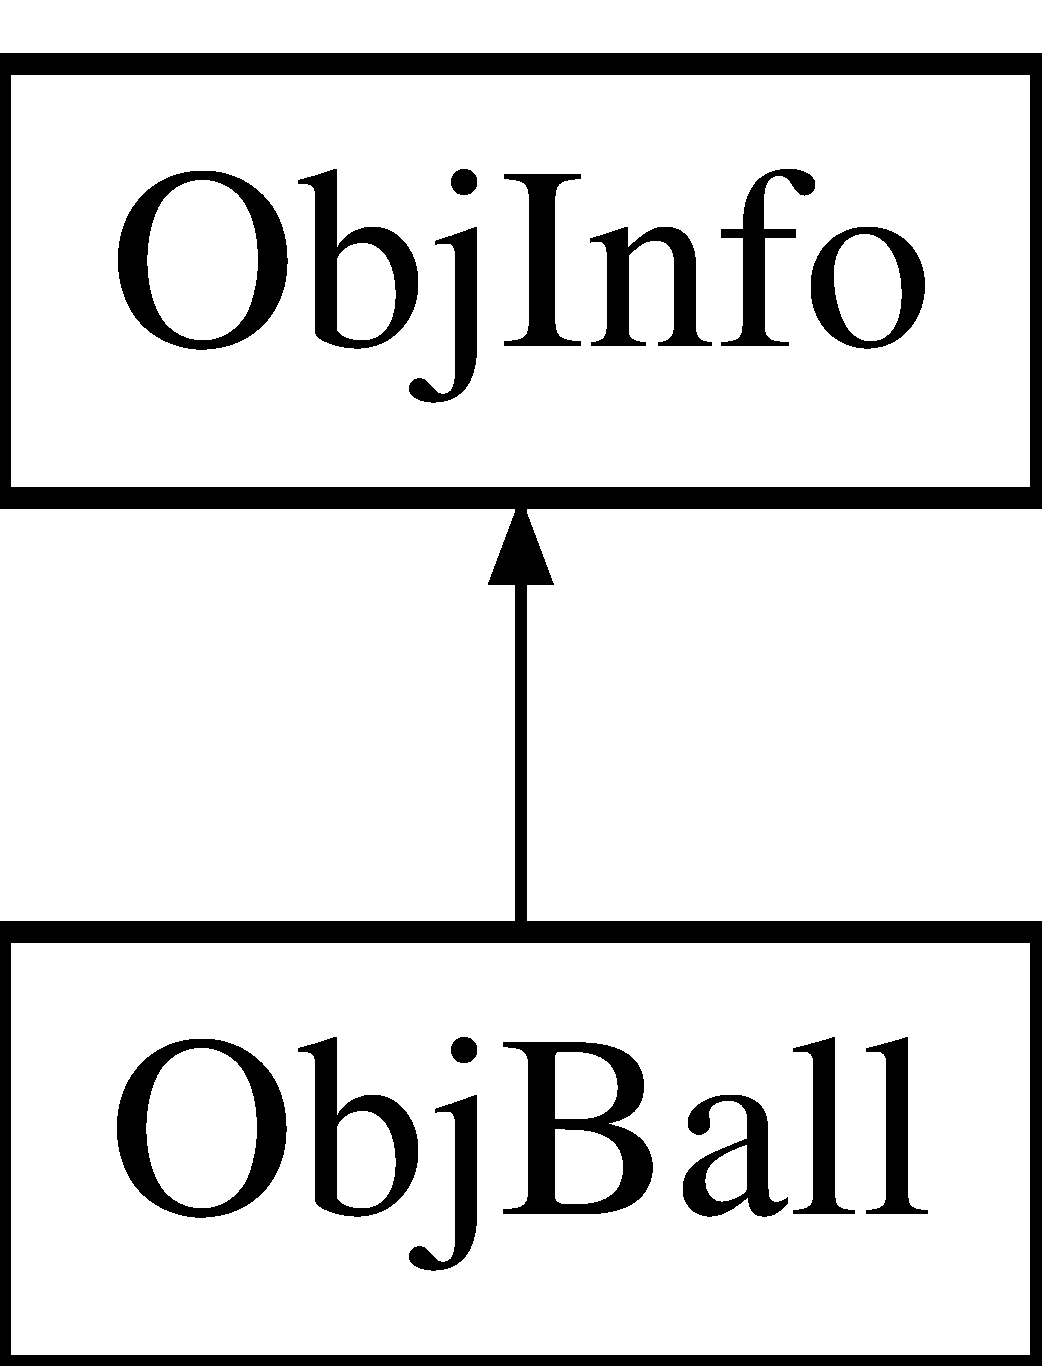
\includegraphics[height=2.000000cm]{classObjBall}
\end{center}
\end{figure}


\subsection{Detailed Description}
container for the ball \hyperlink{classObjInfo}{ObjInfo},

container for the flag \hyperlink{classObjInfo}{ObjInfo}, 

The documentation for this class was generated from the following file:\begin{DoxyCompactItemize}
\item 
\hyperlink{ObjInfo_8java}{ObjInfo.java}\end{DoxyCompactItemize}

\hypertarget{classObjFlag}{
\section{ObjFlag Class Reference}
\label{classObjFlag}\index{ObjFlag@{ObjFlag}}
}
Inheritance diagram for ObjFlag:\begin{figure}[H]
\begin{center}
\leavevmode
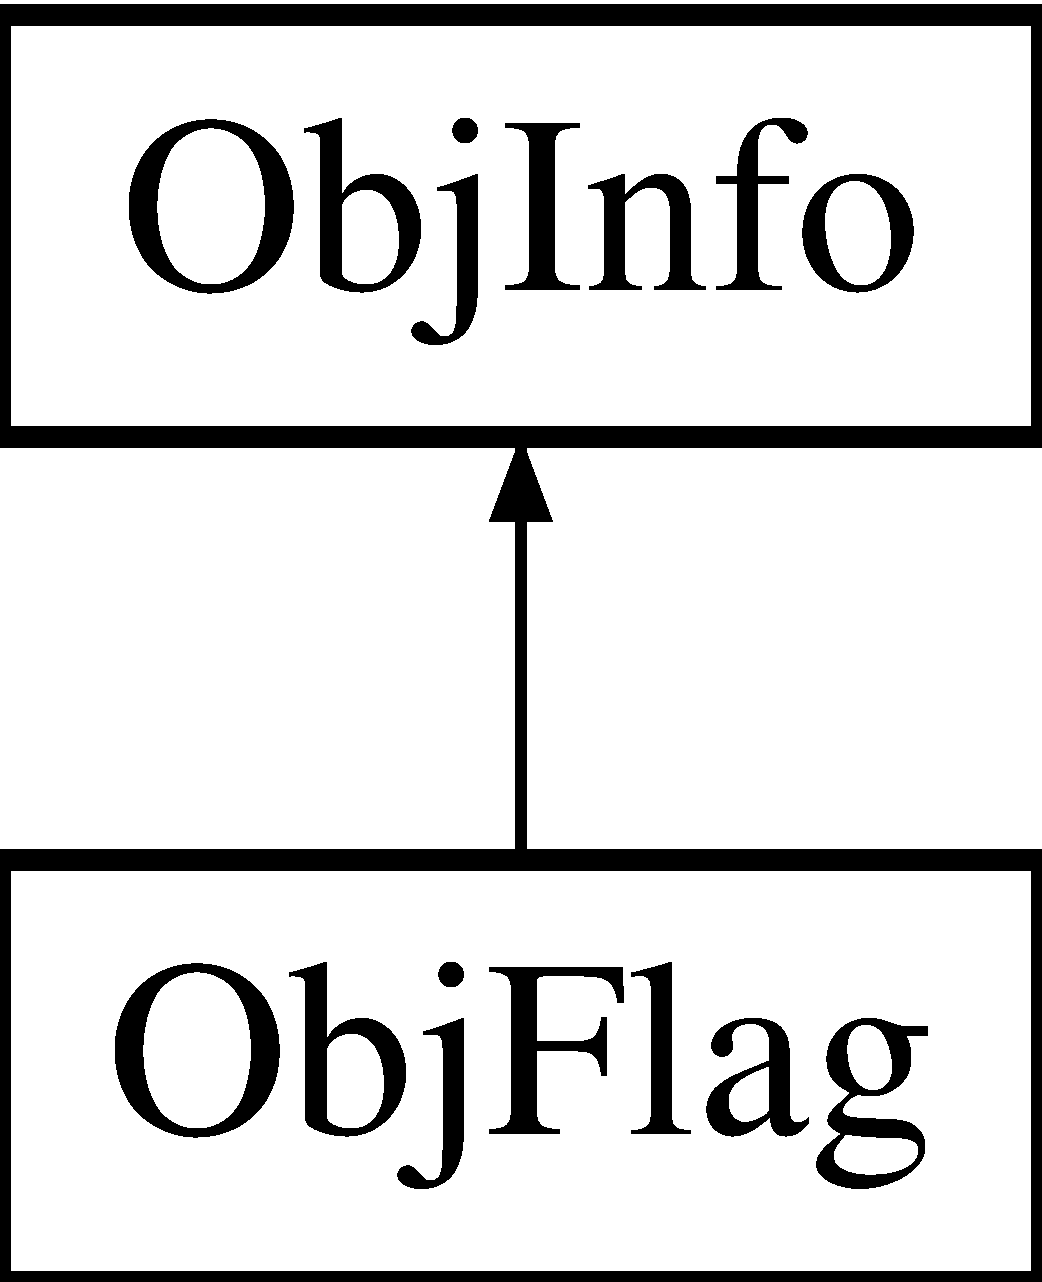
\includegraphics[height=2.000000cm]{classObjFlag}
\end{center}
\end{figure}
\subsection*{Public Member Functions}
\begin{DoxyCompactItemize}
\item 
\hyperlink{classObjFlag_a0fe2e7f04dc85a25f9975fa6e2d498e8}{ObjFlag} (String name)
\item 
String \hyperlink{classObjFlag_abafa787ef25f5a2367ae8cc37d603edb}{getFlagType} ()
\item 
void \hyperlink{classObjFlag_ae146d3a1a32eb06e0de706cb2615b736}{setFlagType} (String flagType)
\item 
String \hyperlink{classObjFlag_a05a03e912304e928e93281cbdd53c7f3}{getFlagName} ()
\item 
void \hyperlink{classObjFlag_a0cf54867f58671b491cf79a3710760c5}{setFlagName} (String name)
\item 
String \hyperlink{classObjFlag_aabcf15537dc016e0be306cf1470cee9f}{getX\_\-pos} ()
\item 
void \hyperlink{classObjFlag_aa9f908a777bc2f8a08adff6d2b622c1e}{setX\_\-pos} (String x\_\-pos)
\item 
String \hyperlink{classObjFlag_ab49184dc2174d2885dedd7e67524e69b}{getY\_\-pos} ()
\item 
void \hyperlink{classObjFlag_af1de8db60b153f2094d0a8dfd4b5d556}{setY\_\-pos} (String y\_\-pos)
\item 
String \hyperlink{classObjFlag_a5e4953a0645da52e419791223a3f44ef}{getYard} ()
\item 
void \hyperlink{classObjFlag_a8632cc6f057c18f45926eab53ca1dc48}{setYard} (String yard)
\end{DoxyCompactItemize}


\subsection{Constructor \& Destructor Documentation}
\hypertarget{classObjFlag_a0fe2e7f04dc85a25f9975fa6e2d498e8}{
\index{ObjFlag@{ObjFlag}!ObjFlag@{ObjFlag}}
\index{ObjFlag@{ObjFlag}!ObjFlag@{ObjFlag}}
\subsubsection[{ObjFlag}]{\setlength{\rightskip}{0pt plus 5cm}ObjFlag::ObjFlag (
\begin{DoxyParamCaption}
\item[{String}]{name}
\end{DoxyParamCaption}
)\hspace{0.3cm}{\ttfamily  \mbox{[}inline\mbox{]}}}}
\label{classObjFlag_a0fe2e7f04dc85a25f9975fa6e2d498e8}
Constructor of flag with flag name 

\subsection{Member Function Documentation}
\hypertarget{classObjFlag_a05a03e912304e928e93281cbdd53c7f3}{
\index{ObjFlag@{ObjFlag}!getFlagName@{getFlagName}}
\index{getFlagName@{getFlagName}!ObjFlag@{ObjFlag}}
\subsubsection[{getFlagName}]{\setlength{\rightskip}{0pt plus 5cm}String ObjFlag::getFlagName (
\begin{DoxyParamCaption}
{}
\end{DoxyParamCaption}
)\hspace{0.3cm}{\ttfamily  \mbox{[}inline\mbox{]}}}}
\label{classObjFlag_a05a03e912304e928e93281cbdd53c7f3}
The Flag Name getter

\begin{DoxyReturn}{Returns}
The name of the flag, as given by the server but with no spaces (e.g. flt20 for boundary flag left, top, 20 yard line) 
\end{DoxyReturn}
\hypertarget{classObjFlag_abafa787ef25f5a2367ae8cc37d603edb}{
\index{ObjFlag@{ObjFlag}!getFlagType@{getFlagType}}
\index{getFlagType@{getFlagType}!ObjFlag@{ObjFlag}}
\subsubsection[{getFlagType}]{\setlength{\rightskip}{0pt plus 5cm}String ObjFlag::getFlagType (
\begin{DoxyParamCaption}
{}
\end{DoxyParamCaption}
)\hspace{0.3cm}{\ttfamily  \mbox{[}inline\mbox{]}}}}
\label{classObjFlag_abafa787ef25f5a2367ae8cc37d603edb}
The Flag Type getter

\begin{DoxyReturn}{Returns}
The type of flag depending on it's location: \char`\"{}b\char`\"{} -\/ outer boundary \char`\"{}f\char`\"{} -\/ goal post \char`\"{}p\char`\"{} -\/ penalty box \char`\"{}c\char`\"{} -\/ center of field \char`\"{}l\char`\"{} -\/ border line 
\end{DoxyReturn}
\hypertarget{classObjFlag_aabcf15537dc016e0be306cf1470cee9f}{
\index{ObjFlag@{ObjFlag}!getX\_\-pos@{getX\_\-pos}}
\index{getX\_\-pos@{getX\_\-pos}!ObjFlag@{ObjFlag}}
\subsubsection[{getX\_\-pos}]{\setlength{\rightskip}{0pt plus 5cm}String ObjFlag::getX\_\-pos (
\begin{DoxyParamCaption}
{}
\end{DoxyParamCaption}
)\hspace{0.3cm}{\ttfamily  \mbox{[}inline\mbox{]}}}}
\label{classObjFlag_aabcf15537dc016e0be306cf1470cee9f}
The X position getter

\begin{DoxyReturn}{Returns}
Either \char`\"{}l\char`\"{} for left, \char`\"{}r\char`\"{} for right, or \char`\"{}c\char`\"{} for center 
\end{DoxyReturn}
\hypertarget{classObjFlag_ab49184dc2174d2885dedd7e67524e69b}{
\index{ObjFlag@{ObjFlag}!getY\_\-pos@{getY\_\-pos}}
\index{getY\_\-pos@{getY\_\-pos}!ObjFlag@{ObjFlag}}
\subsubsection[{getY\_\-pos}]{\setlength{\rightskip}{0pt plus 5cm}String ObjFlag::getY\_\-pos (
\begin{DoxyParamCaption}
{}
\end{DoxyParamCaption}
)\hspace{0.3cm}{\ttfamily  \mbox{[}inline\mbox{]}}}}
\label{classObjFlag_ab49184dc2174d2885dedd7e67524e69b}
The Y position getter

\begin{DoxyReturn}{Returns}
Either \char`\"{}t\char`\"{} for top, \char`\"{}b\char`\"{} for bottom, or \char`\"{}c\char`\"{} for center 
\end{DoxyReturn}
\hypertarget{classObjFlag_a5e4953a0645da52e419791223a3f44ef}{
\index{ObjFlag@{ObjFlag}!getYard@{getYard}}
\index{getYard@{getYard}!ObjFlag@{ObjFlag}}
\subsubsection[{getYard}]{\setlength{\rightskip}{0pt plus 5cm}String ObjFlag::getYard (
\begin{DoxyParamCaption}
{}
\end{DoxyParamCaption}
)\hspace{0.3cm}{\ttfamily  \mbox{[}inline\mbox{]}}}}
\label{classObjFlag_a5e4953a0645da52e419791223a3f44ef}
The yard getter

\begin{DoxyReturn}{Returns}
the yard is a String of a number for boundaries 
\end{DoxyReturn}
\hypertarget{classObjFlag_a0cf54867f58671b491cf79a3710760c5}{
\index{ObjFlag@{ObjFlag}!setFlagName@{setFlagName}}
\index{setFlagName@{setFlagName}!ObjFlag@{ObjFlag}}
\subsubsection[{setFlagName}]{\setlength{\rightskip}{0pt plus 5cm}void ObjFlag::setFlagName (
\begin{DoxyParamCaption}
\item[{String}]{name}
\end{DoxyParamCaption}
)\hspace{0.3cm}{\ttfamily  \mbox{[}inline\mbox{]}}}}
\label{classObjFlag_a0cf54867f58671b491cf79a3710760c5}
The Flag Name setter \hypertarget{classObjFlag_ae146d3a1a32eb06e0de706cb2615b736}{
\index{ObjFlag@{ObjFlag}!setFlagType@{setFlagType}}
\index{setFlagType@{setFlagType}!ObjFlag@{ObjFlag}}
\subsubsection[{setFlagType}]{\setlength{\rightskip}{0pt plus 5cm}void ObjFlag::setFlagType (
\begin{DoxyParamCaption}
\item[{String}]{flagType}
\end{DoxyParamCaption}
)\hspace{0.3cm}{\ttfamily  \mbox{[}inline\mbox{]}}}}
\label{classObjFlag_ae146d3a1a32eb06e0de706cb2615b736}
The Flag Type setter \hypertarget{classObjFlag_aa9f908a777bc2f8a08adff6d2b622c1e}{
\index{ObjFlag@{ObjFlag}!setX\_\-pos@{setX\_\-pos}}
\index{setX\_\-pos@{setX\_\-pos}!ObjFlag@{ObjFlag}}
\subsubsection[{setX\_\-pos}]{\setlength{\rightskip}{0pt plus 5cm}void ObjFlag::setX\_\-pos (
\begin{DoxyParamCaption}
\item[{String}]{x\_\-pos}
\end{DoxyParamCaption}
)\hspace{0.3cm}{\ttfamily  \mbox{[}inline\mbox{]}}}}
\label{classObjFlag_aa9f908a777bc2f8a08adff6d2b622c1e}
The X position setter \hypertarget{classObjFlag_af1de8db60b153f2094d0a8dfd4b5d556}{
\index{ObjFlag@{ObjFlag}!setY\_\-pos@{setY\_\-pos}}
\index{setY\_\-pos@{setY\_\-pos}!ObjFlag@{ObjFlag}}
\subsubsection[{setY\_\-pos}]{\setlength{\rightskip}{0pt plus 5cm}void ObjFlag::setY\_\-pos (
\begin{DoxyParamCaption}
\item[{String}]{y\_\-pos}
\end{DoxyParamCaption}
)\hspace{0.3cm}{\ttfamily  \mbox{[}inline\mbox{]}}}}
\label{classObjFlag_af1de8db60b153f2094d0a8dfd4b5d556}
The Y position setter \hypertarget{classObjFlag_a8632cc6f057c18f45926eab53ca1dc48}{
\index{ObjFlag@{ObjFlag}!setYard@{setYard}}
\index{setYard@{setYard}!ObjFlag@{ObjFlag}}
\subsubsection[{setYard}]{\setlength{\rightskip}{0pt plus 5cm}void ObjFlag::setYard (
\begin{DoxyParamCaption}
\item[{String}]{yard}
\end{DoxyParamCaption}
)\hspace{0.3cm}{\ttfamily  \mbox{[}inline\mbox{]}}}}
\label{classObjFlag_a8632cc6f057c18f45926eab53ca1dc48}
The yard setter 

The documentation for this class was generated from the following file:\begin{DoxyCompactItemize}
\item 
\hyperlink{ObjInfo_8java}{ObjInfo.java}\end{DoxyCompactItemize}

\hypertarget{classObjGoal}{
\section{ObjGoal Class Reference}
\label{classObjGoal}\index{ObjGoal@{ObjGoal}}
}
Inheritance diagram for ObjGoal:\begin{figure}[H]
\begin{center}
\leavevmode
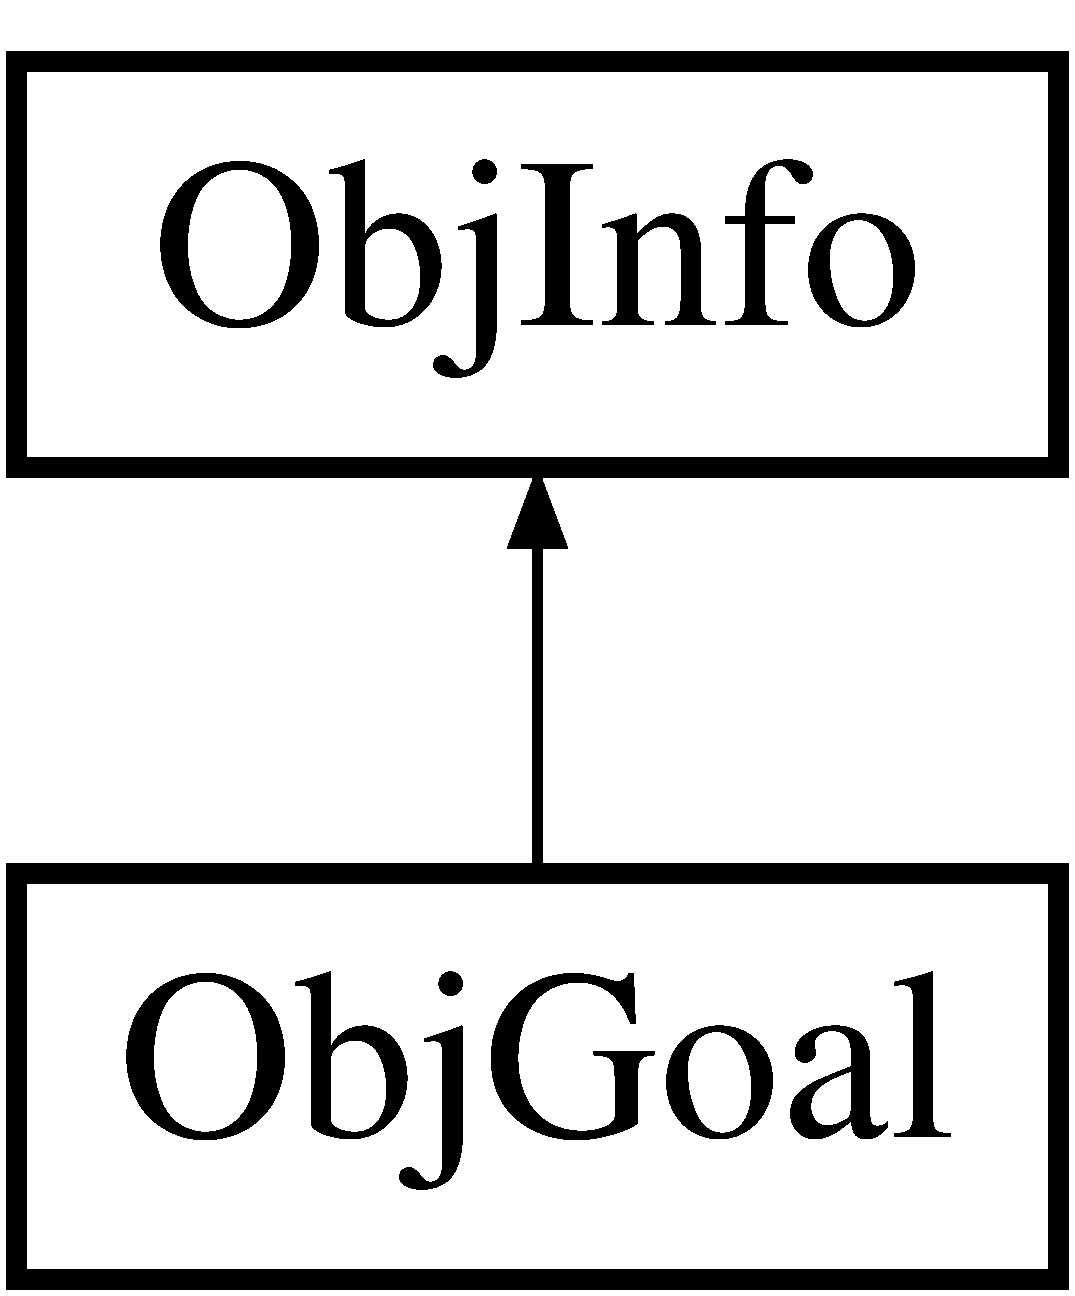
\includegraphics[height=2.000000cm]{classObjGoal}
\end{center}
\end{figure}


\subsection{Detailed Description}
container for the goal \hyperlink{classObjInfo}{ObjInfo}, 

The documentation for this class was generated from the following file:\begin{DoxyCompactItemize}
\item 
\hyperlink{ObjInfo_8java}{ObjInfo.java}\end{DoxyCompactItemize}

\hypertarget{classObjInfo}{
\section{ObjInfo Class Reference}
\label{classObjInfo}\index{ObjInfo@{ObjInfo}}
}
Inheritance diagram for ObjInfo:\begin{figure}[H]
\begin{center}
\leavevmode
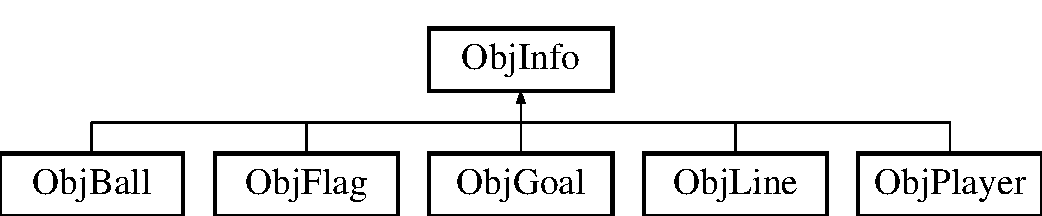
\includegraphics[height=2.000000cm]{classObjInfo}
\end{center}
\end{figure}
\subsection*{Public Member Functions}
\begin{DoxyCompactItemize}
\item 
\hyperlink{classObjInfo_ad19b0055d176cde79b5378ccdc38df3a}{ObjInfo} ()
\item 
\hyperlink{classObjInfo_a142d8b8895338edfac87db81969476f9}{ObjInfo} (String name)
\item 
String \hyperlink{classObjInfo_ad44bdb3cd59a74e08070965324ac3683}{getObjName} ()
\item 
void \hyperlink{classObjInfo_af32b13fc26020d60369b17eb6b9a9965}{setObjName} (String name)
\item 
String \hyperlink{classObjInfo_a48ed0db963d2462969cd33af9dd28118}{getSide} ()
\item 
void \hyperlink{classObjInfo_a735e078adee364209387ce08416b705a}{setSide} (String objSide)
\item 
double \hyperlink{classObjInfo_a0d4c92ca74fba99b3e7f2640229eb2d1}{getDistance} ()
\item 
void \hyperlink{classObjInfo_a378cc32e9007aaf1c9ab692e126151bc}{setDistance} (double distance)
\item 
double \hyperlink{classObjInfo_acbe5646380c4bcd20ec6a8a23f515266}{getDirection} ()
\item 
void \hyperlink{classObjInfo_af032096b1e9b5c9ca2816d9f4ac0bdbb}{setDirection} (double direction)
\item 
double \hyperlink{classObjInfo_aaee814bd674ebe17d3889d356c5a1e69}{getDistChng} ()
\item 
void \hyperlink{classObjInfo_ad0571c0aa6bd8f5703ce030a250ea98c}{setDistChng} (double distChng)
\item 
double \hyperlink{classObjInfo_a015ed333d19893a3c81776f50eb17416}{getDirChng} ()
\item 
void \hyperlink{classObjInfo_ac562af4e289c8c552ee8c471f4b43094}{setDirChng} (double dirChng)
\end{DoxyCompactItemize}


\subsection{Detailed Description}
A container for items in the Player's vision 

\subsection{Constructor \& Destructor Documentation}
\hypertarget{classObjInfo_ad19b0055d176cde79b5378ccdc38df3a}{
\index{ObjInfo@{ObjInfo}!ObjInfo@{ObjInfo}}
\index{ObjInfo@{ObjInfo}!ObjInfo@{ObjInfo}}
\subsubsection[{ObjInfo}]{\setlength{\rightskip}{0pt plus 5cm}ObjInfo::ObjInfo (
\begin{DoxyParamCaption}
{}
\end{DoxyParamCaption}
)\hspace{0.3cm}{\ttfamily  \mbox{[}inline\mbox{]}}}}
\label{classObjInfo_ad19b0055d176cde79b5378ccdc38df3a}
The Default constructor \hypertarget{classObjInfo_a142d8b8895338edfac87db81969476f9}{
\index{ObjInfo@{ObjInfo}!ObjInfo@{ObjInfo}}
\index{ObjInfo@{ObjInfo}!ObjInfo@{ObjInfo}}
\subsubsection[{ObjInfo}]{\setlength{\rightskip}{0pt plus 5cm}ObjInfo::ObjInfo (
\begin{DoxyParamCaption}
\item[{String}]{name}
\end{DoxyParamCaption}
)\hspace{0.3cm}{\ttfamily  \mbox{[}inline\mbox{]}}}}
\label{classObjInfo_a142d8b8895338edfac87db81969476f9}
The \hyperlink{classObjInfo}{ObjInfo} constructor

This initializes all the variables to 0.0 and sets the name


\begin{DoxyParams}{Parameters}
{\em name} & The type of \hyperlink{classObjInfo}{ObjInfo}, either ball, player, goal, line, or flag \\
\hline
\end{DoxyParams}


\subsection{Member Function Documentation}
\hypertarget{classObjInfo_a015ed333d19893a3c81776f50eb17416}{
\index{ObjInfo@{ObjInfo}!getDirChng@{getDirChng}}
\index{getDirChng@{getDirChng}!ObjInfo@{ObjInfo}}
\subsubsection[{getDirChng}]{\setlength{\rightskip}{0pt plus 5cm}double ObjInfo::getDirChng (
\begin{DoxyParamCaption}
{}
\end{DoxyParamCaption}
)\hspace{0.3cm}{\ttfamily  \mbox{[}inline\mbox{]}}}}
\label{classObjInfo_a015ed333d19893a3c81776f50eb17416}
The direction change getter

\begin{DoxyReturn}{Returns}
the approximate direction change (direction of velocity) of \hyperlink{classObjInfo}{ObjInfo} 
\end{DoxyReturn}
\hypertarget{classObjInfo_acbe5646380c4bcd20ec6a8a23f515266}{
\index{ObjInfo@{ObjInfo}!getDirection@{getDirection}}
\index{getDirection@{getDirection}!ObjInfo@{ObjInfo}}
\subsubsection[{getDirection}]{\setlength{\rightskip}{0pt plus 5cm}double ObjInfo::getDirection (
\begin{DoxyParamCaption}
{}
\end{DoxyParamCaption}
)\hspace{0.3cm}{\ttfamily  \mbox{[}inline\mbox{]}}}}
\label{classObjInfo_acbe5646380c4bcd20ec6a8a23f515266}
The direction getter

\begin{DoxyReturn}{Returns}
the approximate direction of \hyperlink{classObjInfo}{ObjInfo} 
\end{DoxyReturn}
\hypertarget{classObjInfo_a0d4c92ca74fba99b3e7f2640229eb2d1}{
\index{ObjInfo@{ObjInfo}!getDistance@{getDistance}}
\index{getDistance@{getDistance}!ObjInfo@{ObjInfo}}
\subsubsection[{getDistance}]{\setlength{\rightskip}{0pt plus 5cm}double ObjInfo::getDistance (
\begin{DoxyParamCaption}
{}
\end{DoxyParamCaption}
)\hspace{0.3cm}{\ttfamily  \mbox{[}inline\mbox{]}}}}
\label{classObjInfo_a0d4c92ca74fba99b3e7f2640229eb2d1}
The distance getter

\begin{DoxyReturn}{Returns}
the approximate distance to the object 
\end{DoxyReturn}
\hypertarget{classObjInfo_aaee814bd674ebe17d3889d356c5a1e69}{
\index{ObjInfo@{ObjInfo}!getDistChng@{getDistChng}}
\index{getDistChng@{getDistChng}!ObjInfo@{ObjInfo}}
\subsubsection[{getDistChng}]{\setlength{\rightskip}{0pt plus 5cm}double ObjInfo::getDistChng (
\begin{DoxyParamCaption}
{}
\end{DoxyParamCaption}
)\hspace{0.3cm}{\ttfamily  \mbox{[}inline\mbox{]}}}}
\label{classObjInfo_aaee814bd674ebe17d3889d356c5a1e69}
The distance change getter

\begin{DoxyReturn}{Returns}
the approximate distance change (magnitude of velocity) of \hyperlink{classObjInfo}{ObjInfo} 
\end{DoxyReturn}
\hypertarget{classObjInfo_ad44bdb3cd59a74e08070965324ac3683}{
\index{ObjInfo@{ObjInfo}!getObjName@{getObjName}}
\index{getObjName@{getObjName}!ObjInfo@{ObjInfo}}
\subsubsection[{getObjName}]{\setlength{\rightskip}{0pt plus 5cm}String ObjInfo::getObjName (
\begin{DoxyParamCaption}
{}
\end{DoxyParamCaption}
)\hspace{0.3cm}{\ttfamily  \mbox{[}inline\mbox{]}}}}
\label{classObjInfo_ad44bdb3cd59a74e08070965324ac3683}
The ObjName getter \hypertarget{classObjInfo_a48ed0db963d2462969cd33af9dd28118}{
\index{ObjInfo@{ObjInfo}!getSide@{getSide}}
\index{getSide@{getSide}!ObjInfo@{ObjInfo}}
\subsubsection[{getSide}]{\setlength{\rightskip}{0pt plus 5cm}String ObjInfo::getSide (
\begin{DoxyParamCaption}
{}
\end{DoxyParamCaption}
)\hspace{0.3cm}{\ttfamily  \mbox{[}inline\mbox{]}}}}
\label{classObjInfo_a48ed0db963d2462969cd33af9dd28118}
The side getter \hypertarget{classObjInfo_ac562af4e289c8c552ee8c471f4b43094}{
\index{ObjInfo@{ObjInfo}!setDirChng@{setDirChng}}
\index{setDirChng@{setDirChng}!ObjInfo@{ObjInfo}}
\subsubsection[{setDirChng}]{\setlength{\rightskip}{0pt plus 5cm}void ObjInfo::setDirChng (
\begin{DoxyParamCaption}
\item[{double}]{dirChng}
\end{DoxyParamCaption}
)\hspace{0.3cm}{\ttfamily  \mbox{[}inline\mbox{]}}}}
\label{classObjInfo_ac562af4e289c8c552ee8c471f4b43094}
The distance change setter \hypertarget{classObjInfo_af032096b1e9b5c9ca2816d9f4ac0bdbb}{
\index{ObjInfo@{ObjInfo}!setDirection@{setDirection}}
\index{setDirection@{setDirection}!ObjInfo@{ObjInfo}}
\subsubsection[{setDirection}]{\setlength{\rightskip}{0pt plus 5cm}void ObjInfo::setDirection (
\begin{DoxyParamCaption}
\item[{double}]{direction}
\end{DoxyParamCaption}
)\hspace{0.3cm}{\ttfamily  \mbox{[}inline\mbox{]}}}}
\label{classObjInfo_af032096b1e9b5c9ca2816d9f4ac0bdbb}
The direction setter \hypertarget{classObjInfo_a378cc32e9007aaf1c9ab692e126151bc}{
\index{ObjInfo@{ObjInfo}!setDistance@{setDistance}}
\index{setDistance@{setDistance}!ObjInfo@{ObjInfo}}
\subsubsection[{setDistance}]{\setlength{\rightskip}{0pt plus 5cm}void ObjInfo::setDistance (
\begin{DoxyParamCaption}
\item[{double}]{distance}
\end{DoxyParamCaption}
)\hspace{0.3cm}{\ttfamily  \mbox{[}inline\mbox{]}}}}
\label{classObjInfo_a378cc32e9007aaf1c9ab692e126151bc}
The distance setter \hypertarget{classObjInfo_ad0571c0aa6bd8f5703ce030a250ea98c}{
\index{ObjInfo@{ObjInfo}!setDistChng@{setDistChng}}
\index{setDistChng@{setDistChng}!ObjInfo@{ObjInfo}}
\subsubsection[{setDistChng}]{\setlength{\rightskip}{0pt plus 5cm}void ObjInfo::setDistChng (
\begin{DoxyParamCaption}
\item[{double}]{distChng}
\end{DoxyParamCaption}
)\hspace{0.3cm}{\ttfamily  \mbox{[}inline\mbox{]}}}}
\label{classObjInfo_ad0571c0aa6bd8f5703ce030a250ea98c}
The distance change setter \hypertarget{classObjInfo_af32b13fc26020d60369b17eb6b9a9965}{
\index{ObjInfo@{ObjInfo}!setObjName@{setObjName}}
\index{setObjName@{setObjName}!ObjInfo@{ObjInfo}}
\subsubsection[{setObjName}]{\setlength{\rightskip}{0pt plus 5cm}void ObjInfo::setObjName (
\begin{DoxyParamCaption}
\item[{String}]{name}
\end{DoxyParamCaption}
)\hspace{0.3cm}{\ttfamily  \mbox{[}inline\mbox{]}}}}
\label{classObjInfo_af32b13fc26020d60369b17eb6b9a9965}
The ObjName setter \hypertarget{classObjInfo_a735e078adee364209387ce08416b705a}{
\index{ObjInfo@{ObjInfo}!setSide@{setSide}}
\index{setSide@{setSide}!ObjInfo@{ObjInfo}}
\subsubsection[{setSide}]{\setlength{\rightskip}{0pt plus 5cm}void ObjInfo::setSide (
\begin{DoxyParamCaption}
\item[{String}]{objSide}
\end{DoxyParamCaption}
)\hspace{0.3cm}{\ttfamily  \mbox{[}inline\mbox{]}}}}
\label{classObjInfo_a735e078adee364209387ce08416b705a}
The side setter 

The documentation for this class was generated from the following file:\begin{DoxyCompactItemize}
\item 
\hyperlink{ObjInfo_8java}{ObjInfo.java}\end{DoxyCompactItemize}

\hypertarget{classObjLine}{
\section{ObjLine Class Reference}
\label{classObjLine}\index{ObjLine@{ObjLine}}
}
Inheritance diagram for ObjLine:\begin{figure}[H]
\begin{center}
\leavevmode
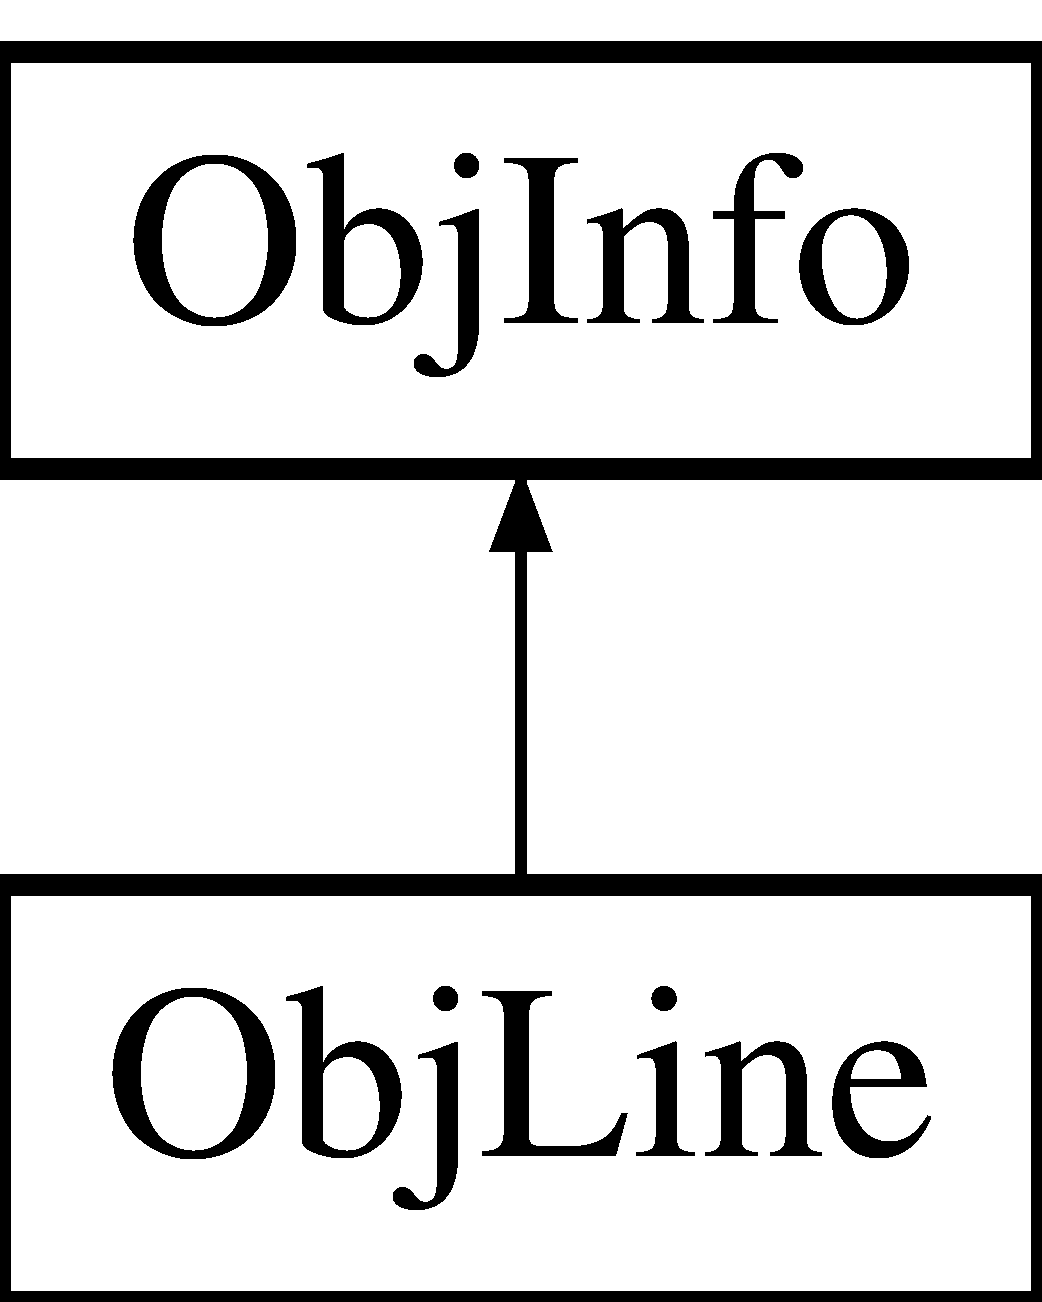
\includegraphics[height=2.000000cm]{classObjLine}
\end{center}
\end{figure}


\subsection{Detailed Description}
container for line \hyperlink{classObjInfo}{ObjInfo} 

The documentation for this class was generated from the following file:\begin{DoxyCompactItemize}
\item 
\hyperlink{ObjInfo_8java}{ObjInfo.java}\end{DoxyCompactItemize}

\hypertarget{classObjMemory}{
\section{ObjMemory Class Reference}
\label{classObjMemory}\index{ObjMemory@{ObjMemory}}
}
\subsection*{Public Member Functions}
\begin{DoxyCompactItemize}
\item 
\hyperlink{classObjMemory_a0536b9096b54697218eecf2f1da3c1b4}{ObjMemory} ()
\item 
\hyperlink{classObjMemory_a1868167dda44f86ec490e9e06cfd7bca}{ObjMemory} (ArrayList$<$ \hyperlink{classObjInfo}{ObjInfo} $>$ ObjArray, int t)
\item 
void \hyperlink{classObjMemory_a8d90e6f1f96617d419136240cac1055d}{addInfo} (\hyperlink{classObjInfo}{ObjInfo} newInfo)
\item 
int \hyperlink{classObjMemory_a6d60d4dbeb76b1acecedd12aa5aa9a7e}{getTime} ()
\item 
void \hyperlink{classObjMemory_a51b9a4241e85b64e7de03ceb23fa49c4}{setTime} (int t)
\item 
int \hyperlink{classObjMemory_aabec8724e9dcf43c1d74e07da32db6c4}{getSize} ()
\item 
\hyperlink{classObjInfo}{ObjInfo} \hyperlink{classObjMemory_a239534ad3fd257bca199db862298f701}{getObj} (int index)
\item 
\hyperlink{classObjInfo}{ObjInfo} \hyperlink{classObjMemory_ae4fb653adb8f1f399b4c5abfd824fa7a}{getObj} (String name)
\end{DoxyCompactItemize}
\subsection*{Public Attributes}
\begin{DoxyCompactItemize}
\item 
\hypertarget{classObjMemory_a7697b1cf169db1b511c22ef743c566c1}{
ArrayList$<$ \hyperlink{classObjInfo}{ObjInfo} $>$ {\bfseries ObjArray}}
\label{classObjMemory_a7697b1cf169db1b511c22ef743c566c1}

\end{DoxyCompactItemize}


\subsection{Detailed Description}
The \hyperlink{classObjMemory}{ObjMemory} saves all the \hyperlink{classObjInfo}{ObjInfo} (and it's children) objects from a parse into ArrayList along with the time parsed. 

\subsection{Constructor \& Destructor Documentation}
\hypertarget{classObjMemory_a0536b9096b54697218eecf2f1da3c1b4}{
\index{ObjMemory@{ObjMemory}!ObjMemory@{ObjMemory}}
\index{ObjMemory@{ObjMemory}!ObjMemory@{ObjMemory}}
\subsubsection[{ObjMemory}]{\setlength{\rightskip}{0pt plus 5cm}ObjMemory::ObjMemory (
\begin{DoxyParamCaption}
{}
\end{DoxyParamCaption}
)\hspace{0.3cm}{\ttfamily  \mbox{[}inline\mbox{]}}}}
\label{classObjMemory_a0536b9096b54697218eecf2f1da3c1b4}
Default constructor

This initializes the time to 0 \hypertarget{classObjMemory_a1868167dda44f86ec490e9e06cfd7bca}{
\index{ObjMemory@{ObjMemory}!ObjMemory@{ObjMemory}}
\index{ObjMemory@{ObjMemory}!ObjMemory@{ObjMemory}}
\subsubsection[{ObjMemory}]{\setlength{\rightskip}{0pt plus 5cm}ObjMemory::ObjMemory (
\begin{DoxyParamCaption}
\item[{ArrayList$<$ {\bf ObjInfo} $>$}]{ObjArray, }
\item[{int}]{t}
\end{DoxyParamCaption}
)\hspace{0.3cm}{\ttfamily  \mbox{[}inline\mbox{]}}}}
\label{classObjMemory_a1868167dda44f86ec490e9e06cfd7bca}
\hyperlink{classObjMemory}{ObjMemory} constructor


\begin{DoxyParams}{Parameters}
{\em ObjArray} & the ArrayList containing all the ObjInfos from the server's parsed (see) message \\
\hline
{\em t} & the time parsed from the server's (see) message \\
\hline
\end{DoxyParams}
\begin{DoxyPrecond}{Precondition}
This should only be called inside of the parser. It's merely a way to store ObjInfos from the (see) message into the greater \hyperlink{classMemory}{Memory} class 
\end{DoxyPrecond}
\begin{DoxyPostcond}{Postcondition}
A new \hyperlink{classObjMemory}{ObjMemory} containing the list of visible ObjInfos and the most recent time will be availbe to add to the \hyperlink{classMemory}{Memory} 
\end{DoxyPostcond}


\subsection{Member Function Documentation}
\hypertarget{classObjMemory_a8d90e6f1f96617d419136240cac1055d}{
\index{ObjMemory@{ObjMemory}!addInfo@{addInfo}}
\index{addInfo@{addInfo}!ObjMemory@{ObjMemory}}
\subsubsection[{addInfo}]{\setlength{\rightskip}{0pt plus 5cm}void ObjMemory::addInfo (
\begin{DoxyParamCaption}
\item[{{\bf ObjInfo}}]{newInfo}
\end{DoxyParamCaption}
)\hspace{0.3cm}{\ttfamily  \mbox{[}inline\mbox{]}}}}
\label{classObjMemory_a8d90e6f1f96617d419136240cac1055d}
A method to add new \hyperlink{classObjInfo}{ObjInfo} to the \hyperlink{classObjMemory}{ObjMemory}


\begin{DoxyParams}{Parameters}
{\em newInfo} & the \hyperlink{classObjInfo}{ObjInfo} to add tot he ObjMemory's ArrayList \\
\hline
\end{DoxyParams}
\begin{DoxyPrecond}{Precondition}
A non-\/null \hyperlink{classObjInfo}{ObjInfo} will be passed into the method 
\end{DoxyPrecond}
\begin{DoxyPostcond}{Postcondition}
The newInfo will be added to the ObjArray 
\end{DoxyPostcond}
\hypertarget{classObjMemory_a239534ad3fd257bca199db862298f701}{
\index{ObjMemory@{ObjMemory}!getObj@{getObj}}
\index{getObj@{getObj}!ObjMemory@{ObjMemory}}
\subsubsection[{getObj}]{\setlength{\rightskip}{0pt plus 5cm}{\bf ObjInfo} ObjMemory::getObj (
\begin{DoxyParamCaption}
\item[{int}]{index}
\end{DoxyParamCaption}
)\hspace{0.3cm}{\ttfamily  \mbox{[}inline\mbox{]}}}}
\label{classObjMemory_a239534ad3fd257bca199db862298f701}
An accessor of individual \hyperlink{classObjInfo}{ObjInfo}


\begin{DoxyParams}{Parameters}
{\em index} & the index of the \hyperlink{classObjInfo}{ObjInfo} to retrieve \\
\hline
\end{DoxyParams}
\begin{DoxyPrecond}{Precondition}
The ObjArray should have at least one \hyperlink{classObjInfo}{ObjInfo} in it 
\end{DoxyPrecond}
\begin{DoxyPostcond}{Postcondition}
The \hyperlink{classObjInfo}{ObjInfo} at the given index will be returned, this is a good way to traverse the ObjInfos visible to you 
\end{DoxyPostcond}
\hypertarget{classObjMemory_ae4fb653adb8f1f399b4c5abfd824fa7a}{
\index{ObjMemory@{ObjMemory}!getObj@{getObj}}
\index{getObj@{getObj}!ObjMemory@{ObjMemory}}
\subsubsection[{getObj}]{\setlength{\rightskip}{0pt plus 5cm}{\bf ObjInfo} ObjMemory::getObj (
\begin{DoxyParamCaption}
\item[{String}]{name}
\end{DoxyParamCaption}
)\hspace{0.3cm}{\ttfamily  \mbox{[}inline\mbox{]}}}}
\label{classObjMemory_ae4fb653adb8f1f399b4c5abfd824fa7a}
A method to get an \hyperlink{classObjInfo}{ObjInfo} by name


\begin{DoxyParams}{Parameters}
{\em name} & the ObjName of the \hyperlink{classObjInfo}{ObjInfo} searched for (e.g. \char`\"{}ball\char`\"{})\\
\hline
\end{DoxyParams}
\begin{DoxyPrecond}{Precondition}
The \hyperlink{classObjInfo}{ObjInfo} should be checked for visibility first, otherwise you run the risk of getting an empty \hyperlink{classObjInfo}{ObjInfo} 
\end{DoxyPrecond}
\begin{DoxyPostcond}{Postcondition}
The first \hyperlink{classObjInfo}{ObjInfo} with the name will be returned. Remember, this won't return all the ObjInfos of an ObjName, if there are multiple. 
\end{DoxyPostcond}
\hypertarget{classObjMemory_aabec8724e9dcf43c1d74e07da32db6c4}{
\index{ObjMemory@{ObjMemory}!getSize@{getSize}}
\index{getSize@{getSize}!ObjMemory@{ObjMemory}}
\subsubsection[{getSize}]{\setlength{\rightskip}{0pt plus 5cm}int ObjMemory::getSize (
\begin{DoxyParamCaption}
{}
\end{DoxyParamCaption}
)\hspace{0.3cm}{\ttfamily  \mbox{[}inline\mbox{]}}}}
\label{classObjMemory_aabec8724e9dcf43c1d74e07da32db6c4}
Returns the size of the ObjArray \hypertarget{classObjMemory_a6d60d4dbeb76b1acecedd12aa5aa9a7e}{
\index{ObjMemory@{ObjMemory}!getTime@{getTime}}
\index{getTime@{getTime}!ObjMemory@{ObjMemory}}
\subsubsection[{getTime}]{\setlength{\rightskip}{0pt plus 5cm}int ObjMemory::getTime (
\begin{DoxyParamCaption}
{}
\end{DoxyParamCaption}
)\hspace{0.3cm}{\ttfamily  \mbox{[}inline\mbox{]}}}}
\label{classObjMemory_a6d60d4dbeb76b1acecedd12aa5aa9a7e}
A method to access the time the message was parsed, provided by the server's (see) message \hypertarget{classObjMemory_a51b9a4241e85b64e7de03ceb23fa49c4}{
\index{ObjMemory@{ObjMemory}!setTime@{setTime}}
\index{setTime@{setTime}!ObjMemory@{ObjMemory}}
\subsubsection[{setTime}]{\setlength{\rightskip}{0pt plus 5cm}void ObjMemory::setTime (
\begin{DoxyParamCaption}
\item[{int}]{t}
\end{DoxyParamCaption}
)\hspace{0.3cm}{\ttfamily  \mbox{[}inline\mbox{]}}}}
\label{classObjMemory_a51b9a4241e85b64e7de03ceb23fa49c4}
The time setter


\begin{DoxyParams}{Parameters}
{\em t} & the time integer from the server's latest (see) parse \\
\hline
\end{DoxyParams}
\begin{DoxyPostcond}{Postcondition}
the time will be set and ready to access 
\end{DoxyPostcond}


The documentation for this class was generated from the following file:\begin{DoxyCompactItemize}
\item 
\hyperlink{ObjMemory_8java}{ObjMemory.java}\end{DoxyCompactItemize}

\hypertarget{classObjPlayer}{
\section{ObjPlayer Class Reference}
\label{classObjPlayer}\index{ObjPlayer@{ObjPlayer}}
}
Inheritance diagram for ObjPlayer:\begin{figure}[H]
\begin{center}
\leavevmode
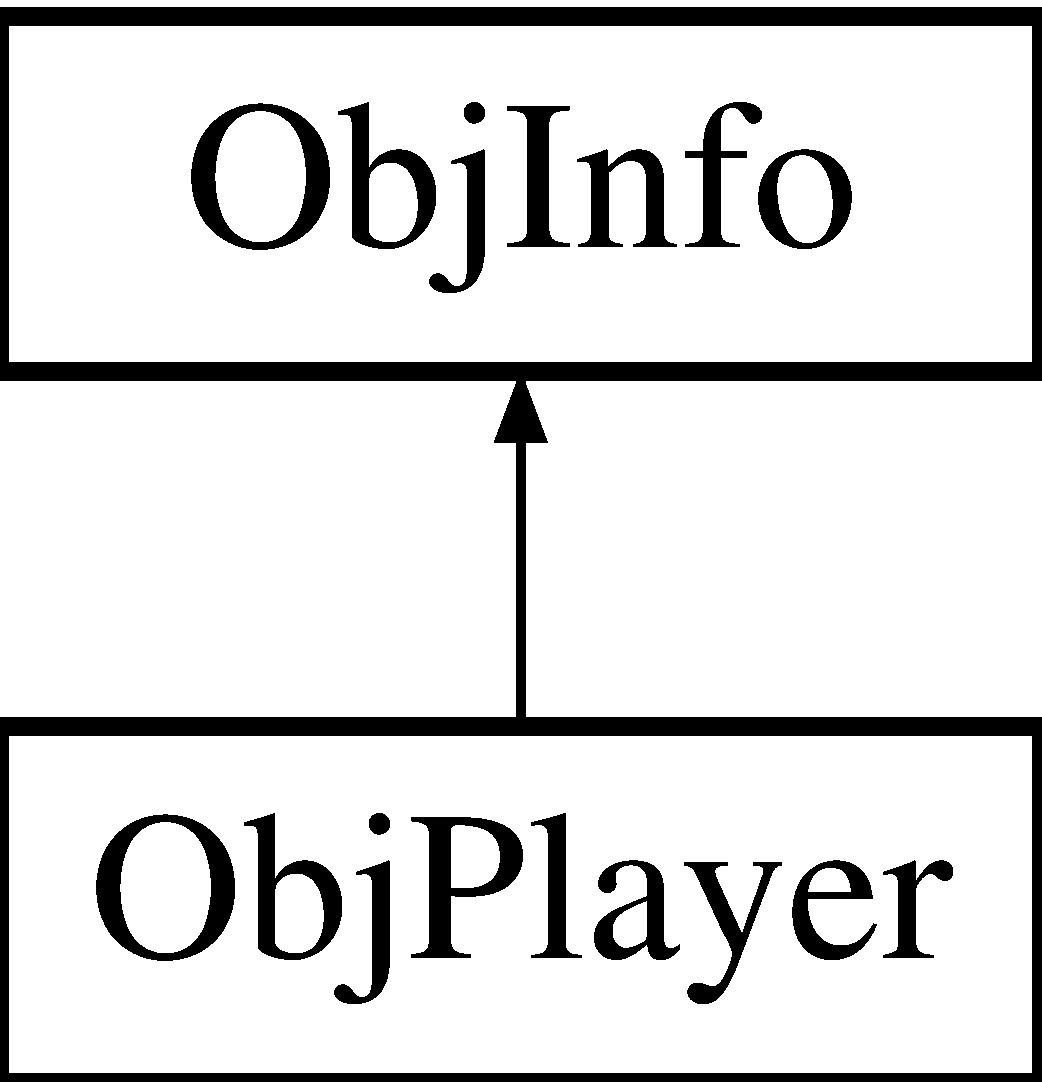
\includegraphics[height=2.000000cm]{classObjPlayer}
\end{center}
\end{figure}
\subsection*{Public Member Functions}
\begin{DoxyCompactItemize}
\item 
String \hyperlink{classObjPlayer_a52c8a9ee1da012abb60b7379e7763597}{getTeam} ()
\item 
void \hyperlink{classObjPlayer_ad1fa8b66e930eed448c800a6b80ee055}{setTeam} (String team)
\item 
int \hyperlink{classObjPlayer_a1d763181bd909af9fff3189cf014035f}{getuNum} ()
\item 
void \hyperlink{classObjPlayer_ae80af0d4c2cce1f90d0320ec2599c70e}{setuNum} (int uNum)
\item 
boolean \hyperlink{classObjPlayer_a74c9503f5232d9341a721b863c851fde}{isGoalie} ()
\item 
void \hyperlink{classObjPlayer_ad945cc86f383fed367bdda2b36a3e2ac}{setGoalie} (boolean goalie)
\item 
double \hyperlink{classObjPlayer_ad842a68637343da6ae9e5fbd361947a6}{getHeadDir} ()
\item 
void \hyperlink{classObjPlayer_a09a92949b4eb26e17ecb181f7d02001d}{setHeadDir} (double headDir)
\item 
double \hyperlink{classObjPlayer_a878c43dd285c24ab44fcb0a9b5aa3b62}{getBodyDir} ()
\item 
void \hyperlink{classObjPlayer_a002a52bb5e7b1c08e2585c335dc40023}{setBodyDir} (double bodyDir)
\end{DoxyCompactItemize}


\subsection{Detailed Description}
container for player \hyperlink{classObjInfo}{ObjInfo} 

\subsection{Member Function Documentation}
\hypertarget{classObjPlayer_a878c43dd285c24ab44fcb0a9b5aa3b62}{
\index{ObjPlayer@{ObjPlayer}!getBodyDir@{getBodyDir}}
\index{getBodyDir@{getBodyDir}!ObjPlayer@{ObjPlayer}}
\subsubsection[{getBodyDir}]{\setlength{\rightskip}{0pt plus 5cm}double ObjPlayer::getBodyDir (
\begin{DoxyParamCaption}
{}
\end{DoxyParamCaption}
)\hspace{0.3cm}{\ttfamily  \mbox{[}inline\mbox{]}}}}
\label{classObjPlayer_a878c43dd285c24ab44fcb0a9b5aa3b62}
A getter for the player's body direction

\begin{DoxyReturn}{Returns}
a double of the angle, in degrees, of the direction of the player's body relative to your own. The angle is 0 if their bodies are both facing each other. 
\end{DoxyReturn}
\hypertarget{classObjPlayer_ad842a68637343da6ae9e5fbd361947a6}{
\index{ObjPlayer@{ObjPlayer}!getHeadDir@{getHeadDir}}
\index{getHeadDir@{getHeadDir}!ObjPlayer@{ObjPlayer}}
\subsubsection[{getHeadDir}]{\setlength{\rightskip}{0pt plus 5cm}double ObjPlayer::getHeadDir (
\begin{DoxyParamCaption}
{}
\end{DoxyParamCaption}
)\hspace{0.3cm}{\ttfamily  \mbox{[}inline\mbox{]}}}}
\label{classObjPlayer_ad842a68637343da6ae9e5fbd361947a6}
A getter for the player's head direction

\begin{DoxyReturn}{Returns}
a double of the angle, in degrees, of the direction of the player's head relative to your own. The angle is 0 if they are both facing each other. 
\end{DoxyReturn}
\hypertarget{classObjPlayer_a52c8a9ee1da012abb60b7379e7763597}{
\index{ObjPlayer@{ObjPlayer}!getTeam@{getTeam}}
\index{getTeam@{getTeam}!ObjPlayer@{ObjPlayer}}
\subsubsection[{getTeam}]{\setlength{\rightskip}{0pt plus 5cm}String ObjPlayer::getTeam (
\begin{DoxyParamCaption}
{}
\end{DoxyParamCaption}
)\hspace{0.3cm}{\ttfamily  \mbox{[}inline\mbox{]}}}}
\label{classObjPlayer_a52c8a9ee1da012abb60b7379e7763597}
The Team Name getter

\begin{DoxyReturn}{Returns}
the name of the team the player is on, if they're close enough to see the team 
\end{DoxyReturn}
\hypertarget{classObjPlayer_a1d763181bd909af9fff3189cf014035f}{
\index{ObjPlayer@{ObjPlayer}!getuNum@{getuNum}}
\index{getuNum@{getuNum}!ObjPlayer@{ObjPlayer}}
\subsubsection[{getuNum}]{\setlength{\rightskip}{0pt plus 5cm}int ObjPlayer::getuNum (
\begin{DoxyParamCaption}
{}
\end{DoxyParamCaption}
)\hspace{0.3cm}{\ttfamily  \mbox{[}inline\mbox{]}}}}
\label{classObjPlayer_a1d763181bd909af9fff3189cf014035f}
The Uniform Number getter

\begin{DoxyReturn}{Returns}
the Uniform Number on the player's shirt, if they're close enough to see it 
\end{DoxyReturn}
\hypertarget{classObjPlayer_a74c9503f5232d9341a721b863c851fde}{
\index{ObjPlayer@{ObjPlayer}!isGoalie@{isGoalie}}
\index{isGoalie@{isGoalie}!ObjPlayer@{ObjPlayer}}
\subsubsection[{isGoalie}]{\setlength{\rightskip}{0pt plus 5cm}boolean ObjPlayer::isGoalie (
\begin{DoxyParamCaption}
{}
\end{DoxyParamCaption}
)\hspace{0.3cm}{\ttfamily  \mbox{[}inline\mbox{]}}}}
\label{classObjPlayer_a74c9503f5232d9341a721b863c851fde}
A check to see if the player is a goalie or field player

\begin{DoxyReturn}{Returns}
true if the player is the goalie, false if s/he is not 
\end{DoxyReturn}
\hypertarget{classObjPlayer_a002a52bb5e7b1c08e2585c335dc40023}{
\index{ObjPlayer@{ObjPlayer}!setBodyDir@{setBodyDir}}
\index{setBodyDir@{setBodyDir}!ObjPlayer@{ObjPlayer}}
\subsubsection[{setBodyDir}]{\setlength{\rightskip}{0pt plus 5cm}void ObjPlayer::setBodyDir (
\begin{DoxyParamCaption}
\item[{double}]{bodyDir}
\end{DoxyParamCaption}
)\hspace{0.3cm}{\ttfamily  \mbox{[}inline\mbox{]}}}}
\label{classObjPlayer_a002a52bb5e7b1c08e2585c335dc40023}
The body direction setter \hypertarget{classObjPlayer_ad945cc86f383fed367bdda2b36a3e2ac}{
\index{ObjPlayer@{ObjPlayer}!setGoalie@{setGoalie}}
\index{setGoalie@{setGoalie}!ObjPlayer@{ObjPlayer}}
\subsubsection[{setGoalie}]{\setlength{\rightskip}{0pt plus 5cm}void ObjPlayer::setGoalie (
\begin{DoxyParamCaption}
\item[{boolean}]{goalie}
\end{DoxyParamCaption}
)\hspace{0.3cm}{\ttfamily  \mbox{[}inline\mbox{]}}}}
\label{classObjPlayer_ad945cc86f383fed367bdda2b36a3e2ac}
The goalie check setter \hypertarget{classObjPlayer_a09a92949b4eb26e17ecb181f7d02001d}{
\index{ObjPlayer@{ObjPlayer}!setHeadDir@{setHeadDir}}
\index{setHeadDir@{setHeadDir}!ObjPlayer@{ObjPlayer}}
\subsubsection[{setHeadDir}]{\setlength{\rightskip}{0pt plus 5cm}void ObjPlayer::setHeadDir (
\begin{DoxyParamCaption}
\item[{double}]{headDir}
\end{DoxyParamCaption}
)\hspace{0.3cm}{\ttfamily  \mbox{[}inline\mbox{]}}}}
\label{classObjPlayer_a09a92949b4eb26e17ecb181f7d02001d}
The head direction setter \hypertarget{classObjPlayer_ad1fa8b66e930eed448c800a6b80ee055}{
\index{ObjPlayer@{ObjPlayer}!setTeam@{setTeam}}
\index{setTeam@{setTeam}!ObjPlayer@{ObjPlayer}}
\subsubsection[{setTeam}]{\setlength{\rightskip}{0pt plus 5cm}void ObjPlayer::setTeam (
\begin{DoxyParamCaption}
\item[{String}]{team}
\end{DoxyParamCaption}
)\hspace{0.3cm}{\ttfamily  \mbox{[}inline\mbox{]}}}}
\label{classObjPlayer_ad1fa8b66e930eed448c800a6b80ee055}
The Team Name setter \hypertarget{classObjPlayer_ae80af0d4c2cce1f90d0320ec2599c70e}{
\index{ObjPlayer@{ObjPlayer}!setuNum@{setuNum}}
\index{setuNum@{setuNum}!ObjPlayer@{ObjPlayer}}
\subsubsection[{setuNum}]{\setlength{\rightskip}{0pt plus 5cm}void ObjPlayer::setuNum (
\begin{DoxyParamCaption}
\item[{int}]{uNum}
\end{DoxyParamCaption}
)\hspace{0.3cm}{\ttfamily  \mbox{[}inline\mbox{]}}}}
\label{classObjPlayer_ae80af0d4c2cce1f90d0320ec2599c70e}
The Uniform Number getter 

The documentation for this class was generated from the following file:\begin{DoxyCompactItemize}
\item 
\hyperlink{ObjInfo_8java}{ObjInfo.java}\end{DoxyCompactItemize}

\hypertarget{classParser}{
\section{Parser Class Reference}
\label{classParser}\index{Parser@{Parser}}
}
\subsection*{Public Member Functions}
\begin{DoxyCompactItemize}
\item 
\hyperlink{classParser_a12234f6cd36b61af4b50c94a179422c1}{Parser} ()
\item 
void \hyperlink{classParser_a9fd1e7c4efe939758e068ff86dd7d0ee}{initParse} (String inputPacket, \hyperlink{classMemory}{Memory} mem)
\item 
void \hyperlink{classParser_acfa0b687be8aceb35d9e3c1a66308778}{Parse} (String inputPacket, \hyperlink{classMemory}{Memory} InfoMem)
\end{DoxyCompactItemize}
\subsection*{Public Attributes}
\begin{DoxyCompactItemize}
\item 
String \hyperlink{classParser_a7b23ca1da91ad5e2256afef7629901cd}{input}
\end{DoxyCompactItemize}


\subsection{Detailed Description}
This class takes in the the messages sent by the parser and parses them into information that can be stored in \hyperlink{classMemory}{Memory} and used by Players. 

\subsection{Constructor \& Destructor Documentation}
\hypertarget{classParser_a12234f6cd36b61af4b50c94a179422c1}{
\index{Parser@{Parser}!Parser@{Parser}}
\index{Parser@{Parser}!Parser@{Parser}}
\subsubsection[{Parser}]{\setlength{\rightskip}{0pt plus 5cm}Parser::Parser (
\begin{DoxyParamCaption}
{}
\end{DoxyParamCaption}
)\hspace{0.3cm}{\ttfamily  \mbox{[}inline\mbox{]}}}}
\label{classParser_a12234f6cd36b61af4b50c94a179422c1}
Default constructor 

\subsection{Member Function Documentation}
\hypertarget{classParser_a9fd1e7c4efe939758e068ff86dd7d0ee}{
\index{Parser@{Parser}!initParse@{initParse}}
\index{initParse@{initParse}!Parser@{Parser}}
\subsubsection[{initParse}]{\setlength{\rightskip}{0pt plus 5cm}void Parser::initParse (
\begin{DoxyParamCaption}
\item[{String}]{inputPacket, }
\item[{{\bf Memory}}]{mem}
\end{DoxyParamCaption}
)\hspace{0.3cm}{\ttfamily  \mbox{[}inline\mbox{]}}}}
\label{classParser_a9fd1e7c4efe939758e068ff86dd7d0ee}
This parses the (init) message, the first message sent by the server, directly after a new \hyperlink{classPlayer}{Player} is initialized.


\begin{DoxyParams}{Parameters}
{\em inputPacket} & The init message from the server \\
\hline
{\em mem} & the player's memory \\
\hline
\end{DoxyParams}
\begin{DoxyPrecond}{Precondition}
A memory must be created for the information to be stored in, and this must be called directly after an (init) is sent to the server. 
\end{DoxyPrecond}
\begin{DoxyPostcond}{Postcondition}
Vital information about the \hyperlink{classPlayer}{Player} will be saved, such as the side of the field the player starts on, the Player's uniform number and the play mode, which is \char`\"{}before\_\-kickoff.\char`\"{} 
\end{DoxyPostcond}
\hypertarget{classParser_acfa0b687be8aceb35d9e3c1a66308778}{
\index{Parser@{Parser}!Parse@{Parse}}
\index{Parse@{Parse}!Parser@{Parser}}
\subsubsection[{Parse}]{\setlength{\rightskip}{0pt plus 5cm}void Parser::Parse (
\begin{DoxyParamCaption}
\item[{String}]{inputPacket, }
\item[{{\bf Memory}}]{InfoMem}
\end{DoxyParamCaption}
)\hspace{0.3cm}{\ttfamily  \mbox{[}inline\mbox{]}}}}
\label{classParser_acfa0b687be8aceb35d9e3c1a66308778}
The actual message Parsing method


\begin{DoxyParams}{Parameters}
{\em inputPacket} & the incoming String message from the server \\
\hline
{\em InfoMem} & the \hyperlink{classMemory}{Memory} to store all the information in \\
\hline
\end{DoxyParams}
\begin{DoxyPrecond}{Precondition}
A \hyperlink{classMemory}{Memory} must be created and passed in, along with the message from the server 
\end{DoxyPrecond}
\begin{DoxyPostcond}{Postcondition}
The message will be parsed and stored either as SenseInfos from the (sense\_\-body) message, or ObjInfos from the (see) message, or the playMode from the referee (hear) message 
\end{DoxyPostcond}


\subsection{Member Data Documentation}
\hypertarget{classParser_a7b23ca1da91ad5e2256afef7629901cd}{
\index{Parser@{Parser}!input@{input}}
\index{input@{input}!Parser@{Parser}}
\subsubsection[{input}]{\setlength{\rightskip}{0pt plus 5cm}String {\bf Parser::input}}}
\label{classParser_a7b23ca1da91ad5e2256afef7629901cd}
The String of the incoming message 

The documentation for this class was generated from the following file:\begin{DoxyCompactItemize}
\item 
\hyperlink{Parser_8java}{Parser.java}\end{DoxyCompactItemize}

\hypertarget{classPlayer}{
\section{Player Class Reference}
\label{classPlayer}\index{Player@{Player}}
}
Inheritance diagram for Player:\begin{figure}[H]
\begin{center}
\leavevmode
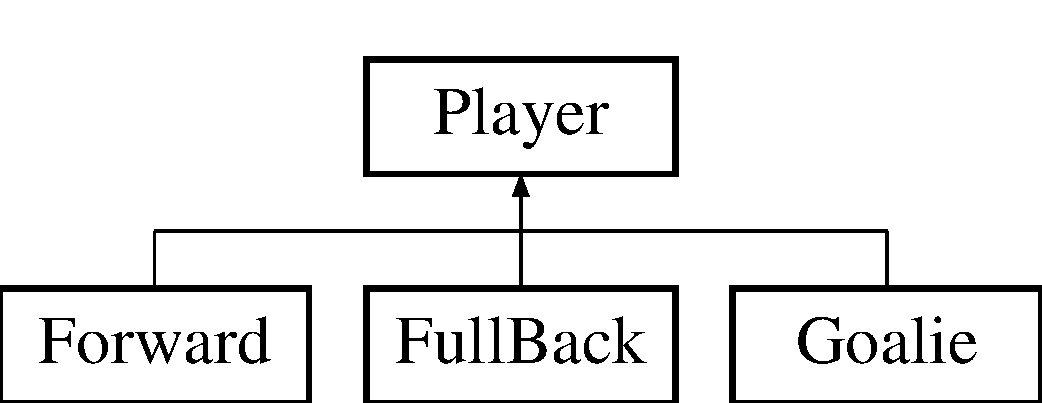
\includegraphics[height=2.000000cm]{classPlayer}
\end{center}
\end{figure}
\subsection*{Public Member Functions}
\begin{DoxyCompactItemize}
\item 
\hypertarget{classPlayer_a072996becca020ca2c95b241eee356e3}{
{\bfseries Player} (String team)}
\label{classPlayer_a072996becca020ca2c95b241eee356e3}

\item 
\hyperlink{classPlayer_afe31dd3fe679bcba10385271c37ffd1a}{Player} (\hyperlink{classRoboClient}{RoboClient} rc, \hyperlink{classMemory}{Memory} m, \hyperlink{classObjInfo}{ObjInfo} i, \hyperlink{classParser}{Parser} p, int time)
\item 
\hypertarget{classPlayer_aaec2cce8cabaa09250aa111b5a189877}{
\hyperlink{classAction}{Action} {\bfseries getAction} ()}
\label{classPlayer_aaec2cce8cabaa09250aa111b5a189877}

\item 
\hypertarget{classPlayer_ae3515d6fa2bc0f9a5b1f3c754d9010f9}{
void {\bfseries setAction} (\hyperlink{classAction}{Action} a)}
\label{classPlayer_ae3515d6fa2bc0f9a5b1f3c754d9010f9}

\item 
\hypertarget{classPlayer_a37c708420f7230019e80d664533eddc8}{
void {\bfseries setHome} (\hyperlink{classPos}{Pos} home)}
\label{classPlayer_a37c708420f7230019e80d664533eddc8}

\item 
\hypertarget{classPlayer_a90a227e48446e51923377c495b39f008}{
\hyperlink{classPos}{Pos} {\bfseries getHome} ()}
\label{classPlayer_a90a227e48446e51923377c495b39f008}

\item 
\hyperlink{classRoboClient}{RoboClient} \hyperlink{classPlayer_a633389a933930a00f75601ea957caa83}{getRoboClient} ()
\item 
void \hyperlink{classPlayer_a70a35e4a1de2cc70d947adffc0e2d580}{setRoboclient} (\hyperlink{classRoboClient}{RoboClient} rc)
\item 
\hyperlink{classMemory}{Memory} \hyperlink{classPlayer_ab43d9af06168c486d9fa0539103102a0}{getMem} ()
\item 
void \hyperlink{classPlayer_a92bd7c2bbebfc30ec332d6e6b182f9a8}{setMem} (\hyperlink{classMemory}{Memory} m)
\item 
\hyperlink{classObjInfo}{ObjInfo} \hyperlink{classPlayer_a6ca7539da0375519ff9f5993b19073f0}{getObjInfo} ()
\item 
void \hyperlink{classPlayer_a51bf665263845828767153fb4b418337}{setObjInfo} (\hyperlink{classObjInfo}{ObjInfo} i)
\item 
\hyperlink{classParser}{Parser} \hyperlink{classPlayer_a8898fbd58b68f21318bd83a3a4446a1f}{getParser} ()
\item 
void \hyperlink{classPlayer_a914ba43cef17a1ce6f210311155925a6}{setParser} (\hyperlink{classParser}{Parser} p)
\item 
\hypertarget{classPlayer_a0f037644cf072cb8f24cd98919be4a02}{
int {\bfseries getMemTime} ()}
\label{classPlayer_a0f037644cf072cb8f24cd98919be4a02}

\item 
int \hyperlink{classPlayer_a0405759b5c1c513a387b09739c271743}{getTime} ()
\item 
void \hyperlink{classPlayer_afca6d7498e56e2e82ddea7e89395a146}{setTime} (int time)
\item 
double \hyperlink{classPlayer_a2ff5bd2585d3d7388dce85576002c668}{getDirection} ()
\item 
\hyperlink{classPos}{Pos} \hyperlink{classPlayer_ae1947ff6dfb298de4699f9f79ea221cf}{getPosition} ()
\item 
void \hyperlink{classPlayer_aa826be330bb3dc6bf7bb8ac04250fe50}{initPlayer} (double x, double y, String pos)  throws SocketException, UnknownHostException 
\item 
void \hyperlink{classPlayer_a29c711f9c1d5bb762611f8e0f8c2fd47}{initPlayer} (double x, double y)  throws SocketException, UnknownHostException 
\item 
void \hyperlink{classPlayer_a65f067086737b201d4183a1bb258e7ac}{receiveInput} ()  throws InterruptedException  
\item 
void \hyperlink{classPlayer_a787e2731a4ca14dcde043bad13633b89}{move} (double x, double y)  throws UnknownHostException, InterruptedException 
\item 
void \hyperlink{classPlayer_a515b5502a44f38e8fe8fe65f6601ee8f}{kick} (double power, double dir)  throws UnknownHostException, InterruptedException 
\item 
void \hyperlink{classPlayer_ab1823f2a23684dab547f9012c8e26b70}{dash} (double power)  throws Exception 
\item 
void \hyperlink{classPlayer_a16dea4b97be4347baf5dd9d973d651cf}{dash} (double power, double direction)  throws Exception 
\item 
void \hyperlink{classPlayer_aa1dd6cce198db61386b701b8520b512a}{turn} (double moment)  throws UnknownHostException, InterruptedException 
\item 
\hypertarget{classPlayer_a3a1aac767e1da565b42b1fb027e2d848}{
void {\bfseries turn\_\-neck} (double moment)  throws UnknownHostException, InterruptedException }
\label{classPlayer_a3a1aac767e1da565b42b1fb027e2d848}

\item 
\hypertarget{classPlayer_a39c66a7fce40dacf016942aa0f40e831}{
void {\bfseries recievePass} (\hyperlink{classObjBall}{ObjBall} ball, \hyperlink{classObjPlayer}{ObjPlayer} p)  throws UnknownHostException, InterruptedException }
\label{classPlayer_a39c66a7fce40dacf016942aa0f40e831}

\item 
void \hyperlink{classPlayer_a1b324554699cfab5d15fff4ba242e396}{say} (String message)  throws UnknownHostException, InterruptedException 
\item 
\hypertarget{classPlayer_ae6228d1bf70424d89e6a587326c86b46}{
void {\bfseries markOpponent} (String team, String number)}
\label{classPlayer_ae6228d1bf70424d89e6a587326c86b46}

\item 
\hypertarget{classPlayer_a399cde63b4187594789bee245f1f01a3}{
void {\bfseries runDefense} ()  throws UnknownHostException, InterruptedException }
\label{classPlayer_a399cde63b4187594789bee245f1f01a3}

\item 
\hyperlink{classObjPlayer}{ObjPlayer} \hyperlink{classPlayer_aa94877ea707329aee80c15163c184ef7}{closestOpponent} ()  throws UnknownHostException, InterruptedException 
\item 
\hypertarget{classPlayer_a499cc0cb1e2fb8bdb8139c8848b367b9}{
void {\bfseries run} ()}
\label{classPlayer_a499cc0cb1e2fb8bdb8139c8848b367b9}

\end{DoxyCompactItemize}
\subsection*{Public Attributes}
\begin{DoxyCompactItemize}
\item 
\hypertarget{classPlayer_a7c430c6135e7adaab49cde397ceb31a4}{
\hyperlink{classMathHelp}{MathHelp} {\bfseries mh} = new \hyperlink{classMathHelp}{MathHelp}()}
\label{classPlayer_a7c430c6135e7adaab49cde397ceb31a4}

\item 
\hypertarget{classPlayer_a5febfb25d5578b52b97e02df2481c6ca}{
boolean {\bfseries wait} = true}
\label{classPlayer_a5febfb25d5578b52b97e02df2481c6ca}

\item 
\hypertarget{classPlayer_af5eb74245ac4311ade5eae02245112af}{
String {\bfseries position} = \char`\"{}left\char`\"{}}
\label{classPlayer_af5eb74245ac4311ade5eae02245112af}

\end{DoxyCompactItemize}
\subsection*{Protected Attributes}
\begin{DoxyCompactItemize}
\item 
\hypertarget{classPlayer_a56dbc9d8a3e1a70f6d9c83b8af3dd49e}{
\hyperlink{classRoboClient}{RoboClient} {\bfseries rc} = new \hyperlink{classRoboClient}{RoboClient}()}
\label{classPlayer_a56dbc9d8a3e1a70f6d9c83b8af3dd49e}

\end{DoxyCompactItemize}


\subsection{Detailed Description}
The \hyperlink{classPlayer}{Player} class defines all objects and methods used for the \hyperlink{classPlayer}{Player} within the RoboCup match. The \hyperlink{classPlayer}{Player} establishes a connection to the server, initializes itself on the team, and performs all actions related to a RoboCup soccer player such as (but not limited to) kicking, dashing, dribbling, passing and scoring. The \hyperlink{classPlayer}{Player} class has a \hyperlink{classMemory}{Memory} for storing the current RoboCup worldstate. It reacts to stimuli based on strategies provided by the \hyperlink{classBrain}{Brain} (TBD). 

\subsection{Constructor \& Destructor Documentation}
\hypertarget{classPlayer_afe31dd3fe679bcba10385271c37ffd1a}{
\index{Player@{Player}!Player@{Player}}
\index{Player@{Player}!Player@{Player}}
\subsubsection[{Player}]{\setlength{\rightskip}{0pt plus 5cm}Player::Player (
\begin{DoxyParamCaption}
\item[{{\bf RoboClient}}]{rc, }
\item[{{\bf Memory}}]{m, }
\item[{{\bf ObjInfo}}]{i, }
\item[{{\bf Parser}}]{p, }
\item[{int}]{time}
\end{DoxyParamCaption}
)\hspace{0.3cm}{\ttfamily  \mbox{[}inline\mbox{]}}}}
\label{classPlayer_afe31dd3fe679bcba10385271c37ffd1a}

\begin{DoxyParams}{Parameters}
{\em rc} & \\
\hline
{\em m} & \\
\hline
{\em i} & \\
\hline
{\em p} & \\
\hline
{\em b} & \\
\hline
{\em time} & \\
\hline
\end{DoxyParams}


\subsection{Member Function Documentation}
\hypertarget{classPlayer_aa94877ea707329aee80c15163c184ef7}{
\index{Player@{Player}!closestOpponent@{closestOpponent}}
\index{closestOpponent@{closestOpponent}!Player@{Player}}
\subsubsection[{closestOpponent}]{\setlength{\rightskip}{0pt plus 5cm}{\bf ObjPlayer} Player::closestOpponent (
\begin{DoxyParamCaption}
{}
\end{DoxyParamCaption}
)  throws UnknownHostException, InterruptedException \hspace{0.3cm}{\ttfamily  \mbox{[}inline\mbox{]}}}}
\label{classPlayer_aa94877ea707329aee80c15163c184ef7}
Returns the closest opponent to the player \begin{DoxyPrecond}{Precondition}
Players are in sight of the goalie. 
\end{DoxyPrecond}
\begin{DoxyPostcond}{Postcondition}
The closest opponent to the player has been determined. 
\end{DoxyPostcond}
\begin{DoxyReturn}{Returns}
\hyperlink{classObjPlayer}{ObjPlayer} 
\end{DoxyReturn}

\begin{DoxyExceptions}{Exceptions}
{\em InterruptedException} & \\
\hline
{\em UnknownHostException} & \\
\hline
\end{DoxyExceptions}
\hypertarget{classPlayer_ab1823f2a23684dab547f9012c8e26b70}{
\index{Player@{Player}!dash@{dash}}
\index{dash@{dash}!Player@{Player}}
\subsubsection[{dash}]{\setlength{\rightskip}{0pt plus 5cm}void Player::dash (
\begin{DoxyParamCaption}
\item[{double}]{power}
\end{DoxyParamCaption}
)  throws Exception \hspace{0.3cm}{\ttfamily  \mbox{[}inline\mbox{]}}}}
\label{classPlayer_ab1823f2a23684dab547f9012c8e26b70}
Causes \hyperlink{classPlayer}{Player} to dash. 
\begin{DoxyParams}{Parameters}
{\em power} & The power with which to dash in the form of a decimal value. \\
\hline
\end{DoxyParams}

\begin{DoxyExceptions}{Exceptions}
{\em Exception} & \\
\hline
\end{DoxyExceptions}
\begin{DoxyPrecond}{Precondition}
Play mode is play\_\-on. 
\end{DoxyPrecond}
\begin{DoxyPostcond}{Postcondition}
The player has dashed at the given power. 
\end{DoxyPostcond}
\hypertarget{classPlayer_a16dea4b97be4347baf5dd9d973d651cf}{
\index{Player@{Player}!dash@{dash}}
\index{dash@{dash}!Player@{Player}}
\subsubsection[{dash}]{\setlength{\rightskip}{0pt plus 5cm}void Player::dash (
\begin{DoxyParamCaption}
\item[{double}]{power, }
\item[{double}]{direction}
\end{DoxyParamCaption}
)  throws Exception \hspace{0.3cm}{\ttfamily  \mbox{[}inline\mbox{]}}}}
\label{classPlayer_a16dea4b97be4347baf5dd9d973d651cf}
Causes \hyperlink{classPlayer}{Player} to dash. 
\begin{DoxyParams}{Parameters}
{\em power} & The power with which to dash in the form of a decimal value. \\
\hline
{\em direction,:} & The direction to dash in. \\
\hline
\end{DoxyParams}

\begin{DoxyExceptions}{Exceptions}
{\em Exception} & \\
\hline
\end{DoxyExceptions}
\begin{DoxyPrecond}{Precondition}
Play mode is play\_\-on. 
\end{DoxyPrecond}
\begin{DoxyPostcond}{Postcondition}
The player has dashed at the given power. 
\end{DoxyPostcond}
\hypertarget{classPlayer_a2ff5bd2585d3d7388dce85576002c668}{
\index{Player@{Player}!getDirection@{getDirection}}
\index{getDirection@{getDirection}!Player@{Player}}
\subsubsection[{getDirection}]{\setlength{\rightskip}{0pt plus 5cm}double Player::getDirection (
\begin{DoxyParamCaption}
{}
\end{DoxyParamCaption}
)\hspace{0.3cm}{\ttfamily  \mbox{[}inline\mbox{]}}}}
\label{classPlayer_a2ff5bd2585d3d7388dce85576002c668}
Returns the direction of the player \hypertarget{classPlayer_ab43d9af06168c486d9fa0539103102a0}{
\index{Player@{Player}!getMem@{getMem}}
\index{getMem@{getMem}!Player@{Player}}
\subsubsection[{getMem}]{\setlength{\rightskip}{0pt plus 5cm}{\bf Memory} Player::getMem (
\begin{DoxyParamCaption}
{}
\end{DoxyParamCaption}
)\hspace{0.3cm}{\ttfamily  \mbox{[}inline\mbox{]}}}}
\label{classPlayer_ab43d9af06168c486d9fa0539103102a0}
\begin{DoxyReturn}{Returns}
The \hyperlink{classMemory}{Memory} for this \hyperlink{classPlayer}{Player}. 
\end{DoxyReturn}
\hypertarget{classPlayer_a6ca7539da0375519ff9f5993b19073f0}{
\index{Player@{Player}!getObjInfo@{getObjInfo}}
\index{getObjInfo@{getObjInfo}!Player@{Player}}
\subsubsection[{getObjInfo}]{\setlength{\rightskip}{0pt plus 5cm}{\bf ObjInfo} Player::getObjInfo (
\begin{DoxyParamCaption}
{}
\end{DoxyParamCaption}
)\hspace{0.3cm}{\ttfamily  \mbox{[}inline\mbox{]}}}}
\label{classPlayer_a6ca7539da0375519ff9f5993b19073f0}
\begin{DoxyReturn}{Returns}
The \hyperlink{classObjInfo}{ObjInfo} for this \hyperlink{classPlayer}{Player}. 
\end{DoxyReturn}
\hypertarget{classPlayer_a8898fbd58b68f21318bd83a3a4446a1f}{
\index{Player@{Player}!getParser@{getParser}}
\index{getParser@{getParser}!Player@{Player}}
\subsubsection[{getParser}]{\setlength{\rightskip}{0pt plus 5cm}{\bf Parser} Player::getParser (
\begin{DoxyParamCaption}
{}
\end{DoxyParamCaption}
)\hspace{0.3cm}{\ttfamily  \mbox{[}inline\mbox{]}}}}
\label{classPlayer_a8898fbd58b68f21318bd83a3a4446a1f}
\begin{DoxyReturn}{Returns}
The \hyperlink{classParser}{Parser} for this \hyperlink{classPlayer}{Player}. 
\end{DoxyReturn}
\hypertarget{classPlayer_ae1947ff6dfb298de4699f9f79ea221cf}{
\index{Player@{Player}!getPosition@{getPosition}}
\index{getPosition@{getPosition}!Player@{Player}}
\subsubsection[{getPosition}]{\setlength{\rightskip}{0pt plus 5cm}{\bf Pos} Player::getPosition (
\begin{DoxyParamCaption}
{}
\end{DoxyParamCaption}
)\hspace{0.3cm}{\ttfamily  \mbox{[}inline\mbox{]}}}}
\label{classPlayer_ae1947ff6dfb298de4699f9f79ea221cf}
Returns the current absolute coordinates of the player. \begin{DoxyReturn}{Returns}
\hyperlink{classPos}{Pos} 
\end{DoxyReturn}
\hypertarget{classPlayer_a633389a933930a00f75601ea957caa83}{
\index{Player@{Player}!getRoboClient@{getRoboClient}}
\index{getRoboClient@{getRoboClient}!Player@{Player}}
\subsubsection[{getRoboClient}]{\setlength{\rightskip}{0pt plus 5cm}{\bf RoboClient} Player::getRoboClient (
\begin{DoxyParamCaption}
{}
\end{DoxyParamCaption}
)\hspace{0.3cm}{\ttfamily  \mbox{[}inline\mbox{]}}}}
\label{classPlayer_a633389a933930a00f75601ea957caa83}
\begin{DoxyReturn}{Returns}
The \hyperlink{classRoboClient}{RoboClient} object for this \hyperlink{classPlayer}{Player}. 
\end{DoxyReturn}
\hypertarget{classPlayer_a0405759b5c1c513a387b09739c271743}{
\index{Player@{Player}!getTime@{getTime}}
\index{getTime@{getTime}!Player@{Player}}
\subsubsection[{getTime}]{\setlength{\rightskip}{0pt plus 5cm}int Player::getTime (
\begin{DoxyParamCaption}
{}
\end{DoxyParamCaption}
)\hspace{0.3cm}{\ttfamily  \mbox{[}inline\mbox{]}}}}
\label{classPlayer_a0405759b5c1c513a387b09739c271743}
Returns the current player time. \begin{DoxyReturn}{Returns}
the time 
\end{DoxyReturn}
\hypertarget{classPlayer_aa826be330bb3dc6bf7bb8ac04250fe50}{
\index{Player@{Player}!initPlayer@{initPlayer}}
\index{initPlayer@{initPlayer}!Player@{Player}}
\subsubsection[{initPlayer}]{\setlength{\rightskip}{0pt plus 5cm}void Player::initPlayer (
\begin{DoxyParamCaption}
\item[{double}]{x, }
\item[{double}]{y, }
\item[{String}]{pos}
\end{DoxyParamCaption}
)  throws SocketException, UnknownHostException \hspace{0.3cm}{\ttfamily  \mbox{[}inline\mbox{]}}}}
\label{classPlayer_aa826be330bb3dc6bf7bb8ac04250fe50}
Initializes the \hyperlink{classPlayer}{Player} with the RoboCup server. \begin{DoxyPrecond}{Precondition}
A RoboCup server is available. 
\end{DoxyPrecond}
\begin{DoxyPostcond}{Postcondition}
The \hyperlink{classPlayer}{Player} has been initialized to the correct team. 
\end{DoxyPostcond}
\hypertarget{classPlayer_a29c711f9c1d5bb762611f8e0f8c2fd47}{
\index{Player@{Player}!initPlayer@{initPlayer}}
\index{initPlayer@{initPlayer}!Player@{Player}}
\subsubsection[{initPlayer}]{\setlength{\rightskip}{0pt plus 5cm}void Player::initPlayer (
\begin{DoxyParamCaption}
\item[{double}]{x, }
\item[{double}]{y}
\end{DoxyParamCaption}
)  throws SocketException, UnknownHostException \hspace{0.3cm}{\ttfamily  \mbox{[}inline\mbox{]}}}}
\label{classPlayer_a29c711f9c1d5bb762611f8e0f8c2fd47}
Initializes the \hyperlink{classPlayer}{Player} with the RoboCup server. \begin{DoxyPrecond}{Precondition}
A RoboCup server is available. 
\end{DoxyPrecond}
\begin{DoxyPostcond}{Postcondition}
The \hyperlink{classPlayer}{Player} has been initialized to the correct team. 
\end{DoxyPostcond}
\hypertarget{classPlayer_a515b5502a44f38e8fe8fe65f6601ee8f}{
\index{Player@{Player}!kick@{kick}}
\index{kick@{kick}!Player@{Player}}
\subsubsection[{kick}]{\setlength{\rightskip}{0pt plus 5cm}void Player::kick (
\begin{DoxyParamCaption}
\item[{double}]{power, }
\item[{double}]{dir}
\end{DoxyParamCaption}
)  throws UnknownHostException, InterruptedException \hspace{0.3cm}{\ttfamily  \mbox{[}inline\mbox{]}}}}
\label{classPlayer_a515b5502a44f38e8fe8fe65f6601ee8f}
Causes \hyperlink{classPlayer}{Player} to kick the ball. 
\begin{DoxyParams}{Parameters}
{\em dir} & The direction in which to kick the ball in the form of a decimal value. representing the angle in degrees in relation go the player. \\
\hline
{\em power} & The power with which to kick the ball in the form of a decimal value. \\
\hline
\end{DoxyParams}

\begin{DoxyExceptions}{Exceptions}
{\em InterruptedException} & \\
\hline
\end{DoxyExceptions}
\begin{DoxyPrecond}{Precondition}
Playmode is play\_\-on, ball is in kickable range. 
\end{DoxyPrecond}
\begin{DoxyPostcond}{Postcondition}
The ball has been kicked in the specified direction and power. 
\end{DoxyPostcond}
\hypertarget{classPlayer_a787e2731a4ca14dcde043bad13633b89}{
\index{Player@{Player}!move@{move}}
\index{move@{move}!Player@{Player}}
\subsubsection[{move}]{\setlength{\rightskip}{0pt plus 5cm}void Player::move (
\begin{DoxyParamCaption}
\item[{double}]{x, }
\item[{double}]{y}
\end{DoxyParamCaption}
)  throws UnknownHostException, InterruptedException \hspace{0.3cm}{\ttfamily  \mbox{[}inline\mbox{]}}}}
\label{classPlayer_a787e2731a4ca14dcde043bad13633b89}
Teleports the \hyperlink{classPlayer}{Player} to the specified coordinates. 
\begin{DoxyParams}{Parameters}
{\em x} & x-\/coordinate of the point to move the player to. \\
\hline
{\em y} & y-\/coordinate of the point to move the player to. \\
\hline
\end{DoxyParams}

\begin{DoxyExceptions}{Exceptions}
{\em InterruptedException} & \\
\hline
\end{DoxyExceptions}
\begin{DoxyPrecond}{Precondition}
Playmode is before-\/kickoff, goal-\/scored, free-\/kick. 
\end{DoxyPrecond}
\begin{DoxyPostcond}{Postcondition}
The \hyperlink{classPlayer}{Player} has been moved to the correct position. 
\end{DoxyPostcond}
\hypertarget{classPlayer_a65f067086737b201d4183a1bb258e7ac}{
\index{Player@{Player}!receiveInput@{receiveInput}}
\index{receiveInput@{receiveInput}!Player@{Player}}
\subsubsection[{receiveInput}]{\setlength{\rightskip}{0pt plus 5cm}void Player::receiveInput (
\begin{DoxyParamCaption}
{}
\end{DoxyParamCaption}
)  throws InterruptedException  \hspace{0.3cm}{\ttfamily  \mbox{[}inline\mbox{]}}}}
\label{classPlayer_a65f067086737b201d4183a1bb258e7ac}
Receives worldstate data from the RoboCup server. \begin{DoxyPrecond}{Precondition}
A RoboCup server is available. 
\end{DoxyPrecond}
\begin{DoxyPostcond}{Postcondition}
The current worldstate has been stored in the \hyperlink{classMemory}{Memory}. 
\end{DoxyPostcond}
\hypertarget{classPlayer_a1b324554699cfab5d15fff4ba242e396}{
\index{Player@{Player}!say@{say}}
\index{say@{say}!Player@{Player}}
\subsubsection[{say}]{\setlength{\rightskip}{0pt plus 5cm}void Player::say (
\begin{DoxyParamCaption}
\item[{String}]{message}
\end{DoxyParamCaption}
)  throws UnknownHostException, InterruptedException \hspace{0.3cm}{\ttfamily  \mbox{[}inline\mbox{]}}}}
\label{classPlayer_a1b324554699cfab5d15fff4ba242e396}
Causes \hyperlink{classPlayer}{Player} to say the given message. It has a limitation of 512 characters by default. 
\begin{DoxyParams}{Parameters}
{\em message} & The string to be spoken by the player. \\
\hline
\end{DoxyParams}

\begin{DoxyExceptions}{Exceptions}
{\em InterruptedException} & \\
\hline
\end{DoxyExceptions}
\begin{DoxyPrecond}{Precondition}
None 
\end{DoxyPrecond}
\begin{DoxyPostcond}{Postcondition}
The player has spoken the message. 
\end{DoxyPostcond}
\hypertarget{classPlayer_a92bd7c2bbebfc30ec332d6e6b182f9a8}{
\index{Player@{Player}!setMem@{setMem}}
\index{setMem@{setMem}!Player@{Player}}
\subsubsection[{setMem}]{\setlength{\rightskip}{0pt plus 5cm}void Player::setMem (
\begin{DoxyParamCaption}
\item[{{\bf Memory}}]{m}
\end{DoxyParamCaption}
)\hspace{0.3cm}{\ttfamily  \mbox{[}inline\mbox{]}}}}
\label{classPlayer_a92bd7c2bbebfc30ec332d6e6b182f9a8}

\begin{DoxyParams}{Parameters}
{\em m} & The \hyperlink{classMemory}{Memory} to set. \\
\hline
\end{DoxyParams}
\hypertarget{classPlayer_a51bf665263845828767153fb4b418337}{
\index{Player@{Player}!setObjInfo@{setObjInfo}}
\index{setObjInfo@{setObjInfo}!Player@{Player}}
\subsubsection[{setObjInfo}]{\setlength{\rightskip}{0pt plus 5cm}void Player::setObjInfo (
\begin{DoxyParamCaption}
\item[{{\bf ObjInfo}}]{i}
\end{DoxyParamCaption}
)\hspace{0.3cm}{\ttfamily  \mbox{[}inline\mbox{]}}}}
\label{classPlayer_a51bf665263845828767153fb4b418337}

\begin{DoxyParams}{Parameters}
{\em i} & The \hyperlink{classObjInfo}{ObjInfo} to set. \\
\hline
\end{DoxyParams}
\hypertarget{classPlayer_a914ba43cef17a1ce6f210311155925a6}{
\index{Player@{Player}!setParser@{setParser}}
\index{setParser@{setParser}!Player@{Player}}
\subsubsection[{setParser}]{\setlength{\rightskip}{0pt plus 5cm}void Player::setParser (
\begin{DoxyParamCaption}
\item[{{\bf Parser}}]{p}
\end{DoxyParamCaption}
)\hspace{0.3cm}{\ttfamily  \mbox{[}inline\mbox{]}}}}
\label{classPlayer_a914ba43cef17a1ce6f210311155925a6}
Sets the parser for the player. 
\begin{DoxyParams}{Parameters}
{\em p} & The \hyperlink{classParser}{Parser} to set. \\
\hline
\end{DoxyParams}
\hypertarget{classPlayer_a70a35e4a1de2cc70d947adffc0e2d580}{
\index{Player@{Player}!setRoboclient@{setRoboclient}}
\index{setRoboclient@{setRoboclient}!Player@{Player}}
\subsubsection[{setRoboclient}]{\setlength{\rightskip}{0pt plus 5cm}void Player::setRoboclient (
\begin{DoxyParamCaption}
\item[{{\bf RoboClient}}]{rc}
\end{DoxyParamCaption}
)\hspace{0.3cm}{\ttfamily  \mbox{[}inline\mbox{]}}}}
\label{classPlayer_a70a35e4a1de2cc70d947adffc0e2d580}

\begin{DoxyParams}{Parameters}
{\em rc} & The \hyperlink{classRoboClient}{RoboClient} to set. \\
\hline
\end{DoxyParams}
\hypertarget{classPlayer_afca6d7498e56e2e82ddea7e89395a146}{
\index{Player@{Player}!setTime@{setTime}}
\index{setTime@{setTime}!Player@{Player}}
\subsubsection[{setTime}]{\setlength{\rightskip}{0pt plus 5cm}void Player::setTime (
\begin{DoxyParamCaption}
\item[{int}]{time}
\end{DoxyParamCaption}
)\hspace{0.3cm}{\ttfamily  \mbox{[}inline\mbox{]}}}}
\label{classPlayer_afca6d7498e56e2e82ddea7e89395a146}
Sets the current time for the player. 
\begin{DoxyParams}{Parameters}
{\em time} & the time to set \\
\hline
\end{DoxyParams}
\hypertarget{classPlayer_aa1dd6cce198db61386b701b8520b512a}{
\index{Player@{Player}!turn@{turn}}
\index{turn@{turn}!Player@{Player}}
\subsubsection[{turn}]{\setlength{\rightskip}{0pt plus 5cm}void Player::turn (
\begin{DoxyParamCaption}
\item[{double}]{moment}
\end{DoxyParamCaption}
)  throws UnknownHostException, InterruptedException \hspace{0.3cm}{\ttfamily  \mbox{[}inline\mbox{]}}}}
\label{classPlayer_aa1dd6cce198db61386b701b8520b512a}
Causes \hyperlink{classPlayer}{Player} to turn according to a specified turn moment. 
\begin{DoxyParams}{Parameters}
{\em moment} & The turn angle in degrees. \\
\hline
\end{DoxyParams}

\begin{DoxyExceptions}{Exceptions}
{\em InterruptedException} & \\
\hline
\end{DoxyExceptions}
\begin{DoxyPrecond}{Precondition}
Playmode is play\_\-on, ball is in kickable range. 
\end{DoxyPrecond}
\begin{DoxyPostcond}{Postcondition}
The ball has been kicked in the specified direction and power. 
\end{DoxyPostcond}


The documentation for this class was generated from the following file:\begin{DoxyCompactItemize}
\item 
\hyperlink{Player_8java}{Player.java}\end{DoxyCompactItemize}

\hypertarget{classPolar}{
\section{Polar Class Reference}
\label{classPolar}\index{Polar@{Polar}}
}
\subsection*{Public Member Functions}
\begin{DoxyCompactItemize}
\item 
\hyperlink{classPolar_afbda96284f663a1aa55dd27e08898b56}{Polar} ()
\item 
\hyperlink{classPolar_a823d32fc756d8a60f4e684a9e878b638}{Polar} (double r, double t)
\item 
\hypertarget{classPolar_a1f31a0c3e479ce005f1147bda2878336}{
void {\bfseries print} (String a)}
\label{classPolar_a1f31a0c3e479ce005f1147bda2878336}

\item 
\hypertarget{classPolar_ac503c017486e75e709fcee7bf8b0640c}{
void {\bfseries print} ()}
\label{classPolar_ac503c017486e75e709fcee7bf8b0640c}

\end{DoxyCompactItemize}
\subsection*{Public Attributes}
\begin{DoxyCompactItemize}
\item 
\hypertarget{classPolar_a0f3380d5ee95a3186aff00bffb60be18}{
double {\bfseries r}}
\label{classPolar_a0f3380d5ee95a3186aff00bffb60be18}

\item 
\hypertarget{classPolar_a727459102335bd6b3b70e6a22d2e0a7f}{
double {\bfseries t}}
\label{classPolar_a727459102335bd6b3b70e6a22d2e0a7f}

\end{DoxyCompactItemize}


\subsection{Detailed Description}
A container for polar coordinates. It holds distance (r) and direction (t) of an object with respect to the player.

\begin{DoxyAuthor}{Author}
Grant Hays 
\end{DoxyAuthor}
\begin{DoxyDate}{Date}
10/14/ll 
\end{DoxyDate}
\begin{DoxyVersion}{Version}
1 
\end{DoxyVersion}


\subsection{Constructor \& Destructor Documentation}
\hypertarget{classPolar_afbda96284f663a1aa55dd27e08898b56}{
\index{Polar@{Polar}!Polar@{Polar}}
\index{Polar@{Polar}!Polar@{Polar}}
\subsubsection[{Polar}]{\setlength{\rightskip}{0pt plus 5cm}Polar::Polar (
\begin{DoxyParamCaption}
{}
\end{DoxyParamCaption}
)\hspace{0.3cm}{\ttfamily  \mbox{[}inline\mbox{]}}}}
\label{classPolar_afbda96284f663a1aa55dd27e08898b56}
Default constructor

\begin{DoxyPostcond}{Postcondition}
initializes distance and angle to 0.0 
\end{DoxyPostcond}
\hypertarget{classPolar_a823d32fc756d8a60f4e684a9e878b638}{
\index{Polar@{Polar}!Polar@{Polar}}
\index{Polar@{Polar}!Polar@{Polar}}
\subsubsection[{Polar}]{\setlength{\rightskip}{0pt plus 5cm}Polar::Polar (
\begin{DoxyParamCaption}
\item[{double}]{r, }
\item[{double}]{t}
\end{DoxyParamCaption}
)\hspace{0.3cm}{\ttfamily  \mbox{[}inline\mbox{]}}}}
\label{classPolar_a823d32fc756d8a60f4e684a9e878b638}
Constructor with parameters


\begin{DoxyParams}{Parameters}
{\em r} & The length of the distance to the object \\
\hline
{\em t} & The angle of the object from the players line of sight \\
\hline
\end{DoxyParams}


The documentation for this class was generated from the following file:\begin{DoxyCompactItemize}
\item 
Polar.java\end{DoxyCompactItemize}

\hypertarget{classPos}{
\section{Pos Class Reference}
\label{classPos}\index{Pos@{Pos}}
}
\subsection*{Public Member Functions}
\begin{DoxyCompactItemize}
\item 
\hyperlink{classPos_aaf021a47707aab8c1694998e9c8b348c}{Pos} ()
\item 
\hyperlink{classPos_af8ea76275f120c80f13632807f675861}{Pos} (String name, double x, double y)
\item 
\hyperlink{classPos_a817da99f50ff86348b6fba43d8cfce94}{Pos} (double x, double y)
\item 
\hypertarget{classPos_aee301f27953e7930dac5373d26da24b5}{
void {\bfseries print} (String a)}
\label{classPos_aee301f27953e7930dac5373d26da24b5}

\item 
\hypertarget{classPos_a5c9bfee9b7ed4d7ed03b756e2bfd9fbd}{
void {\bfseries print} ()}
\label{classPos_a5c9bfee9b7ed4d7ed03b756e2bfd9fbd}

\end{DoxyCompactItemize}
\subsection*{Public Attributes}
\begin{DoxyCompactItemize}
\item 
\hypertarget{classPos_aa133a2b2b7579fbb1b56d93655ae66fd}{
String {\bfseries name}}
\label{classPos_aa133a2b2b7579fbb1b56d93655ae66fd}

\item 
\hypertarget{classPos_a05893ff40fd725647e80abb9be6f6f5c}{
double {\bfseries x}}
\label{classPos_a05893ff40fd725647e80abb9be6f6f5c}

\item 
\hypertarget{classPos_aa847265ca29e6803e2cd4ab1d310baa9}{
double {\bfseries y}}
\label{classPos_aa847265ca29e6803e2cd4ab1d310baa9}

\end{DoxyCompactItemize}


\subsection{Detailed Description}
This class holds the information for Cartesian coordinate versions of positions of players and objects 

\subsection{Constructor \& Destructor Documentation}
\hypertarget{classPos_aaf021a47707aab8c1694998e9c8b348c}{
\index{Pos@{Pos}!Pos@{Pos}}
\index{Pos@{Pos}!Pos@{Pos}}
\subsubsection[{Pos}]{\setlength{\rightskip}{0pt plus 5cm}Pos::Pos (
\begin{DoxyParamCaption}
{}
\end{DoxyParamCaption}
)\hspace{0.3cm}{\ttfamily  \mbox{[}inline\mbox{]}}}}
\label{classPos_aaf021a47707aab8c1694998e9c8b348c}
Default constructor

\begin{DoxyPostcond}{Postcondition}
initializes x and y to 0 and name to space, so as not to have a pointer error 
\end{DoxyPostcond}
\hypertarget{classPos_af8ea76275f120c80f13632807f675861}{
\index{Pos@{Pos}!Pos@{Pos}}
\index{Pos@{Pos}!Pos@{Pos}}
\subsubsection[{Pos}]{\setlength{\rightskip}{0pt plus 5cm}Pos::Pos (
\begin{DoxyParamCaption}
\item[{String}]{name, }
\item[{double}]{x, }
\item[{double}]{y}
\end{DoxyParamCaption}
)\hspace{0.3cm}{\ttfamily  \mbox{[}inline\mbox{]}}}}
\label{classPos_af8ea76275f120c80f13632807f675861}
Constructor with name

This is a constructor for coordinates that are given a name. It is mostly used for the positions of the flags in the \hyperlink{classField}{Field} class


\begin{DoxyParams}{Parameters}
{\em name} & The name associated with the \hyperlink{classPos}{Pos}, for easier searching \\
\hline
{\em x} & x-\/coordinate \\
\hline
{\em y} & y-\/coordinate \\
\hline
\end{DoxyParams}
\hypertarget{classPos_a817da99f50ff86348b6fba43d8cfce94}{
\index{Pos@{Pos}!Pos@{Pos}}
\index{Pos@{Pos}!Pos@{Pos}}
\subsubsection[{Pos}]{\setlength{\rightskip}{0pt plus 5cm}Pos::Pos (
\begin{DoxyParamCaption}
\item[{double}]{x, }
\item[{double}]{y}
\end{DoxyParamCaption}
)\hspace{0.3cm}{\ttfamily  \mbox{[}inline\mbox{]}}}}
\label{classPos_a817da99f50ff86348b6fba43d8cfce94}
Constructor with no name

This is a constructor for positions that aren't given a name. Used for positions that change often.


\begin{DoxyParams}{Parameters}
{\em x} & x-\/coordinate \\
\hline
{\em y} & y-\/coordinate \\
\hline
\end{DoxyParams}


The documentation for this class was generated from the following file:\begin{DoxyCompactItemize}
\item 
\hyperlink{Pos_8java}{Pos.java}\end{DoxyCompactItemize}

\hypertarget{classRoboClient}{
\section{RoboClient Class Reference}
\label{classRoboClient}\index{RoboClient@{RoboClient}}
}
\subsection*{Public Member Functions}
\begin{DoxyCompactItemize}
\item 
\hyperlink{classRoboClient_a4138139e6255c0e81c107b46cfae1857}{RoboClient} (int port)
\item 
\hyperlink{classRoboClient_a3a96c4220b4fb7986a19384f9c26a860}{RoboClient} (String team)
\item 
String \hyperlink{classRoboClient_a8a009213796938c1212717c9432cf23b}{getTeam} ()
\item 
void \hyperlink{classRoboClient_a2fedd2a243028701cafca425adb358cf}{setTeam} (String team)
\item 
void \hyperlink{classRoboClient_a621d84c943cd26b12726dc2c7f21339f}{send} (String message)  throws UnknownHostException
\item 
String \hyperlink{classRoboClient_a696aa2acd96325fe2f2abeacd27ba54c}{receive} ()
\item 
void \hyperlink{classRoboClient_a2be71da337ba3aae4895b23377a7f95c}{init} (\hyperlink{classParser}{Parser} p, \hyperlink{classMemory}{Memory} m)  throws UnknownHostException 
\item 
\hypertarget{classRoboClient_afd1d41a4ba06ce09f31c907345060ee8}{
void {\bfseries changePlayMode} (String playmode)  throws UnknownHostException }
\label{classRoboClient_afd1d41a4ba06ce09f31c907345060ee8}

\item 
void \hyperlink{classRoboClient_ab0286a6a63163a3441dae184ac2638a5}{initGoalie} (\hyperlink{classParser}{Parser} p, \hyperlink{classMemory}{Memory} m)  throws UnknownHostException 
\item 
void \hyperlink{classRoboClient_a5d403310e44e5992d1de9d074006d0ea}{dash} (double power)  throws Exception 
\item 
void \hyperlink{classRoboClient_a6bb560522536e1212a9411ea2e4725e9}{dash} (double power, double direction)  throws Exception 
\item 
void \hyperlink{classRoboClient_afcf4a68e59dd2df04674ce545c3c3dcc}{kick} (double power, double dir)  throws UnknownHostException 
\item 
void \hyperlink{classRoboClient_a41fea7f3f13d507a0e36a0de37a6dcb0}{turn} (double moment)  throws UnknownHostException
\item 
\hypertarget{classRoboClient_a6a880aae7b1d1b58c3e38c8018b4f493}{
void {\bfseries turn\_\-neck} (double moment)  throws UnknownHostException }
\label{classRoboClient_a6a880aae7b1d1b58c3e38c8018b4f493}

\item 
void \hyperlink{classRoboClient_a996fcd99e89b7b90ea6782523b5dd912}{move} (double x, double y)  throws UnknownHostException 
\item 
void \hyperlink{classRoboClient_abf25c0af390567ed370935c1f243491f}{catchball} (double d)  throws UnknownHostException
\item 
void \hyperlink{classRoboClient_a90d21c0b0ba92843f3dea1d7d4916ba1}{say} (String message)  throws UnknownHostException
\end{DoxyCompactItemize}
\subsection*{Public Attributes}
\begin{DoxyCompactItemize}
\item 
\hypertarget{classRoboClient_a506e4f970c6e2220d708158fdbeaa97d}{
DatagramSocket {\bfseries dsock}}
\label{classRoboClient_a506e4f970c6e2220d708158fdbeaa97d}

\end{DoxyCompactItemize}
\subsection*{Package Attributes}
\begin{DoxyCompactItemize}
\item 
\hypertarget{classRoboClient_a1eaddadff600eefa448c20a913deea67}{
String {\bfseries reply}}
\label{classRoboClient_a1eaddadff600eefa448c20a913deea67}

\end{DoxyCompactItemize}


\subsection{Detailed Description}
The \hyperlink{classRoboClient}{RoboClient} class operates as a client for the RoboCup session. It is mainly designed to be used by the \hyperlink{classPlayer}{Player} class to handle all client-\/server communication. The connection protocol is UDP. 

\subsection{Constructor \& Destructor Documentation}
\hypertarget{classRoboClient_a4138139e6255c0e81c107b46cfae1857}{
\index{RoboClient@{RoboClient}!RoboClient@{RoboClient}}
\index{RoboClient@{RoboClient}!RoboClient@{RoboClient}}
\subsubsection[{RoboClient}]{\setlength{\rightskip}{0pt plus 5cm}RoboClient::RoboClient (
\begin{DoxyParamCaption}
\item[{int}]{port}
\end{DoxyParamCaption}
)\hspace{0.3cm}{\ttfamily  \mbox{[}inline\mbox{]}}}}
\label{classRoboClient_a4138139e6255c0e81c107b46cfae1857}

\begin{DoxyParams}{Parameters}
{\em port} & \\
\hline
\end{DoxyParams}
\hypertarget{classRoboClient_a3a96c4220b4fb7986a19384f9c26a860}{
\index{RoboClient@{RoboClient}!RoboClient@{RoboClient}}
\index{RoboClient@{RoboClient}!RoboClient@{RoboClient}}
\subsubsection[{RoboClient}]{\setlength{\rightskip}{0pt plus 5cm}RoboClient::RoboClient (
\begin{DoxyParamCaption}
\item[{String}]{team}
\end{DoxyParamCaption}
)\hspace{0.3cm}{\ttfamily  \mbox{[}inline\mbox{]}}}}
\label{classRoboClient_a3a96c4220b4fb7986a19384f9c26a860}

\begin{DoxyParams}{Parameters}
{\em team} & \\
\hline
\end{DoxyParams}


\subsection{Member Function Documentation}
\hypertarget{classRoboClient_abf25c0af390567ed370935c1f243491f}{
\index{RoboClient@{RoboClient}!catchball@{catchball}}
\index{catchball@{catchball}!RoboClient@{RoboClient}}
\subsubsection[{catchball}]{\setlength{\rightskip}{0pt plus 5cm}void RoboClient::catchball (
\begin{DoxyParamCaption}
\item[{double}]{d}
\end{DoxyParamCaption}
)  throws UnknownHostException\hspace{0.3cm}{\ttfamily  \mbox{[}inline\mbox{]}}}}
\label{classRoboClient_abf25c0af390567ed370935c1f243491f}
This function causes the active player to catch the ball. It can only be used by a \hyperlink{classGoalie}{Goalie} type player. 
\begin{DoxyParams}{Parameters}
{\em d} & An integer value representing the direction from which to catch the ball. \\
\hline
\end{DoxyParams}
\begin{DoxyPrecond}{Precondition}
Playmode is play\_\-on or goal\_\-kick, ball is in catchable area. 
\end{DoxyPrecond}
\begin{DoxyPostcond}{Postcondition}
The player has caught the ball. 
\end{DoxyPostcond}

\begin{DoxyExceptions}{Exceptions}
{\em UnknownHostException} & \\
\hline
\end{DoxyExceptions}
\hypertarget{classRoboClient_a5d403310e44e5992d1de9d074006d0ea}{
\index{RoboClient@{RoboClient}!dash@{dash}}
\index{dash@{dash}!RoboClient@{RoboClient}}
\subsubsection[{dash}]{\setlength{\rightskip}{0pt plus 5cm}void RoboClient::dash (
\begin{DoxyParamCaption}
\item[{double}]{power}
\end{DoxyParamCaption}
)  throws Exception \hspace{0.3cm}{\ttfamily  \mbox{[}inline\mbox{]}}}}
\label{classRoboClient_a5d403310e44e5992d1de9d074006d0ea}
This function sends the dash command to the server. 
\begin{DoxyParams}{Parameters}
{\em power,:} & a double representing the power of the dash. \\
\hline
\end{DoxyParams}
\begin{DoxyPrecond}{Precondition}
The RoboCup server is available, client has been initialized. 
\end{DoxyPrecond}
\begin{DoxyPostcond}{Postcondition}
The player has dashed according to the given power. 
\end{DoxyPostcond}
\begin{DoxyReturn}{Returns}
None 
\end{DoxyReturn}
\hypertarget{classRoboClient_a6bb560522536e1212a9411ea2e4725e9}{
\index{RoboClient@{RoboClient}!dash@{dash}}
\index{dash@{dash}!RoboClient@{RoboClient}}
\subsubsection[{dash}]{\setlength{\rightskip}{0pt plus 5cm}void RoboClient::dash (
\begin{DoxyParamCaption}
\item[{double}]{power, }
\item[{double}]{direction}
\end{DoxyParamCaption}
)  throws Exception \hspace{0.3cm}{\ttfamily  \mbox{[}inline\mbox{]}}}}
\label{classRoboClient_a6bb560522536e1212a9411ea2e4725e9}
This function sends the dash command to the server. 
\begin{DoxyParams}{Parameters}
{\em power,:} & a double representing the power of the dash. \\
\hline
{\em direction,:} & a double representing the direction of the dash \\
\hline
\end{DoxyParams}
\begin{DoxyPrecond}{Precondition}
The RoboCup server is available, client has been initialized. 
\end{DoxyPrecond}
\begin{DoxyPostcond}{Postcondition}
The player has dashed according to the given power and direction. 
\end{DoxyPostcond}
\begin{DoxyReturn}{Returns}
None 
\end{DoxyReturn}
\hypertarget{classRoboClient_a8a009213796938c1212717c9432cf23b}{
\index{RoboClient@{RoboClient}!getTeam@{getTeam}}
\index{getTeam@{getTeam}!RoboClient@{RoboClient}}
\subsubsection[{getTeam}]{\setlength{\rightskip}{0pt plus 5cm}String RoboClient::getTeam (
\begin{DoxyParamCaption}
{}
\end{DoxyParamCaption}
)\hspace{0.3cm}{\ttfamily  \mbox{[}inline\mbox{]}}}}
\label{classRoboClient_a8a009213796938c1212717c9432cf23b}
\begin{DoxyReturn}{Returns}
the team 
\end{DoxyReturn}
\hypertarget{classRoboClient_a2be71da337ba3aae4895b23377a7f95c}{
\index{RoboClient@{RoboClient}!init@{init}}
\index{init@{init}!RoboClient@{RoboClient}}
\subsubsection[{init}]{\setlength{\rightskip}{0pt plus 5cm}void RoboClient::init (
\begin{DoxyParamCaption}
\item[{{\bf Parser}}]{p, }
\item[{{\bf Memory}}]{m}
\end{DoxyParamCaption}
)  throws UnknownHostException \hspace{0.3cm}{\ttfamily  \mbox{[}inline\mbox{]}}}}
\label{classRoboClient_a2be71da337ba3aae4895b23377a7f95c}
This function initializes the client with the RoboCup server. \begin{DoxyPrecond}{Precondition}
The RoboCup server is hosting connections. 
\end{DoxyPrecond}
\begin{DoxyPostcond}{Postcondition}
The client has been initialized. 
\end{DoxyPostcond}
\hypertarget{classRoboClient_ab0286a6a63163a3441dae184ac2638a5}{
\index{RoboClient@{RoboClient}!initGoalie@{initGoalie}}
\index{initGoalie@{initGoalie}!RoboClient@{RoboClient}}
\subsubsection[{initGoalie}]{\setlength{\rightskip}{0pt plus 5cm}void RoboClient::initGoalie (
\begin{DoxyParamCaption}
\item[{{\bf Parser}}]{p, }
\item[{{\bf Memory}}]{m}
\end{DoxyParamCaption}
)  throws UnknownHostException \hspace{0.3cm}{\ttfamily  \mbox{[}inline\mbox{]}}}}
\label{classRoboClient_ab0286a6a63163a3441dae184ac2638a5}
This function initializes the client as a goalie with the RoboCup server. 
\begin{DoxyParams}{Parameters}
{\em message,:} & none \\
\hline
\end{DoxyParams}
\begin{DoxyPrecond}{Precondition}
The RoboCup server is hosting connections. 
\end{DoxyPrecond}
\begin{DoxyPostcond}{Postcondition}
The goalie has been initialized. 
\end{DoxyPostcond}
\begin{DoxyReturn}{Returns}
None 
\end{DoxyReturn}
\hypertarget{classRoboClient_afcf4a68e59dd2df04674ce545c3c3dcc}{
\index{RoboClient@{RoboClient}!kick@{kick}}
\index{kick@{kick}!RoboClient@{RoboClient}}
\subsubsection[{kick}]{\setlength{\rightskip}{0pt plus 5cm}void RoboClient::kick (
\begin{DoxyParamCaption}
\item[{double}]{power, }
\item[{double}]{dir}
\end{DoxyParamCaption}
)  throws UnknownHostException \hspace{0.3cm}{\ttfamily  \mbox{[}inline\mbox{]}}}}
\label{classRoboClient_afcf4a68e59dd2df04674ce545c3c3dcc}
This function causes the active player to kick. 
\begin{DoxyParams}{Parameters}
{\em power,:} & a double representing the power of the kick. \\
\hline
{\em dir,:} & a double representing the direction of the kick. \\
\hline
\end{DoxyParams}
\begin{DoxyPrecond}{Precondition}
The RoboCup server is available, team has been initialized. 
\end{DoxyPrecond}
\begin{DoxyPostcond}{Postcondition}
The player has kicked according to the given power and direction. 
\end{DoxyPostcond}
\begin{DoxyReturn}{Returns}
None 
\end{DoxyReturn}
\hypertarget{classRoboClient_a996fcd99e89b7b90ea6782523b5dd912}{
\index{RoboClient@{RoboClient}!move@{move}}
\index{move@{move}!RoboClient@{RoboClient}}
\subsubsection[{move}]{\setlength{\rightskip}{0pt plus 5cm}void RoboClient::move (
\begin{DoxyParamCaption}
\item[{double}]{x, }
\item[{double}]{y}
\end{DoxyParamCaption}
)  throws UnknownHostException \hspace{0.3cm}{\ttfamily  \mbox{[}inline\mbox{]}}}}
\label{classRoboClient_a996fcd99e89b7b90ea6782523b5dd912}
This function causes the active player to be teleported to a given set of coordinates within the soccer field. 
\begin{DoxyParams}{Parameters}
{\em x,:} & an integer value for the x-\/coordinate to move to. \\
\hline
{\em y,:} & an integer value for the y-\/coordinate to move to. \\
\hline
\end{DoxyParams}
\begin{DoxyPrecond}{Precondition}
The RoboCup server is available, team has been initialized, kickoff has not yet occurred. 
\end{DoxyPrecond}
\begin{DoxyPostcond}{Postcondition}
The player has moved to the given coordinates. 
\end{DoxyPostcond}
\begin{DoxyReturn}{Returns}
None 
\end{DoxyReturn}
\hypertarget{classRoboClient_a696aa2acd96325fe2f2abeacd27ba54c}{
\index{RoboClient@{RoboClient}!receive@{receive}}
\index{receive@{receive}!RoboClient@{RoboClient}}
\subsubsection[{receive}]{\setlength{\rightskip}{0pt plus 5cm}String RoboClient::receive (
\begin{DoxyParamCaption}
{}
\end{DoxyParamCaption}
)\hspace{0.3cm}{\ttfamily  \mbox{[}inline\mbox{]}}}}
\label{classRoboClient_a696aa2acd96325fe2f2abeacd27ba54c}
This function receives a UDP packet from the RoboCup server, and converts it to a String. \begin{DoxyPrecond}{Precondition}
The RoboCup server is available. 
\end{DoxyPrecond}
\begin{DoxyPostcond}{Postcondition}
The packet from the RoboCup server has been processed. 
\end{DoxyPostcond}
\begin{DoxyReturn}{Returns}
String 
\end{DoxyReturn}
\hypertarget{classRoboClient_a90d21c0b0ba92843f3dea1d7d4916ba1}{
\index{RoboClient@{RoboClient}!say@{say}}
\index{say@{say}!RoboClient@{RoboClient}}
\subsubsection[{say}]{\setlength{\rightskip}{0pt plus 5cm}void RoboClient::say (
\begin{DoxyParamCaption}
\item[{String}]{message}
\end{DoxyParamCaption}
)  throws UnknownHostException\hspace{0.3cm}{\ttfamily  \mbox{[}inline\mbox{]}}}}
\label{classRoboClient_a90d21c0b0ba92843f3dea1d7d4916ba1}
This function causes the active player to speak the given message. 
\begin{DoxyParams}{Parameters}
{\em message} & A string representing the message to be spoken by the player. \\
\hline
\end{DoxyParams}
\begin{DoxyPrecond}{Precondition}
None 
\end{DoxyPrecond}
\begin{DoxyPostcond}{Postcondition}
The player has spoken the message. 
\end{DoxyPostcond}

\begin{DoxyExceptions}{Exceptions}
{\em UnknownHostException} & \\
\hline
\end{DoxyExceptions}
\hypertarget{classRoboClient_a621d84c943cd26b12726dc2c7f21339f}{
\index{RoboClient@{RoboClient}!send@{send}}
\index{send@{send}!RoboClient@{RoboClient}}
\subsubsection[{send}]{\setlength{\rightskip}{0pt plus 5cm}void RoboClient::send (
\begin{DoxyParamCaption}
\item[{String}]{message}
\end{DoxyParamCaption}
)  throws UnknownHostException\hspace{0.3cm}{\ttfamily  \mbox{[}inline\mbox{]}}}}
\label{classRoboClient_a621d84c943cd26b12726dc2c7f21339f}
This function reads in a message string, and sends it to the RoboCup server. It primarily serves as a method to send commands to the server to control server and player actions. 
\begin{DoxyParams}{Parameters}
{\em message,:} & A String. \\
\hline
\end{DoxyParams}
\begin{DoxyPrecond}{Precondition}
message is a valid String value, the RoboCup server is available. 
\end{DoxyPrecond}
\begin{DoxyPostcond}{Postcondition}
The message has been delivered to the RoboCup server. 
\end{DoxyPostcond}
\begin{DoxyReturn}{Returns}
None 
\end{DoxyReturn}
\hypertarget{classRoboClient_a2fedd2a243028701cafca425adb358cf}{
\index{RoboClient@{RoboClient}!setTeam@{setTeam}}
\index{setTeam@{setTeam}!RoboClient@{RoboClient}}
\subsubsection[{setTeam}]{\setlength{\rightskip}{0pt plus 5cm}void RoboClient::setTeam (
\begin{DoxyParamCaption}
\item[{String}]{team}
\end{DoxyParamCaption}
)\hspace{0.3cm}{\ttfamily  \mbox{[}inline\mbox{]}}}}
\label{classRoboClient_a2fedd2a243028701cafca425adb358cf}

\begin{DoxyParams}{Parameters}
{\em team} & the team to set \\
\hline
\end{DoxyParams}
\hypertarget{classRoboClient_a41fea7f3f13d507a0e36a0de37a6dcb0}{
\index{RoboClient@{RoboClient}!turn@{turn}}
\index{turn@{turn}!RoboClient@{RoboClient}}
\subsubsection[{turn}]{\setlength{\rightskip}{0pt plus 5cm}void RoboClient::turn (
\begin{DoxyParamCaption}
\item[{double}]{moment}
\end{DoxyParamCaption}
)  throws UnknownHostException\hspace{0.3cm}{\ttfamily  \mbox{[}inline\mbox{]}}}}
\label{classRoboClient_a41fea7f3f13d507a0e36a0de37a6dcb0}
This function causes the active player to turn. 
\begin{DoxyParams}{Parameters}
{\em moment,:} & a double representing the turning angle in degrees. \\
\hline
\end{DoxyParams}
\begin{DoxyPrecond}{Precondition}
The RoboCup server is available, team has been initialized. 
\end{DoxyPrecond}
\begin{DoxyPostcond}{Postcondition}
The player has turned the given number of degrees from original orientation. 
\end{DoxyPostcond}
\begin{DoxyReturn}{Returns}
None 
\end{DoxyReturn}


The documentation for this class was generated from the following file:\begin{DoxyCompactItemize}
\item 
\hyperlink{RoboClient_8java}{RoboClient.java}\end{DoxyCompactItemize}

\hypertarget{classSenseMemory}{
\section{SenseMemory Class Reference}
\label{classSenseMemory}\index{SenseMemory@{SenseMemory}}
}
\subsection*{Public Member Functions}
\begin{DoxyCompactItemize}
\item 
\hyperlink{classSenseMemory_a32a295ecd345b8986a9b92fda30259bc}{SenseMemory} ()
\item 
\hyperlink{classSenseMemory_a8ab50b0370fc3e6abae7328fe62a0fb5}{SenseMemory} (int time)
\item 
int \hyperlink{classSenseMemory_ae3fba5ea37bb7cdb373b10688e5282a2}{getTime} ()
\item 
void \hyperlink{classSenseMemory_a20727a0f69e39b7b90a73ee4dbe8ce87}{setTime} (int t)
\item 
void \hyperlink{classSenseMemory_a5aadc0916b9ce835eaa720809cb0773e}{setTime} (String\mbox{[}$\,$\mbox{]} seeOrSense)
\end{DoxyCompactItemize}
\subsection*{Public Attributes}
\begin{DoxyCompactItemize}
\item 
\hypertarget{classSenseMemory_adf9105fd7f45b604a0d3ff737173fb53}{
double {\bfseries stamina}}
\label{classSenseMemory_adf9105fd7f45b604a0d3ff737173fb53}

\item 
\hypertarget{classSenseMemory_a6fab74f4565d406077213c210c0a032e}{
double {\bfseries recovery}}
\label{classSenseMemory_a6fab74f4565d406077213c210c0a032e}

\item 
\hypertarget{classSenseMemory_a3cc52c14473b7b9b3daa32e8c1b61d11}{
double {\bfseries effort}}
\label{classSenseMemory_a3cc52c14473b7b9b3daa32e8c1b61d11}

\item 
\hypertarget{classSenseMemory_a4192e69b13e8c192098feedb1b6c3a95}{
double {\bfseries amountOfSpeed}}
\label{classSenseMemory_a4192e69b13e8c192098feedb1b6c3a95}

\item 
\hypertarget{classSenseMemory_acdbd88e827afba6390767f9ec7e6dc7a}{
double {\bfseries directionOfSpeed}}
\label{classSenseMemory_acdbd88e827afba6390767f9ec7e6dc7a}

\item 
\hypertarget{classSenseMemory_aaa6b6600070183f9d0768d1cfe0e8c02}{
double {\bfseries headDirection}}
\label{classSenseMemory_aaa6b6600070183f9d0768d1cfe0e8c02}

\end{DoxyCompactItemize}


\subsection{Detailed Description}
This holds all the usable information parsed from the (sense\_\-body) message sent from the server. It holds information about a Player's stamina, speed, and head direction angle, as well as the time parsed. 

\subsection{Constructor \& Destructor Documentation}
\hypertarget{classSenseMemory_a32a295ecd345b8986a9b92fda30259bc}{
\index{SenseMemory@{SenseMemory}!SenseMemory@{SenseMemory}}
\index{SenseMemory@{SenseMemory}!SenseMemory@{SenseMemory}}
\subsubsection[{SenseMemory}]{\setlength{\rightskip}{0pt plus 5cm}SenseMemory::SenseMemory (
\begin{DoxyParamCaption}
{}
\end{DoxyParamCaption}
)\hspace{0.3cm}{\ttfamily  \mbox{[}inline\mbox{]}}}}
\label{classSenseMemory_a32a295ecd345b8986a9b92fda30259bc}
Default constructor

\begin{DoxyPostcond}{Postcondition}
initializes time to 0 
\end{DoxyPostcond}
\hypertarget{classSenseMemory_a8ab50b0370fc3e6abae7328fe62a0fb5}{
\index{SenseMemory@{SenseMemory}!SenseMemory@{SenseMemory}}
\index{SenseMemory@{SenseMemory}!SenseMemory@{SenseMemory}}
\subsubsection[{SenseMemory}]{\setlength{\rightskip}{0pt plus 5cm}SenseMemory::SenseMemory (
\begin{DoxyParamCaption}
\item[{int}]{time}
\end{DoxyParamCaption}
)\hspace{0.3cm}{\ttfamily  \mbox{[}inline\mbox{]}}}}
\label{classSenseMemory_a8ab50b0370fc3e6abae7328fe62a0fb5}
Constructor with time


\begin{DoxyParams}{Parameters}
{\em time} & The time the information was parsed, as told by the server. \\
\hline
\end{DoxyParams}
\begin{DoxyPostcond}{Postcondition}
A new \hyperlink{classSenseMemory}{SenseMemory} with updated time 
\end{DoxyPostcond}


\subsection{Member Function Documentation}
\hypertarget{classSenseMemory_ae3fba5ea37bb7cdb373b10688e5282a2}{
\index{SenseMemory@{SenseMemory}!getTime@{getTime}}
\index{getTime@{getTime}!SenseMemory@{SenseMemory}}
\subsubsection[{getTime}]{\setlength{\rightskip}{0pt plus 5cm}int SenseMemory::getTime (
\begin{DoxyParamCaption}
{}
\end{DoxyParamCaption}
)\hspace{0.3cm}{\ttfamily  \mbox{[}inline\mbox{]}}}}
\label{classSenseMemory_ae3fba5ea37bb7cdb373b10688e5282a2}
The time getter \begin{DoxyReturn}{Returns}
the time that the \hyperlink{classSenseMemory}{SenseMemory} was parsed 
\end{DoxyReturn}
\hypertarget{classSenseMemory_a5aadc0916b9ce835eaa720809cb0773e}{
\index{SenseMemory@{SenseMemory}!setTime@{setTime}}
\index{setTime@{setTime}!SenseMemory@{SenseMemory}}
\subsubsection[{setTime}]{\setlength{\rightskip}{0pt plus 5cm}void SenseMemory::setTime (
\begin{DoxyParamCaption}
\item[{String\mbox{[}$\,$\mbox{]}}]{seeOrSense}
\end{DoxyParamCaption}
)\hspace{0.3cm}{\ttfamily  \mbox{[}inline\mbox{]}}}}
\label{classSenseMemory_a5aadc0916b9ce835eaa720809cb0773e}
Time setter from the unparsed message sent by server 
\begin{DoxyParams}{Parameters}
{\em seeOrSense} & A String array with the split first argument of a (see) message from the server \\
\hline
\end{DoxyParams}
\hypertarget{classSenseMemory_a20727a0f69e39b7b90a73ee4dbe8ce87}{
\index{SenseMemory@{SenseMemory}!setTime@{setTime}}
\index{setTime@{setTime}!SenseMemory@{SenseMemory}}
\subsubsection[{setTime}]{\setlength{\rightskip}{0pt plus 5cm}void SenseMemory::setTime (
\begin{DoxyParamCaption}
\item[{int}]{t}
\end{DoxyParamCaption}
)\hspace{0.3cm}{\ttfamily  \mbox{[}inline\mbox{]}}}}
\label{classSenseMemory_a20727a0f69e39b7b90a73ee4dbe8ce87}
The time setter 
\begin{DoxyParams}{Parameters}
{\em t} & the time hat the \hyperlink{classSenseMemory}{SenseMemory} was parsed \\
\hline
\end{DoxyParams}


The documentation for this class was generated from the following file:\begin{DoxyCompactItemize}
\item 
\hyperlink{SenseMemory_8java}{SenseMemory.java}\end{DoxyCompactItemize}

\chapter{File Documentation}
\hypertarget{Action_8java}{
\section{Action.java File Reference}
\label{Action_8java}\index{Action.java@{Action.java}}
}
\subsection*{Classes}
\begin{DoxyCompactItemize}
\item 
class \hyperlink{classAction}{Action}
\end{DoxyCompactItemize}


\subsection{Detailed Description}
Actions for the player to use

\begin{DoxyAuthor}{Author}
Grant Hays 
\end{DoxyAuthor}
\begin{DoxyDate}{Date}
11/9/11 
\end{DoxyDate}
\begin{DoxyVersion}{Version}
3.0 
\end{DoxyVersion}

\hypertarget{Brain_8java}{
\section{Brain.java File Reference}
\label{Brain_8java}\index{Brain.java@{Brain.java}}
}
\subsection*{Classes}
\begin{DoxyCompactItemize}
\item 
class \hyperlink{classBrain}{Brain}
\end{DoxyCompactItemize}


\subsection{Detailed Description}
\begin{DoxyAuthor}{Author}
Joel $\ast$ 
\end{DoxyAuthor}

\hypertarget{Field_8java}{
\section{Field.java File Reference}
\label{Field_8java}\index{Field.java@{Field.java}}
}
\subsection*{Classes}
\begin{DoxyCompactItemize}
\item 
class \hyperlink{classField}{Field}
\end{DoxyCompactItemize}


\subsection{Detailed Description}
A container for fixed points.

\begin{DoxyAuthor}{Author}
Grant Hays 
\end{DoxyAuthor}
\begin{DoxyDate}{Date}
10/13/11 
\end{DoxyDate}
\begin{DoxyVersion}{Version}
1 
\end{DoxyVersion}

\hypertarget{Forward_8java}{
\section{Forward.java File Reference}
\label{Forward_8java}\index{Forward.java@{Forward.java}}
}
\subsection*{Classes}
\begin{DoxyCompactItemize}
\item 
class \hyperlink{classForward}{Forward}
\end{DoxyCompactItemize}


\subsection{Detailed Description}
Class file for \hyperlink{classForward}{Forward} class \begin{DoxyAuthor}{Author}
Joel Tanzi 
\end{DoxyAuthor}
\begin{DoxyDate}{Date}
5 November 2011 
\end{DoxyDate}
\begin{DoxyVersion}{Version}
1.0 
\end{DoxyVersion}

\hypertarget{FullBack_8java}{
\section{FullBack.java File Reference}
\label{FullBack_8java}\index{FullBack.java@{FullBack.java}}
}
\subsection*{Classes}
\begin{DoxyCompactItemize}
\item 
class \hyperlink{classFullBack}{FullBack}
\end{DoxyCompactItemize}


\subsection{Detailed Description}
Class file for \hyperlink{classFullBack}{FullBack} class \begin{DoxyAuthor}{Author}
Joel Tanzi 
\end{DoxyAuthor}
\begin{DoxyDate}{Date}
5 November 2011 
\end{DoxyDate}
\begin{DoxyVersion}{Version}
1.0 
\end{DoxyVersion}

\hypertarget{Game_8java}{
\section{Game.java File Reference}
\label{Game_8java}\index{Game.java@{Game.java}}
}
\subsection*{Classes}
\begin{DoxyCompactItemize}
\item 
class \hyperlink{classGame}{Game}
\end{DoxyCompactItemize}


\subsection{Detailed Description}
\begin{DoxyAuthor}{Author}
Joel Tanzi$\ast$ 
\end{DoxyAuthor}
\begin{DoxyDate}{Date}
18 September 2011 
\end{DoxyDate}

\hypertarget{Goalie_8java}{
\section{Goalie.java File Reference}
\label{Goalie_8java}\index{Goalie.java@{Goalie.java}}
}
\subsection*{Classes}
\begin{DoxyCompactItemize}
\item 
class \hyperlink{classGoalie}{Goalie}
\end{DoxyCompactItemize}


\subsection{Detailed Description}
Class file for \hyperlink{classGoalie}{Goalie} class \begin{DoxyAuthor}{Author}
Joel Tanzi 
\end{DoxyAuthor}
\begin{DoxyDate}{Date}
11 October 2011 
\end{DoxyDate}
\begin{DoxyVersion}{Version}
1.3 
\end{DoxyVersion}

\hypertarget{MathHelp_8java}{
\section{MathHelp.java File Reference}
\label{MathHelp_8java}\index{MathHelp.java@{MathHelp.java}}
}
\subsection*{Classes}
\begin{DoxyCompactItemize}
\item 
class \hyperlink{classMathHelp}{MathHelp}
\end{DoxyCompactItemize}


\subsection{Detailed Description}
This has functions of the math I need for calculations.

\begin{DoxyAuthor}{Author}
granthays 
\end{DoxyAuthor}
\begin{DoxyDate}{Date}
10/09/11 
\end{DoxyDate}
\begin{DoxyVersion}{Version}
1 
\end{DoxyVersion}

\hypertarget{Memory_8java}{
\section{Memory.java File Reference}
\label{Memory_8java}\index{Memory.java@{Memory.java}}
}
\subsection*{Classes}
\begin{DoxyCompactItemize}
\item 
class \hyperlink{classMemory}{Memory}
\end{DoxyCompactItemize}


\subsection{Detailed Description}
The \hyperlink{classMemory}{Memory} class stores instances of \hyperlink{classObjMemory}{ObjMemory} and \hyperlink{classSenseMemory}{SenseMemory} and supplies methods to access their innards.

\begin{DoxyAuthor}{Author}
granthays 
\end{DoxyAuthor}
\begin{DoxyDate}{Date}
11/10/11 
\end{DoxyDate}
\begin{DoxyVersion}{Version}
3.0 
\end{DoxyVersion}

\hypertarget{Mode_8java}{
\section{Mode.java File Reference}
\label{Mode_8java}\index{Mode.java@{Mode.java}}
}
\subsection*{Classes}
\begin{DoxyCompactItemize}
\item 
class \hyperlink{classMode}{Mode}
\end{DoxyCompactItemize}


\subsection{Detailed Description}
\begin{DoxyAuthor}{Author}
Joel Tanzi$\ast$ 
\end{DoxyAuthor}
\begin{DoxyDate}{Date}
18 October 2011 
\end{DoxyDate}
\begin{DoxyVersion}{Version}
1.0 
\end{DoxyVersion}

\hypertarget{ObjInfo_8java}{
\section{ObjInfo.java File Reference}
\label{ObjInfo_8java}\index{ObjInfo.java@{ObjInfo.java}}
}
\subsection*{Classes}
\begin{DoxyCompactItemize}
\item 
class \hyperlink{classObjInfo}{ObjInfo}
\item 
class \hyperlink{classObjBall}{ObjBall}
\item 
class \hyperlink{classObjGoal}{ObjGoal}
\item 
class \hyperlink{classObjFlag}{ObjFlag}
\item 
class \hyperlink{classObjPlayer}{ObjPlayer}
\item 
class \hyperlink{classObjLine}{ObjLine}
\end{DoxyCompactItemize}


\subsection{Detailed Description}
The \hyperlink{classObjInfo}{ObjInfo} container

\begin{DoxyAuthor}{Author}
Grant Hays 
\end{DoxyAuthor}
\begin{DoxyDate}{Date}
09/01/11 
\end{DoxyDate}
\begin{DoxyVersion}{Version}
1 
\end{DoxyVersion}

\hypertarget{ObjMemory_8java}{
\section{ObjMemory.java File Reference}
\label{ObjMemory_8java}\index{ObjMemory.java@{ObjMemory.java}}
}
\subsection*{Classes}
\begin{DoxyCompactItemize}
\item 
class \hyperlink{classObjMemory}{ObjMemory}
\end{DoxyCompactItemize}


\subsection{Detailed Description}
A container for ObjInfo's visible to the player after a parse

\begin{DoxyAuthor}{Author}
Grant Hays 
\end{DoxyAuthor}
\begin{DoxyDate}{Date}
09/03/11 
\end{DoxyDate}
\begin{DoxyVersion}{Version}
1 
\end{DoxyVersion}

\hypertarget{Parser_8java}{
\section{Parser.java File Reference}
\label{Parser_8java}\index{Parser.java@{Parser.java}}
}
\subsection*{Classes}
\begin{DoxyCompactItemize}
\item 
class \hyperlink{classParser}{Parser}
\end{DoxyCompactItemize}


\subsection{Detailed Description}
The server message parser.

\begin{DoxyAuthor}{Author}
Grant Hays 
\end{DoxyAuthor}
\begin{DoxyDate}{Date}
10/1/11 
\end{DoxyDate}
\begin{DoxyVersion}{Version}
2 
\end{DoxyVersion}

\hypertarget{Player_8java}{
\section{Player.java File Reference}
\label{Player_8java}\index{Player.java@{Player.java}}
}
\subsection*{Classes}
\begin{DoxyCompactItemize}
\item 
class \hyperlink{classPlayer}{Player}
\end{DoxyCompactItemize}


\subsection{Detailed Description}
Class file for \hyperlink{classPlayer}{Player} class \begin{DoxyAuthor}{Author}
Joel Tanzi 
\end{DoxyAuthor}
\begin{DoxyDate}{Date}
11 October 2011 
\end{DoxyDate}
\begin{DoxyVersion}{Version}
1.0 
\end{DoxyVersion}

\hypertarget{Pos_8java}{
\section{Pos.java File Reference}
\label{Pos_8java}\index{Pos.java@{Pos.java}}
}
\subsection*{Classes}
\begin{DoxyCompactItemize}
\item 
class \hyperlink{classPos}{Pos}
\end{DoxyCompactItemize}


\subsection{Detailed Description}
The Position vector for Cartesian Coordinates

\begin{DoxyAuthor}{Author}
Grant Hays 
\end{DoxyAuthor}
\begin{DoxyDate}{Date}
10/11/11 
\end{DoxyDate}
\begin{DoxyVersion}{Version}
1 
\end{DoxyVersion}

\hypertarget{RoboClient_8java}{
\section{RoboClient.java File Reference}
\label{RoboClient_8java}\index{RoboClient.java@{RoboClient.java}}
}
\subsection*{Classes}
\begin{DoxyCompactItemize}
\item 
class \hyperlink{classRoboClient}{RoboClient}
\end{DoxyCompactItemize}


\subsection{Detailed Description}
Class file for \hyperlink{classRoboClient}{RoboClient} class \begin{DoxyAuthor}{Author}
Joel Tanzi 
\end{DoxyAuthor}
\begin{DoxyDate}{Date}
September 20, 2011 
\end{DoxyDate}
\begin{DoxyVersion}{Version}
1.2 
\end{DoxyVersion}

\hypertarget{SenseMemory_8java}{
\section{SenseMemory.java File Reference}
\label{SenseMemory_8java}\index{SenseMemory.java@{SenseMemory.java}}
}
\subsection*{Classes}
\begin{DoxyCompactItemize}
\item 
class \hyperlink{classSenseMemory}{SenseMemory}
\end{DoxyCompactItemize}


\subsection{Detailed Description}
Container for parsed (sense\_\-body) information

\begin{DoxyAuthor}{Author}
Grant Hays 
\end{DoxyAuthor}
\begin{DoxyDate}{Date}
09/10/11 
\end{DoxyDate}
\begin{DoxyVersion}{Version}
1 
\end{DoxyVersion}

\printindex
\end{document}
